\documentclass{ctexart}
% ==================== 依赖与宏包 ====================
\usepackage{graphicx} % 图像处理
\usepackage{geometry} % 页面边距
\usepackage{fancyhdr} % 页眉页脚
\usepackage{lastpage} % 总页数计算
\usepackage{xcolor}   % 字体颜色
\usepackage{listings} % 代码块
\usepackage{tikz}
\usepackage{ctex}
% 引入处理超链接的宏包
\usepackage[colorlinks=true, linkcolor=blue, urlcolor=blue]{hyperref}
% 引入首行缩进宏包
\usepackage{indentfirst}
\usetikzlibrary{shapes.geometric, arrows.meta, positioning}

% ==================== 格式与排版配置 ====================
\geometry{left=2.54cm, right=2.54cm, top=2.54cm, bottom=2.54cm }
\pagestyle{fancy} 
\fancyhead{} 
\fancyhead[L]{ Arduino学习笔记 } % 修正了拼写
\fancyfoot[C]{ 第 ~\thepage 页 (共 ~\pageref{LastPage} 页) } 

\title{Arduino学习笔记}
\author{钱成发}
\date{2026.3.20}

\ctexset{
  section={format=\Large\bfseries\raggedright},
  section = {
    name = {,，},        
    number = \chinese{section}, 
    aftername = \hspace{0pt}    
  }
}

% ==================== 编译控制路由 ====================
\includeonly{
    Main_Project/GPIO,
    Main_Project/PWM,
    Main_Project/Serial,
    Main_Project/PreInterrupt,
    Main_Project/Timer, % 注意一定要用逗号分隔开,不然目录会出现问题
    Main_Project/OLED
}

% ==================== 正文主进程 ====================
\begin{document}

% 生成标题和目录
\maketitle
\tableofcontents
\newpage

% --- 第一部分：导言 ---

\noindent \vspace{2em} 
{\heiti \zihao{2} 导言} 
\vspace{1.5em}

% 正文段落：使用 \indent 实现首行缩进
\indent 这篇文章记录了 Arduino 学习过程中用到的相关接口函数知识，学习笔记。文章中的图片来源为
B 站上一个名为“小蜜蜂老师的干货铺”的 UP 主，视频网站为：\url{https://www.bilibili.com/video/BV1uz4y1g7pv?vd_source=918c8f2c53176f374e8efeae1d09ded8}。

该篇文章用 \LaTeX{} 书写，所有内容已放到本人 GitHub 仓库上，仓库地址为：\url{https://github.com/ethen887/LaTex-Project#}。

文章仅供大家参考，并不代表文章内容为标准写法。如若大家有更好的想法，欢迎大家自行修改，仓库将保持永久开源。

\vspace{2em}

% --- 第二部分：工作环境搭配 ---

\noindent \vspace{2em}
{\heiti \zihao{2} 工作环境配置}

\indent 第一步, 在 Plat 自己生成的工程中找到 lib 文件夹, 在此处存放自己的工程封装库代码 (这里我建的是 HardWare). 如图所示
\begin{figure}[h]
    \centering
    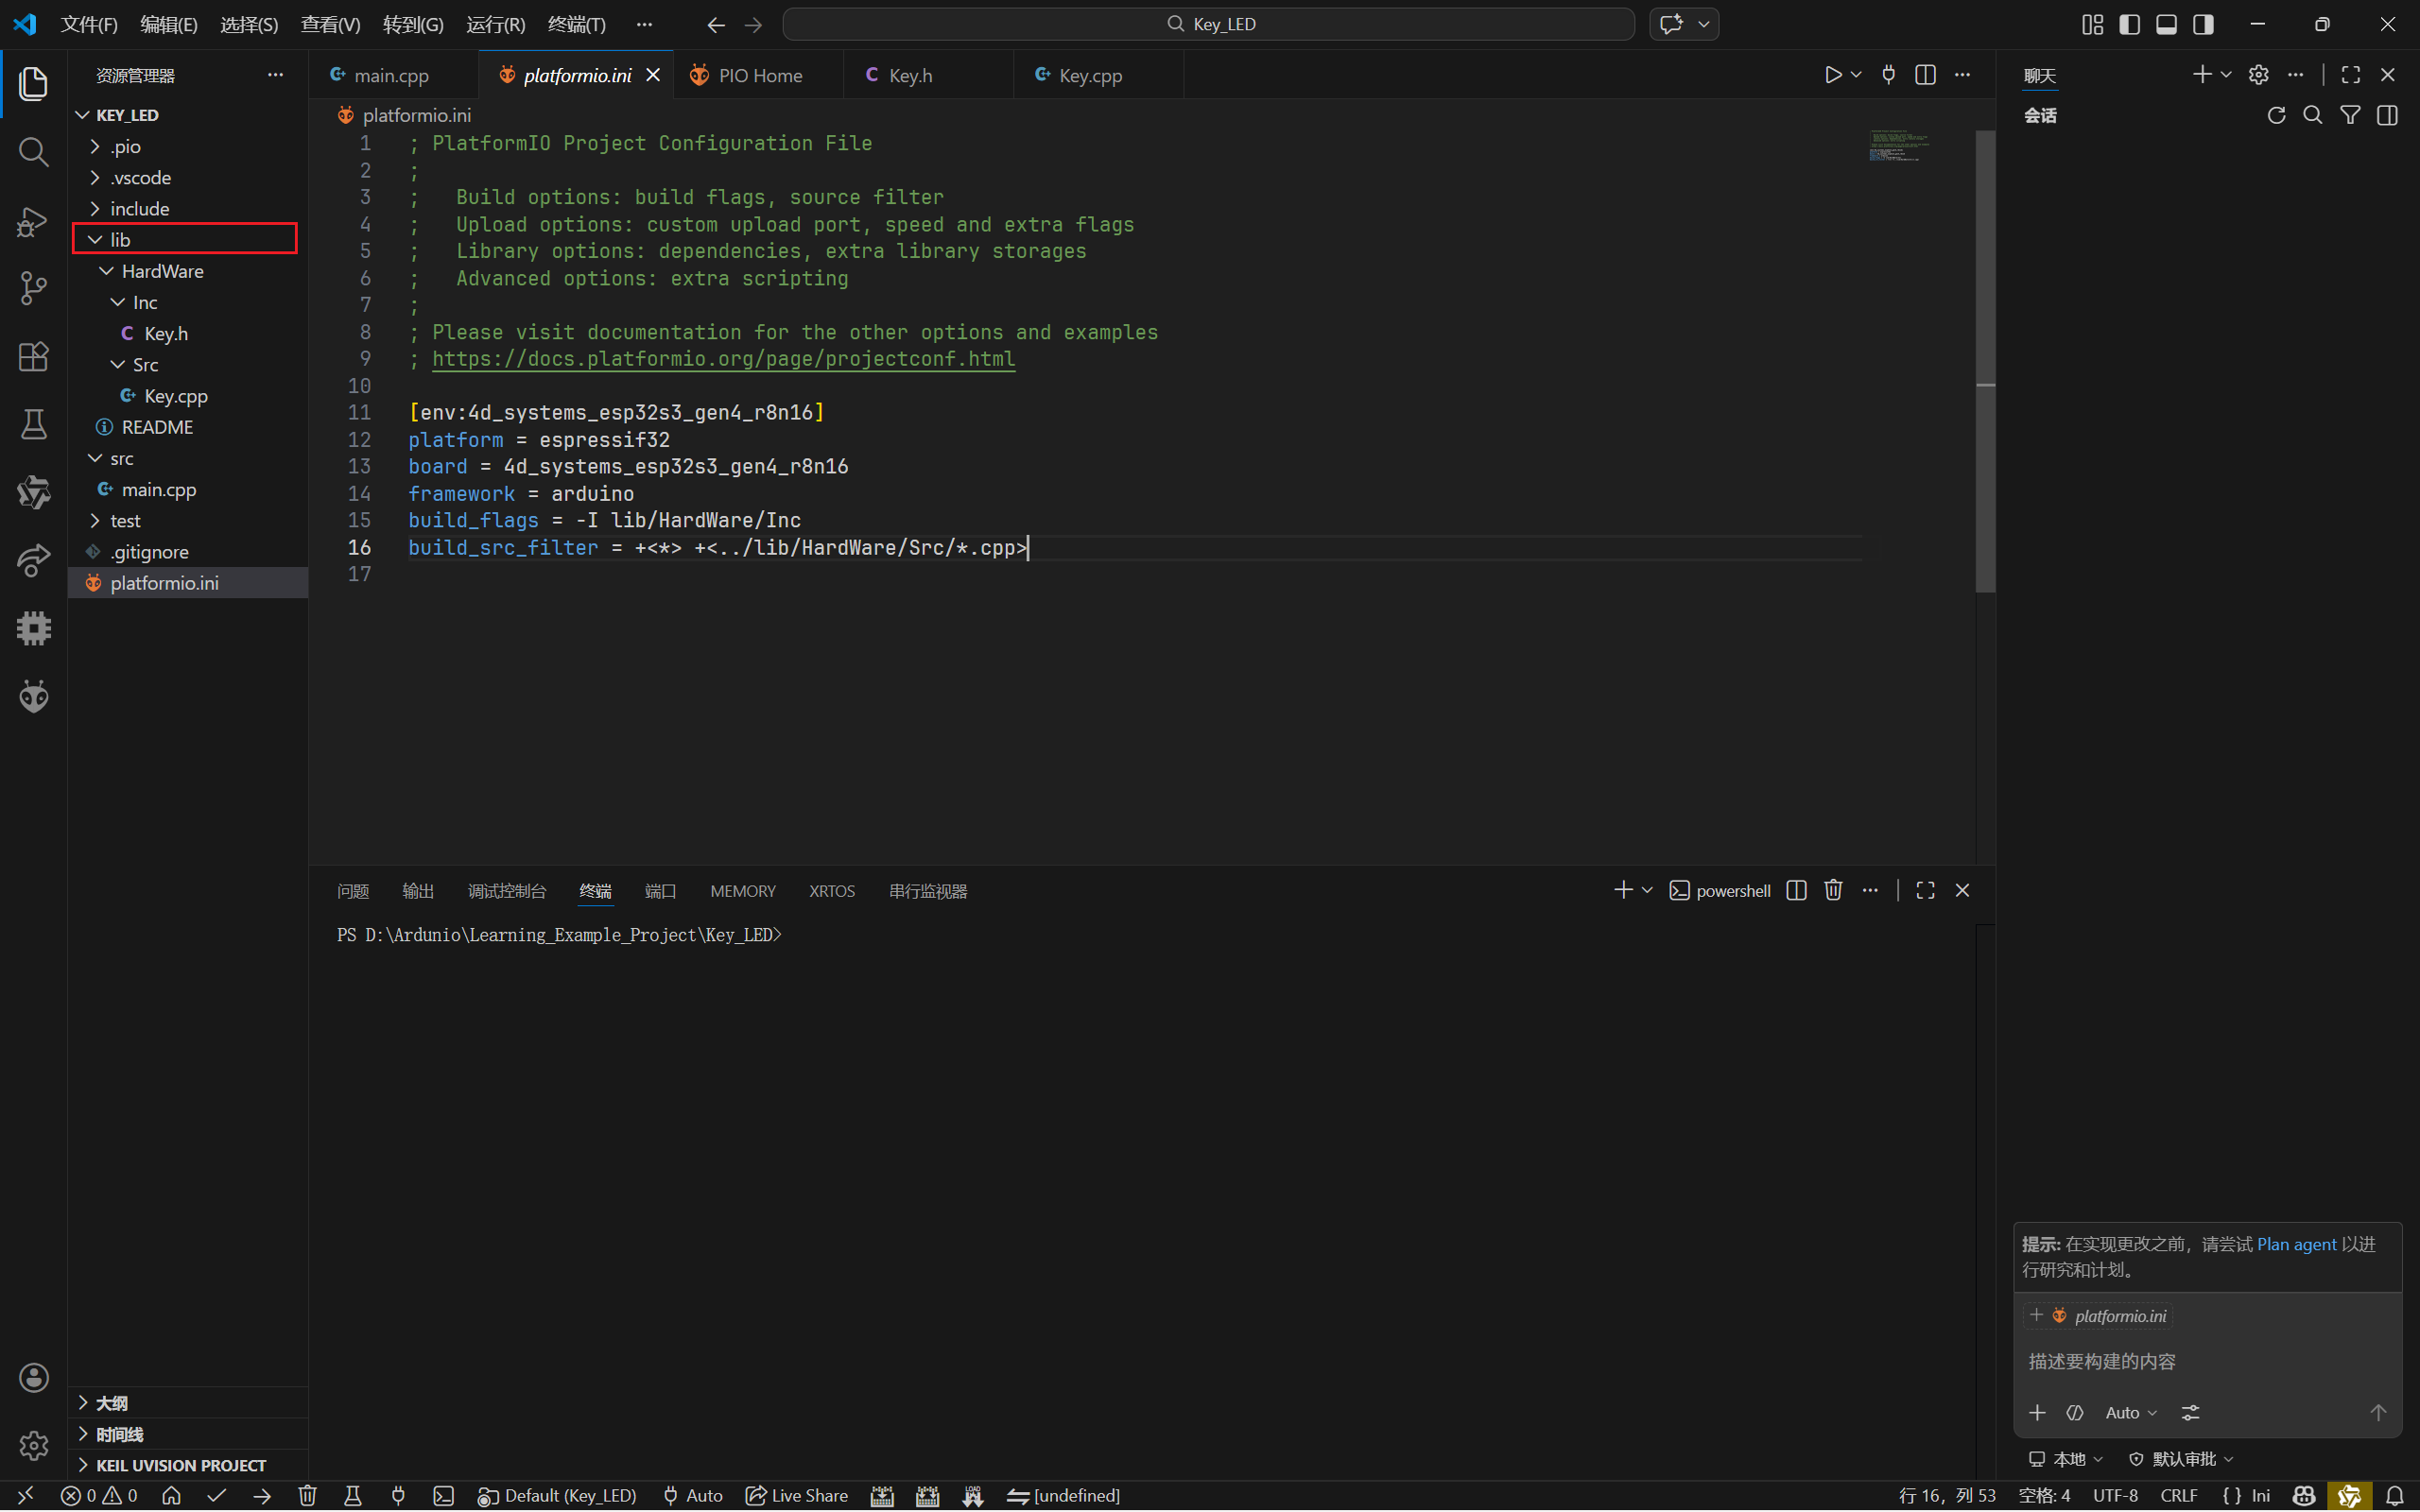
\includegraphics[width=\textwidth]{Figures/Document_Configue.png}
    \caption{多文件路径配置-1}
    
\end{figure}
\newpage
\indent 第二步, 在你所创立的文件夹下再建立 Inc 和 Src 文件夹, 分别用于存放.h 和.c 文件. 如图所示
\begin{figure}[h]
    \centering
    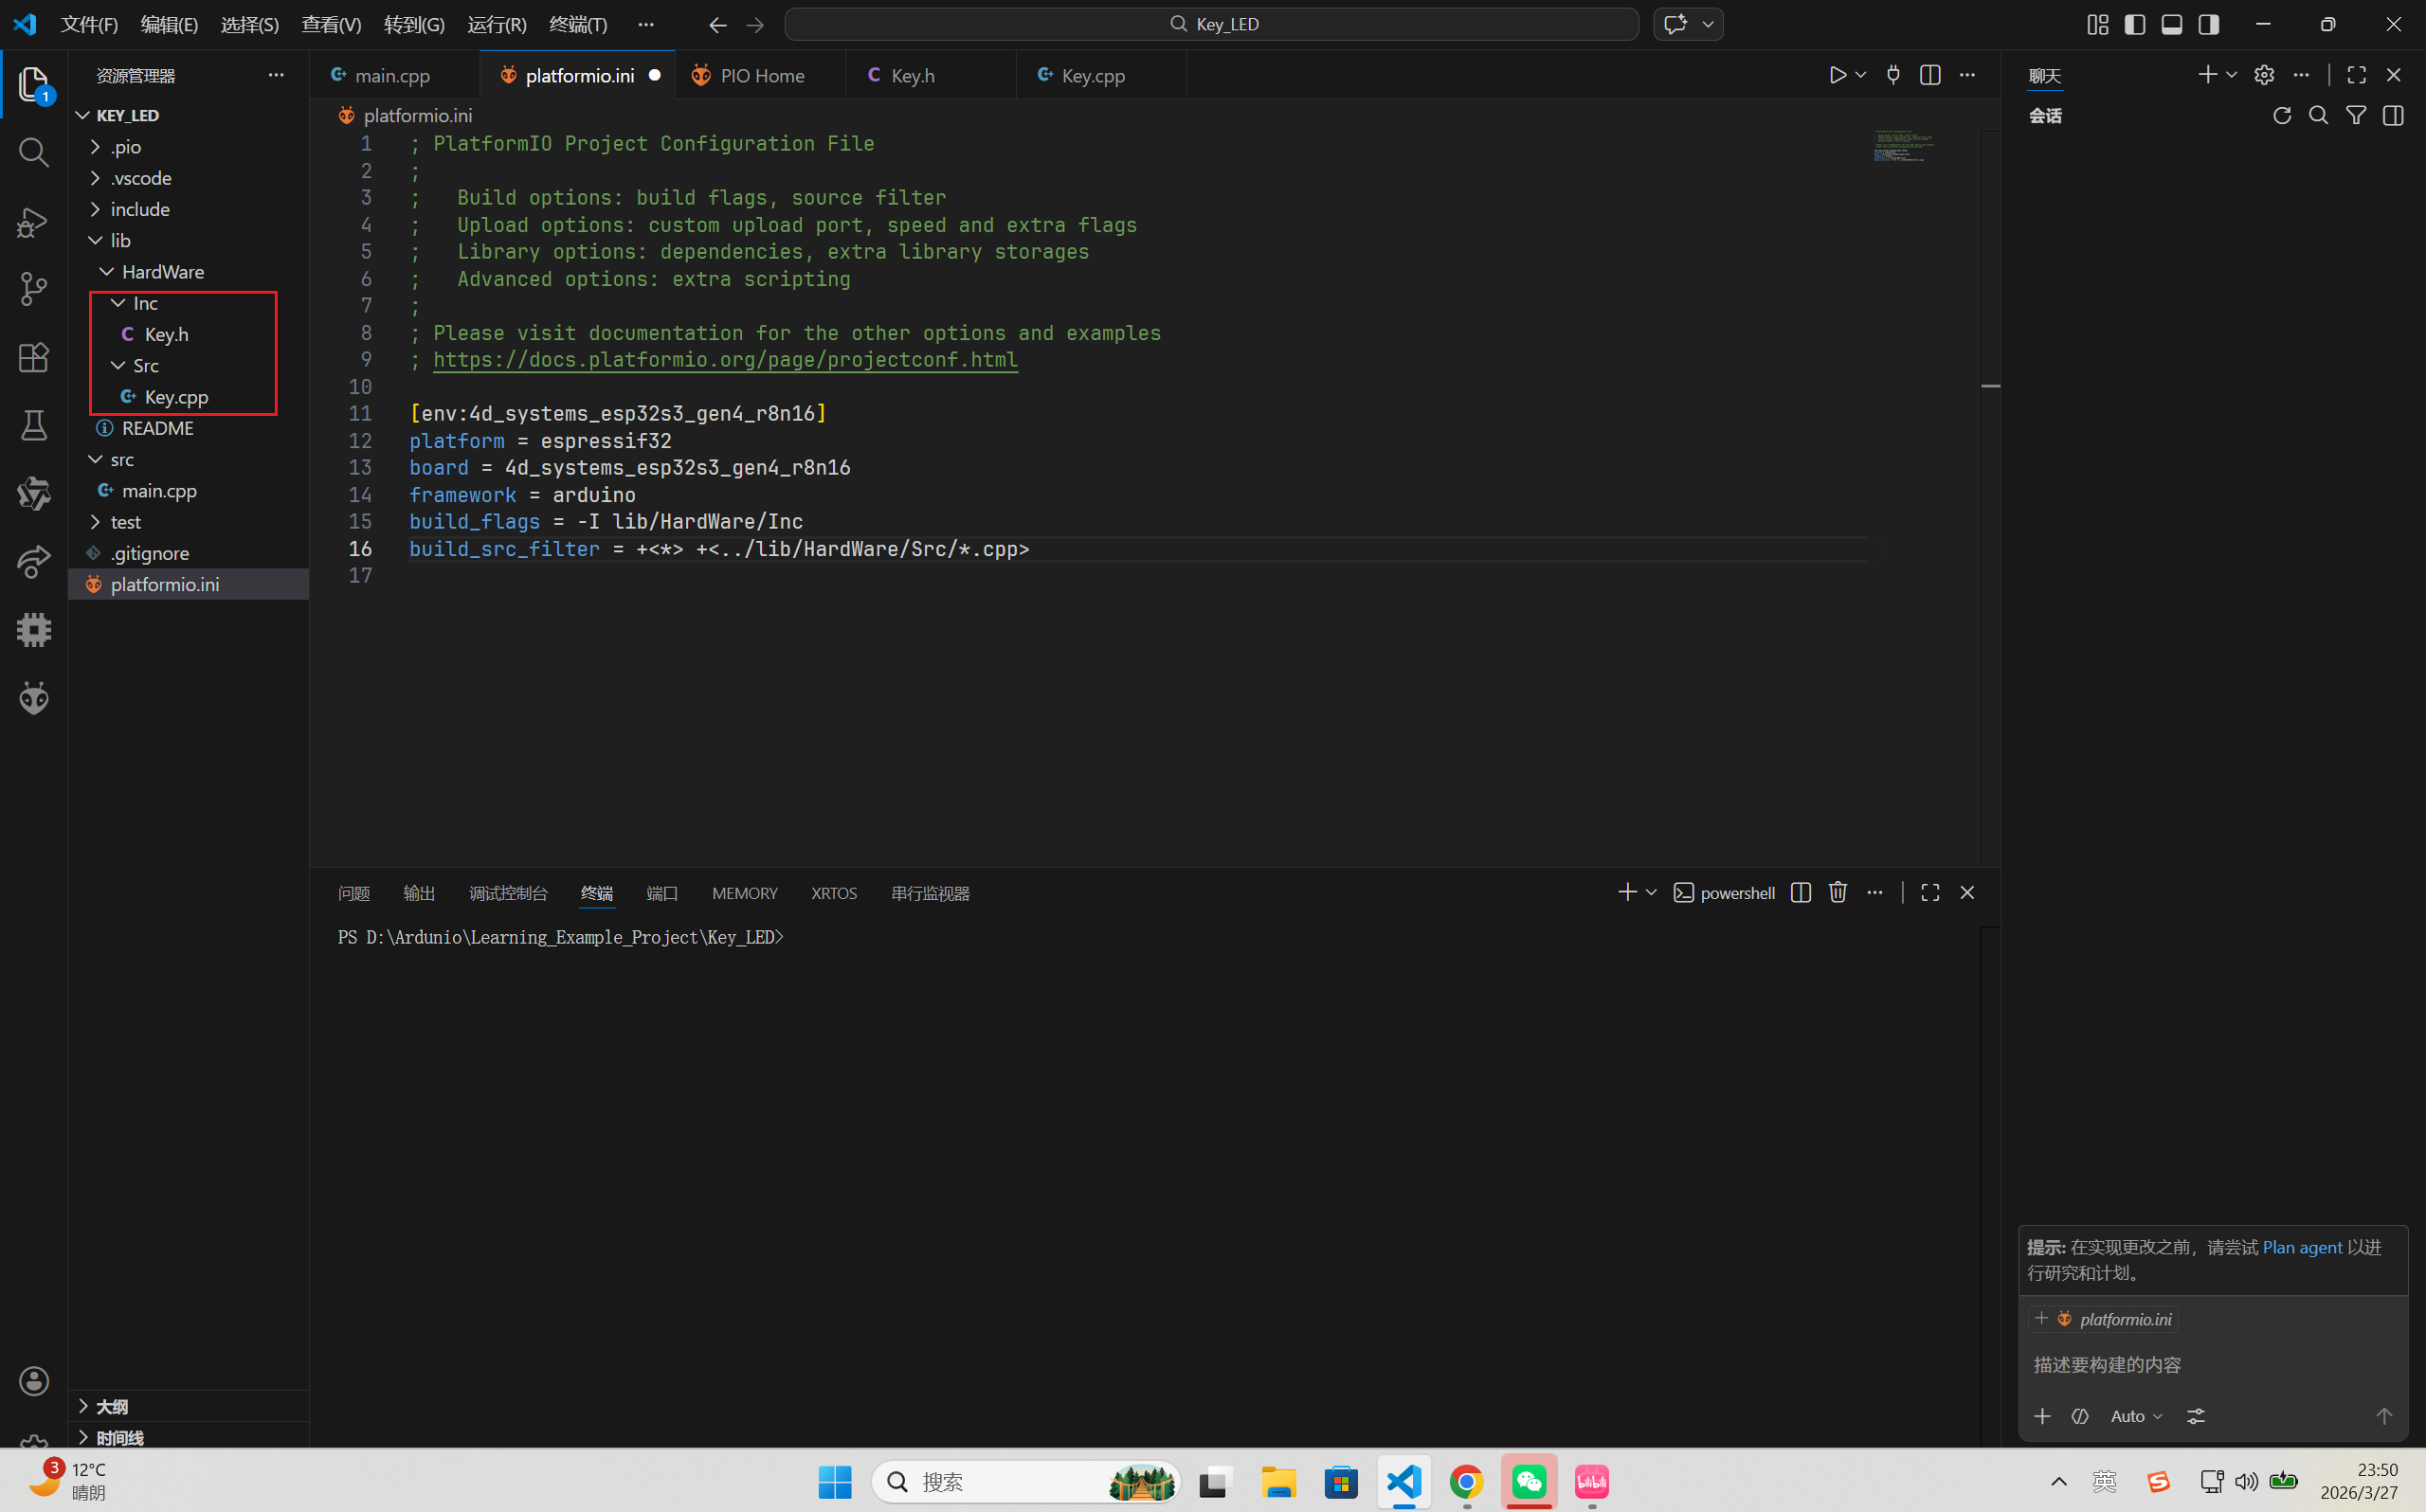
\includegraphics[width=\textwidth]{Figures/Second.png}
    \caption{多文件路径配置-2}

\end{figure}
\newpage
最后，在你的 \texttt{platformio.ini} 文件中添加这两行代码：
\texttt{build\_flags = -I lib/文件夹名/Inc} 和 
\texttt{build\_src\_filter = +<*> +<../lib/文件夹名/Src/*.cpp>} 
这两行代码表示让编译器在编译文件时，把这两个也加进去。
需要注意的是，我们新建文件是需要建立.cpp文件，如果只是.c文件的话，可能会出现各种奇奇怪怪的问题

\begin{figure}[h]
    \centering
    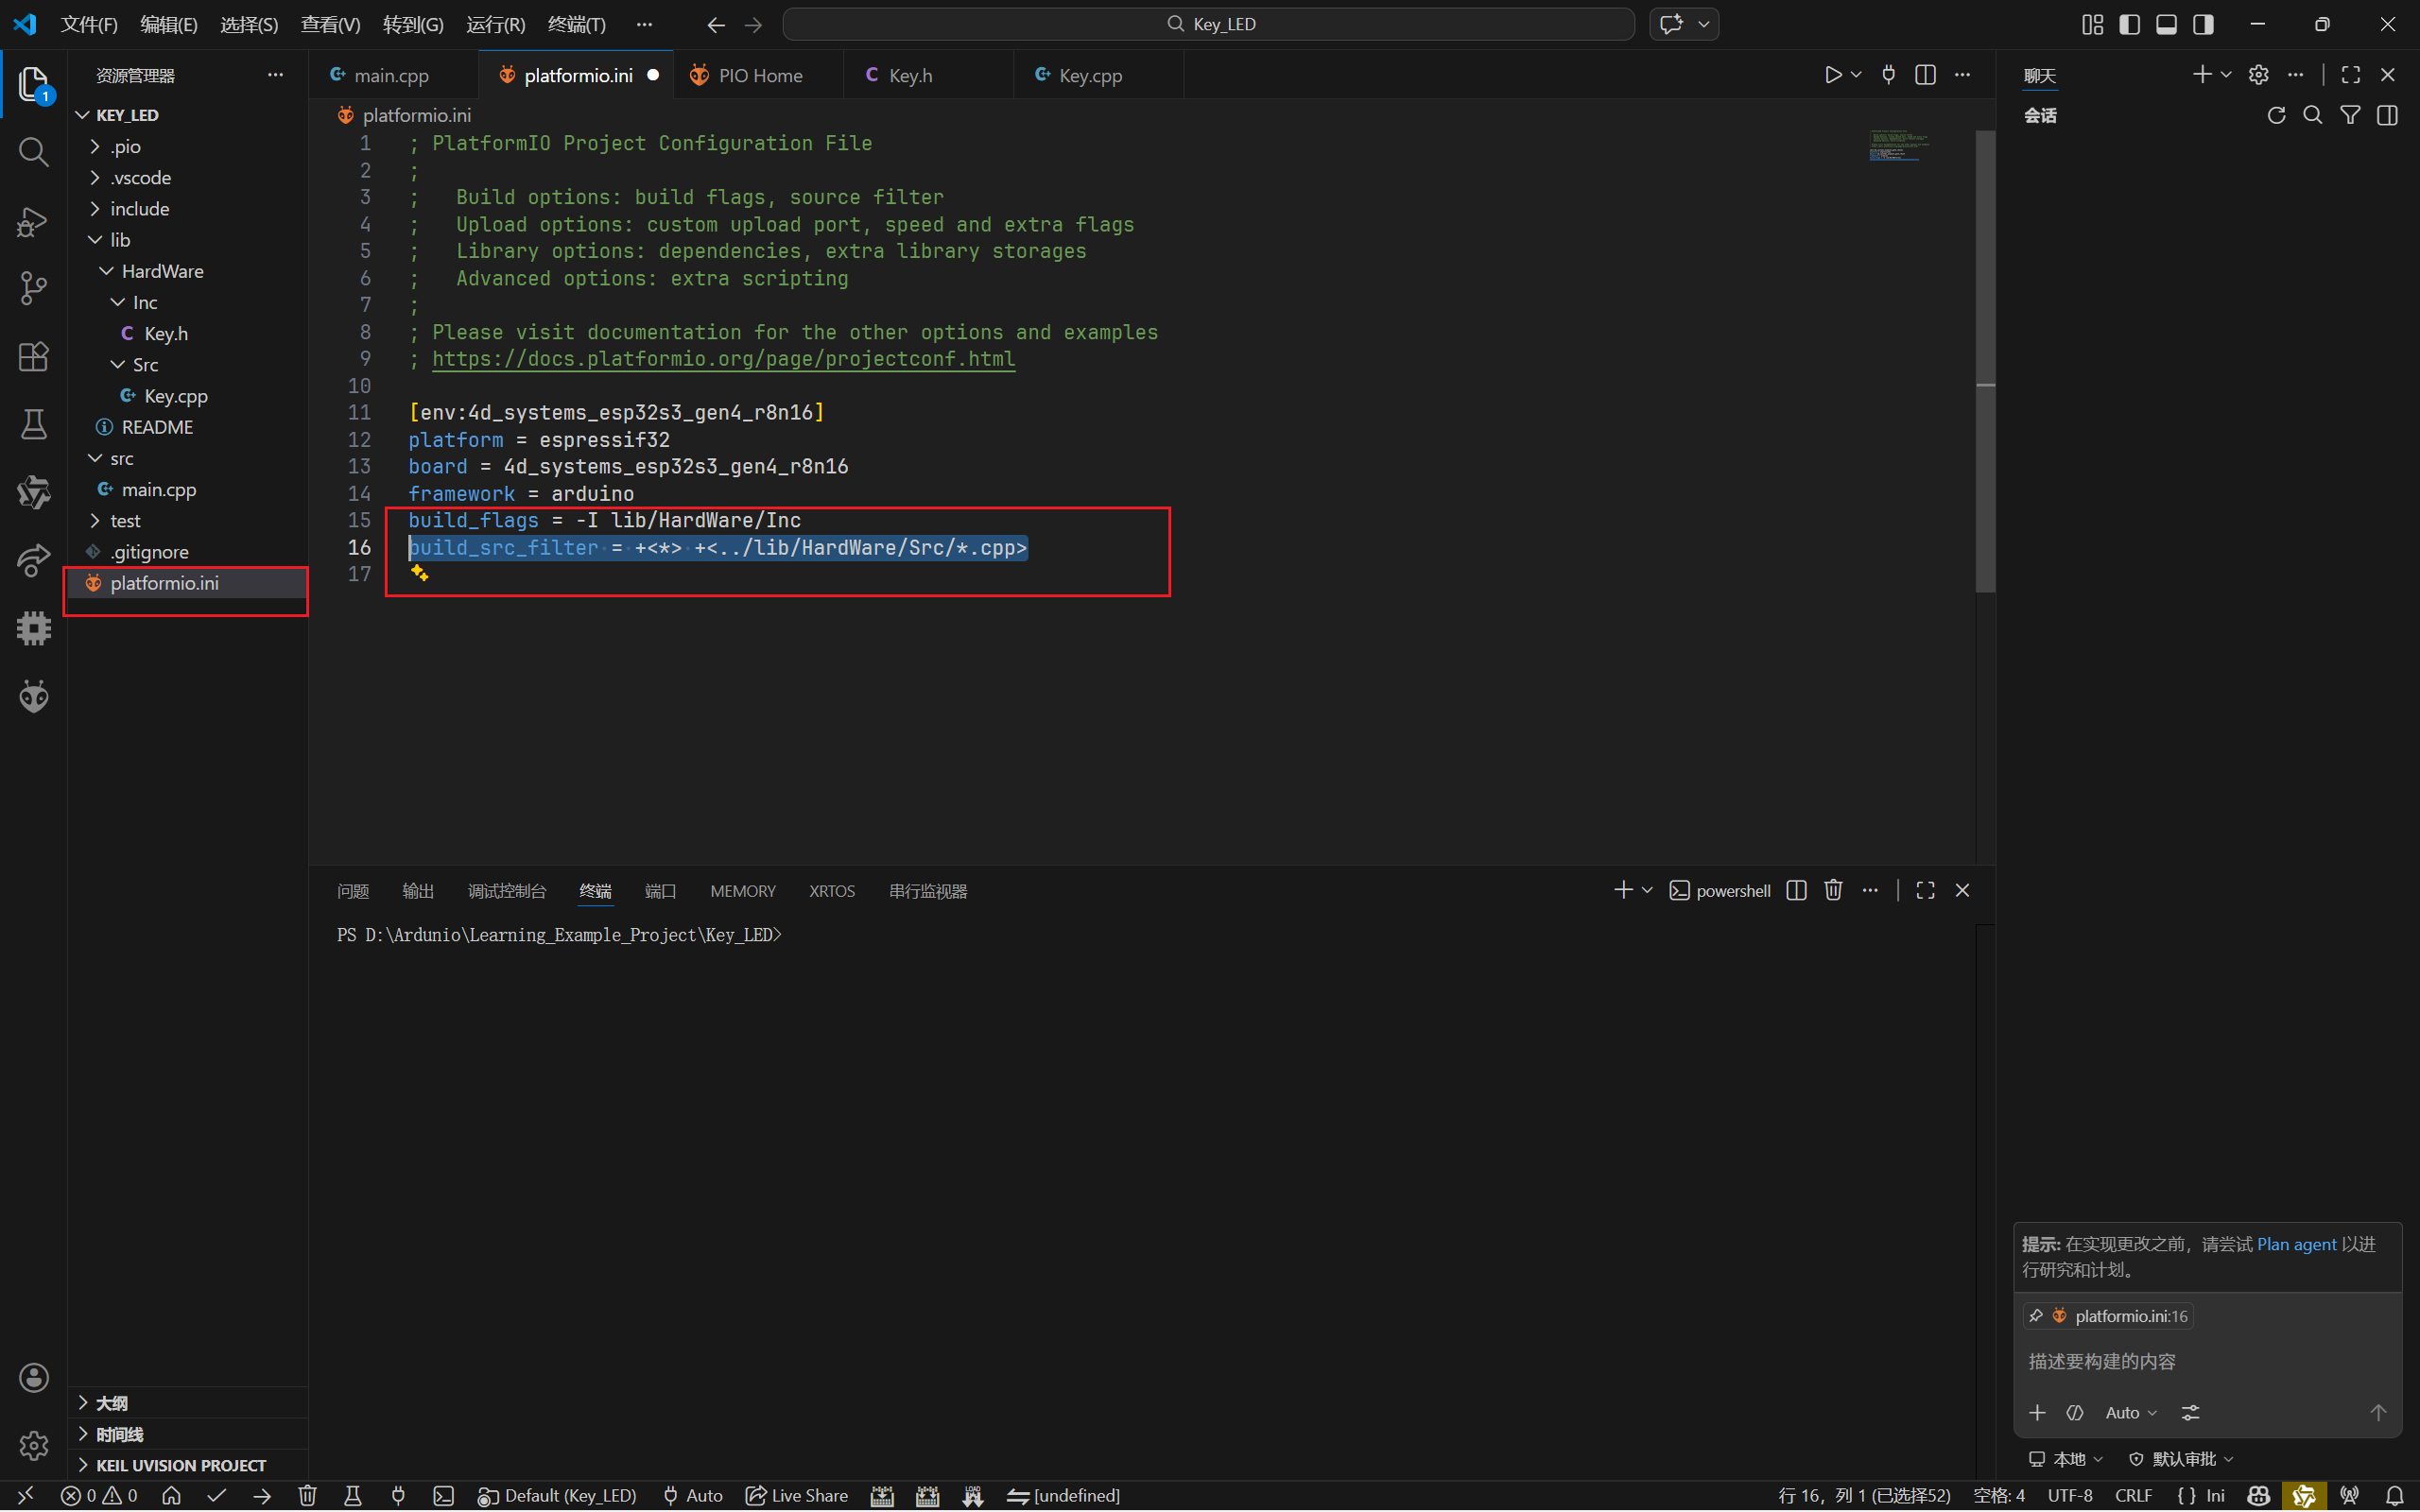
\includegraphics[width=\textwidth]{Figures/Third.png}
    \caption{多文件路径配置-3}
\end{figure}


% --- 内容结束 ---
\section{ 处理GPIO的相关函数 }
\subsection{ GPIO初始化函数,用于配置GPIO模式和引脚 }
\begin{figure}[h]
    \centering
    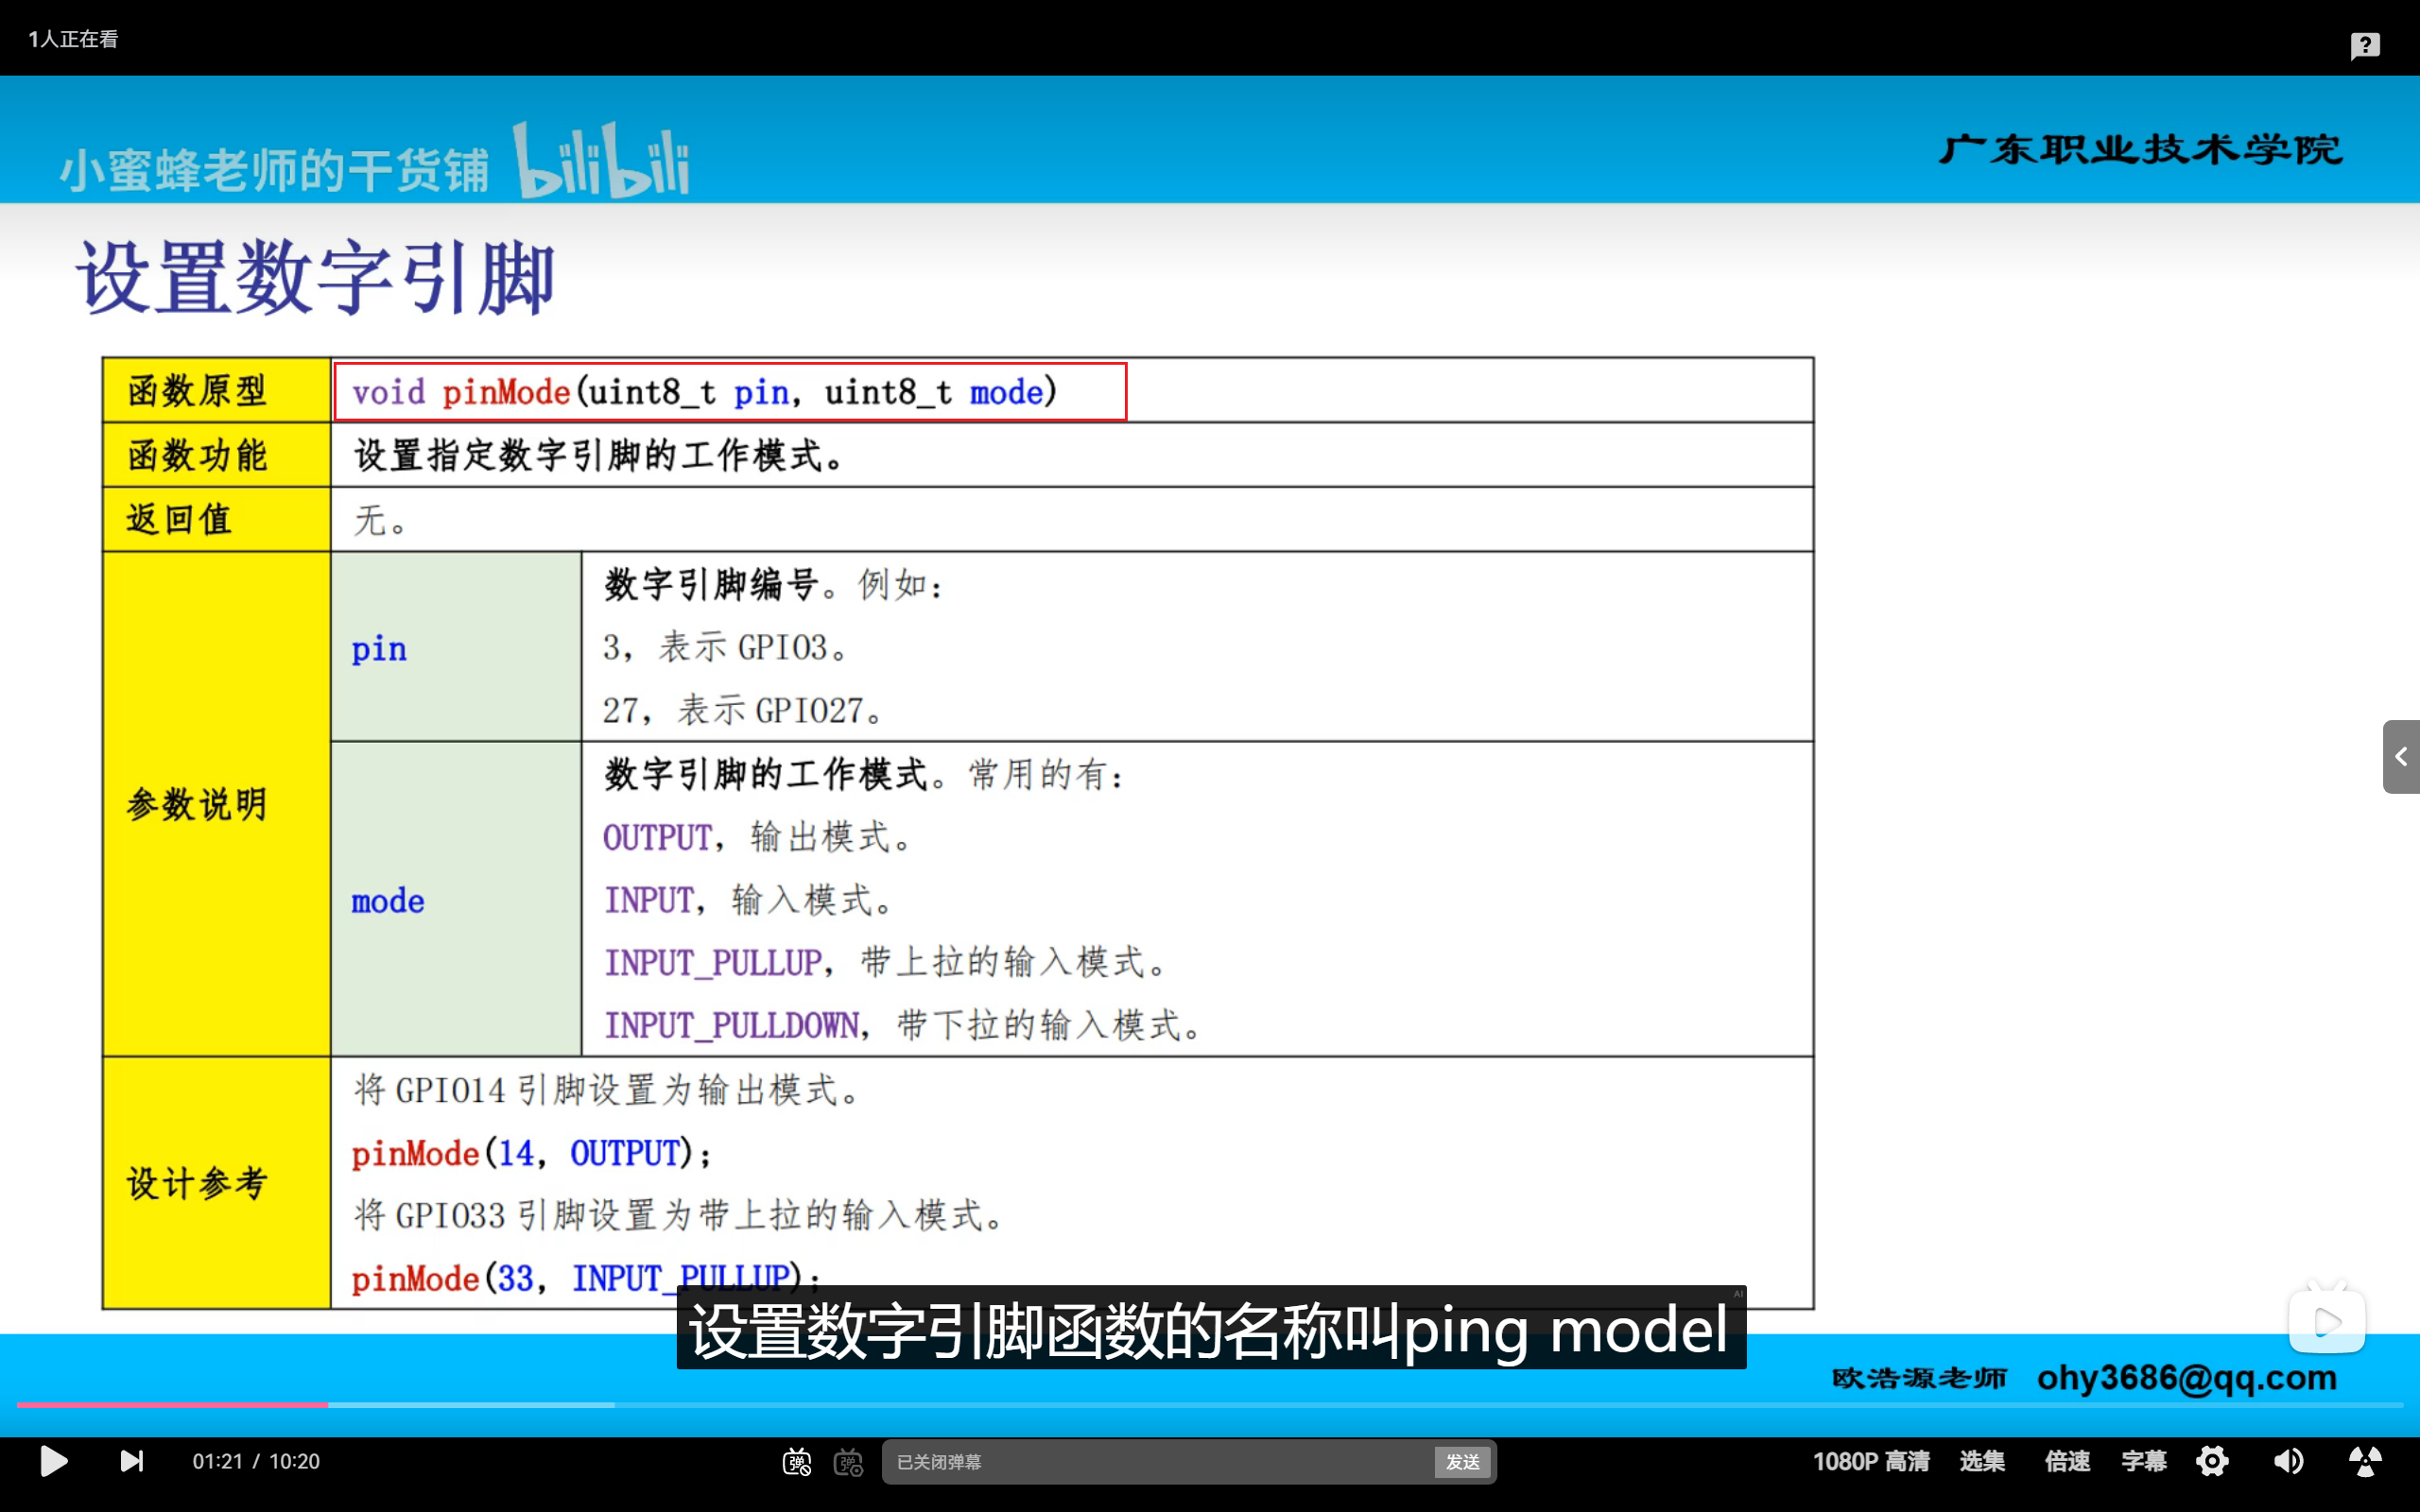
\includegraphics[width=\textwidth]{Figures/pinMode.png}
    \caption{pinMode}
    \label{fig:placeholder}
\end{figure}



函数名为: \textit{\textbf{void pinMode(参数一, 参数二)}}, 第一个参数为要初始化的引脚, 第二个参数为要设置的模式 
\newpage
\subsection{ GPIO引脚电平写入函数, 用于控制GPIO口的高低电平 }
\begin{figure}[h]
    \centering
    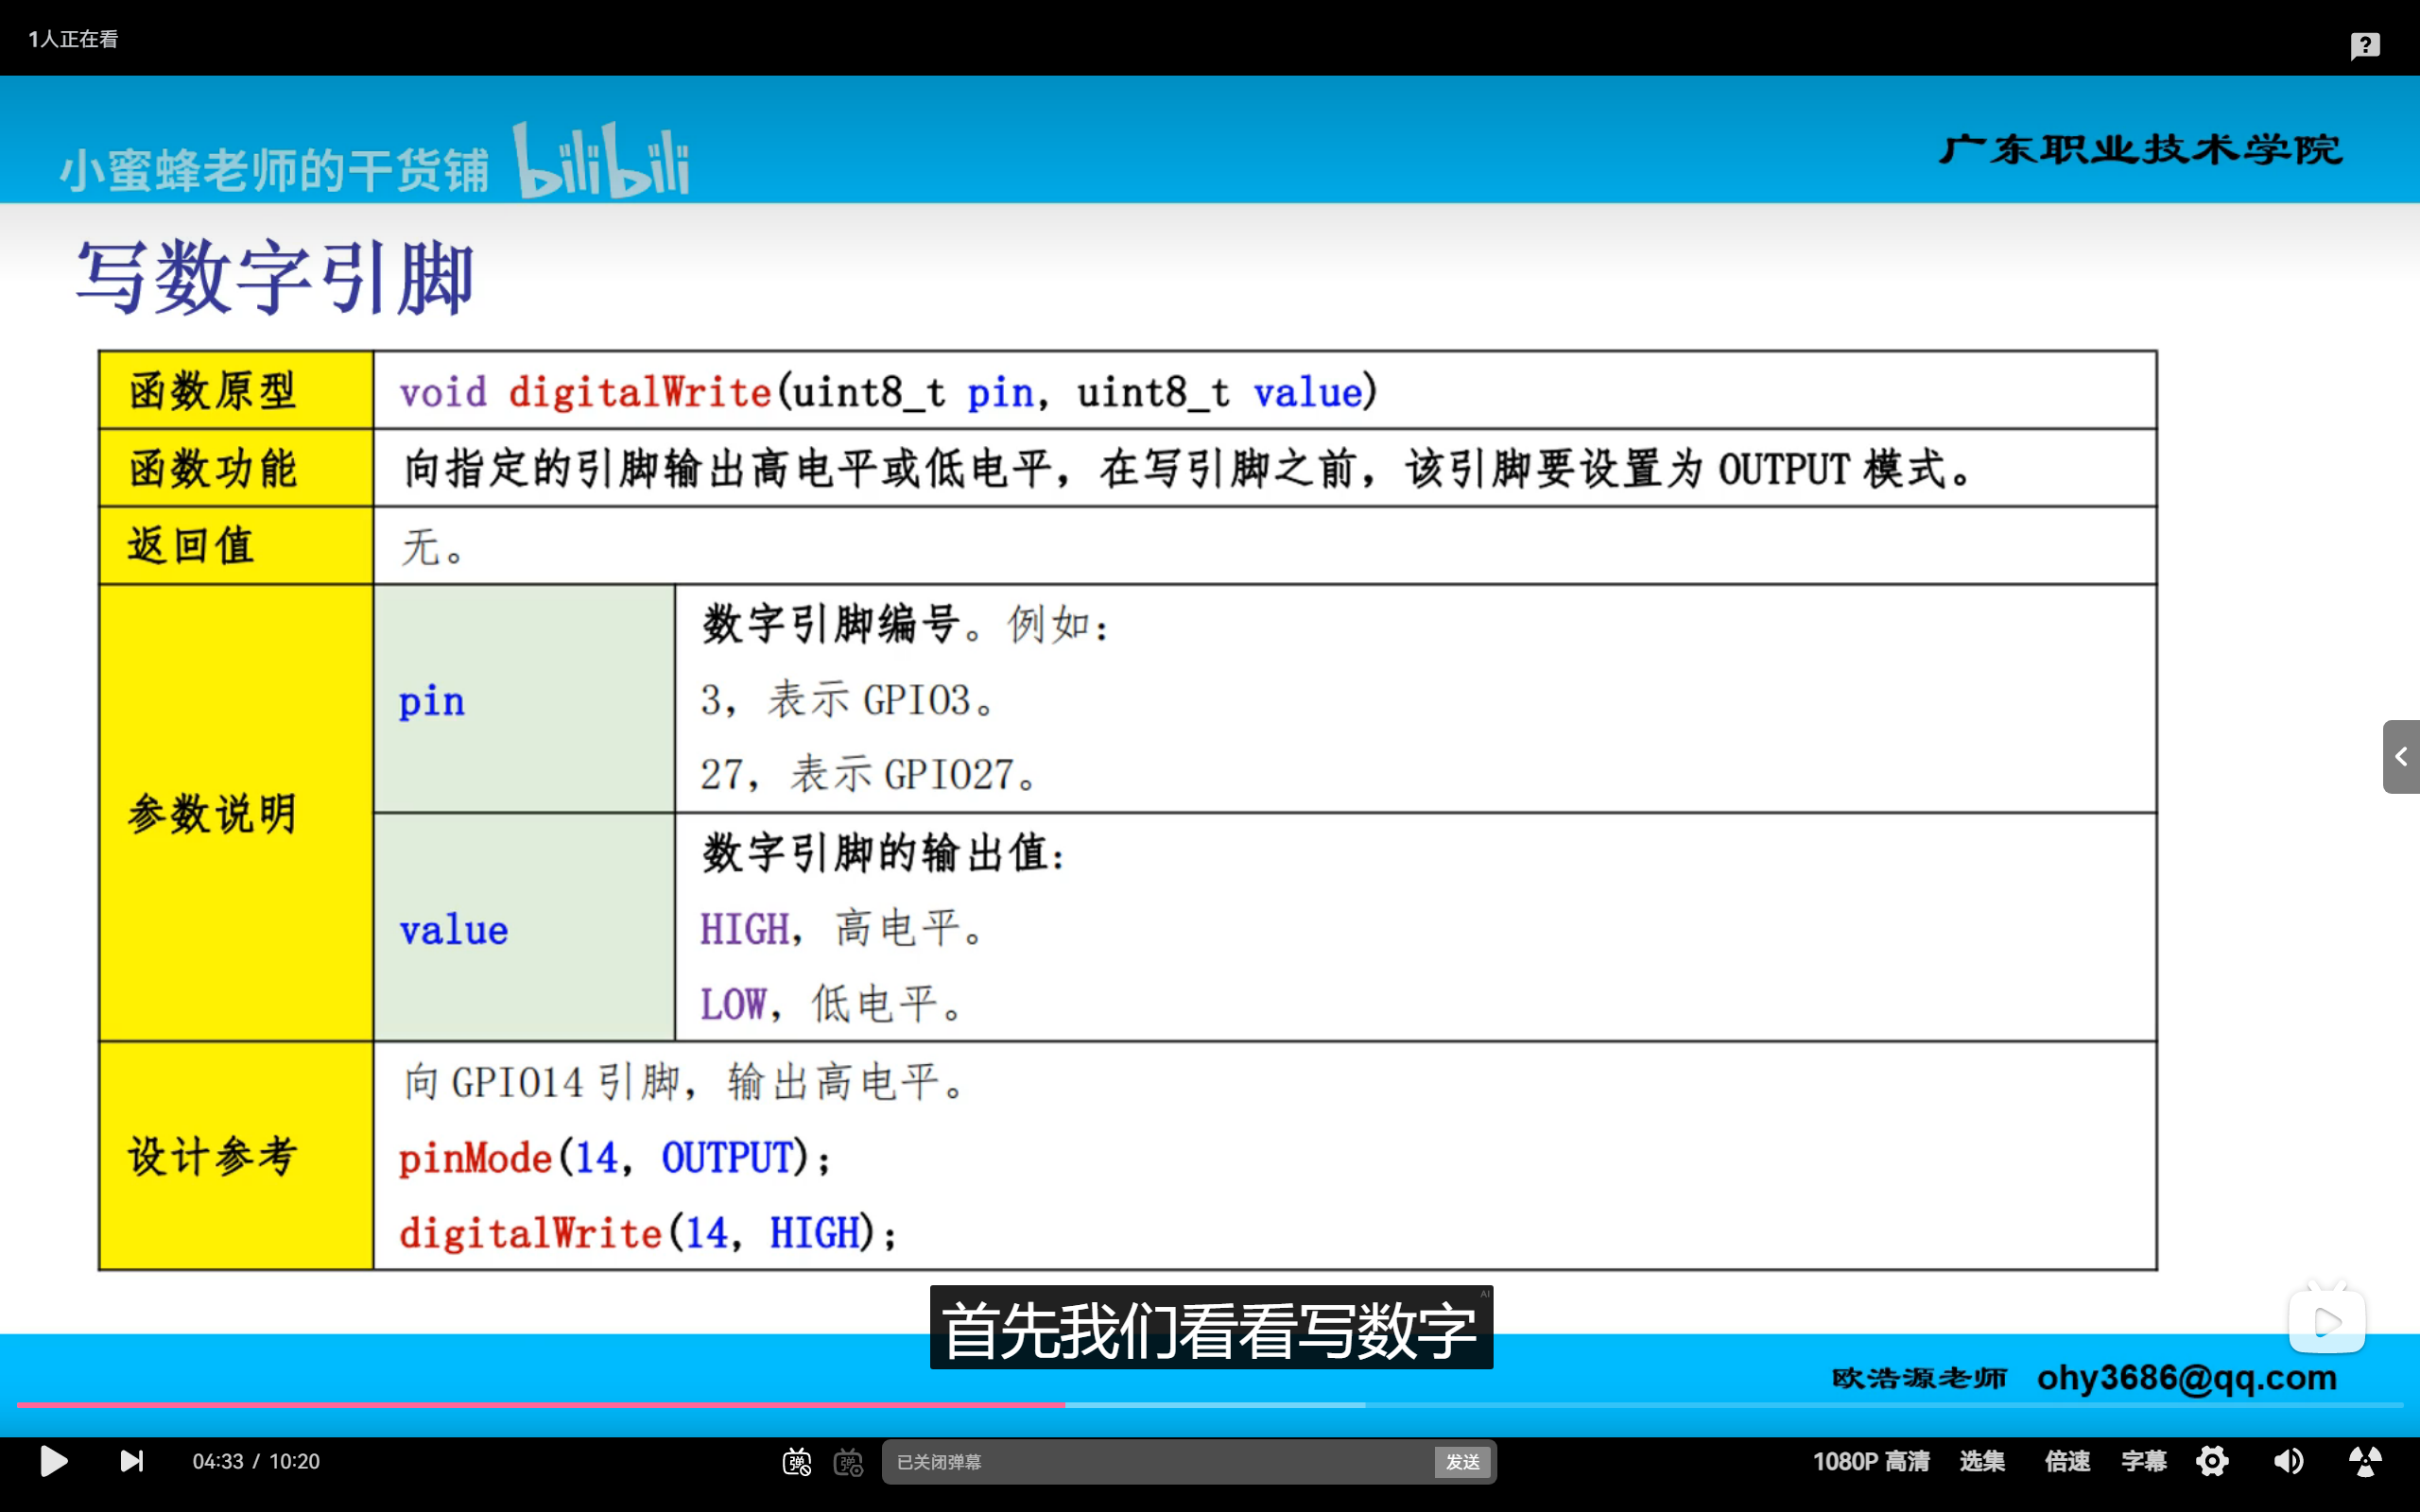
\includegraphics[width = \textwidth]{Figures/exemple.png}
    \caption{电平写入函数}
    
\end{figure}
函数名为: \textit{\textbf{digitalWrite(参数一,参数二)}}, 第一个参数表示引脚, 第二个参数表示Value(有HIGH和LOW)

\newpage
\subsection{ GPIO引脚电平读取函数, 用于获取GPIO口的高低电平 }
\begin{figure}[h]
    \centering
    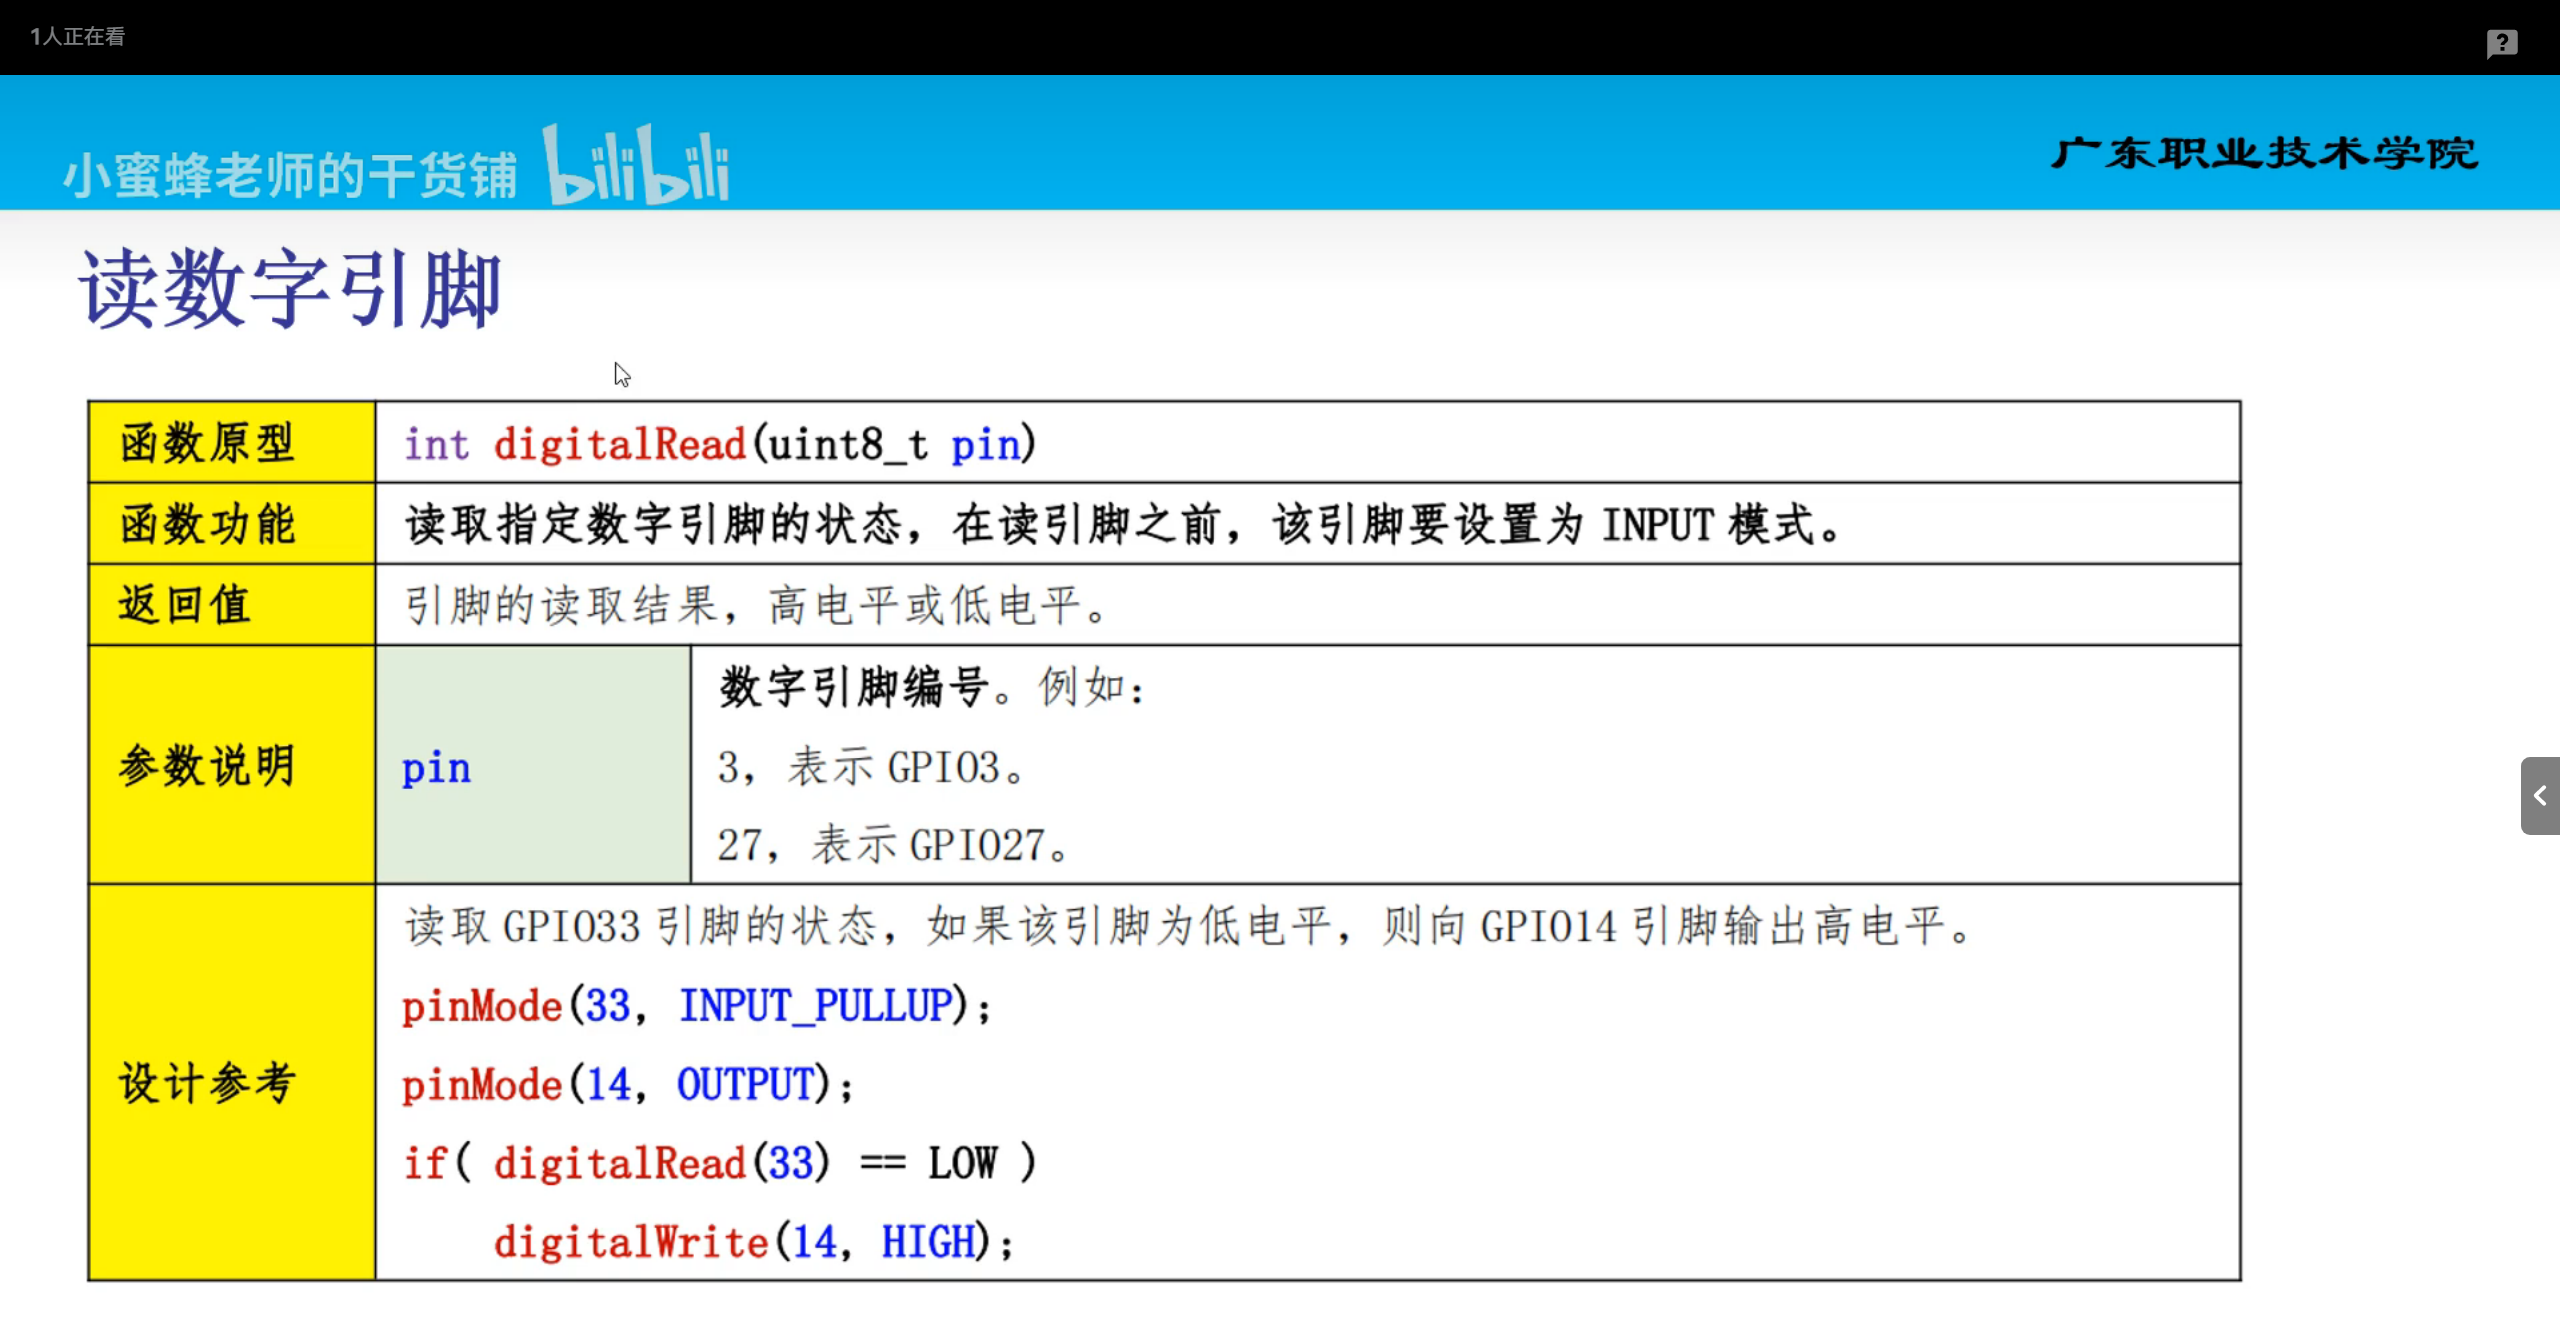
\includegraphics[width=\textwidth]{Figures/digitalRead.png}
    \caption{digitalRead}
   
\end{figure}
函数名为: \textit{\textbf{void digitalRead(参数一)}},参数一为要读取的引脚


\section{ 处理PWM的相关函数 }
\subsection{ PWM初始化函数, 用于初始化PWM配置 }
\begin{figure}[h]
    \centering
    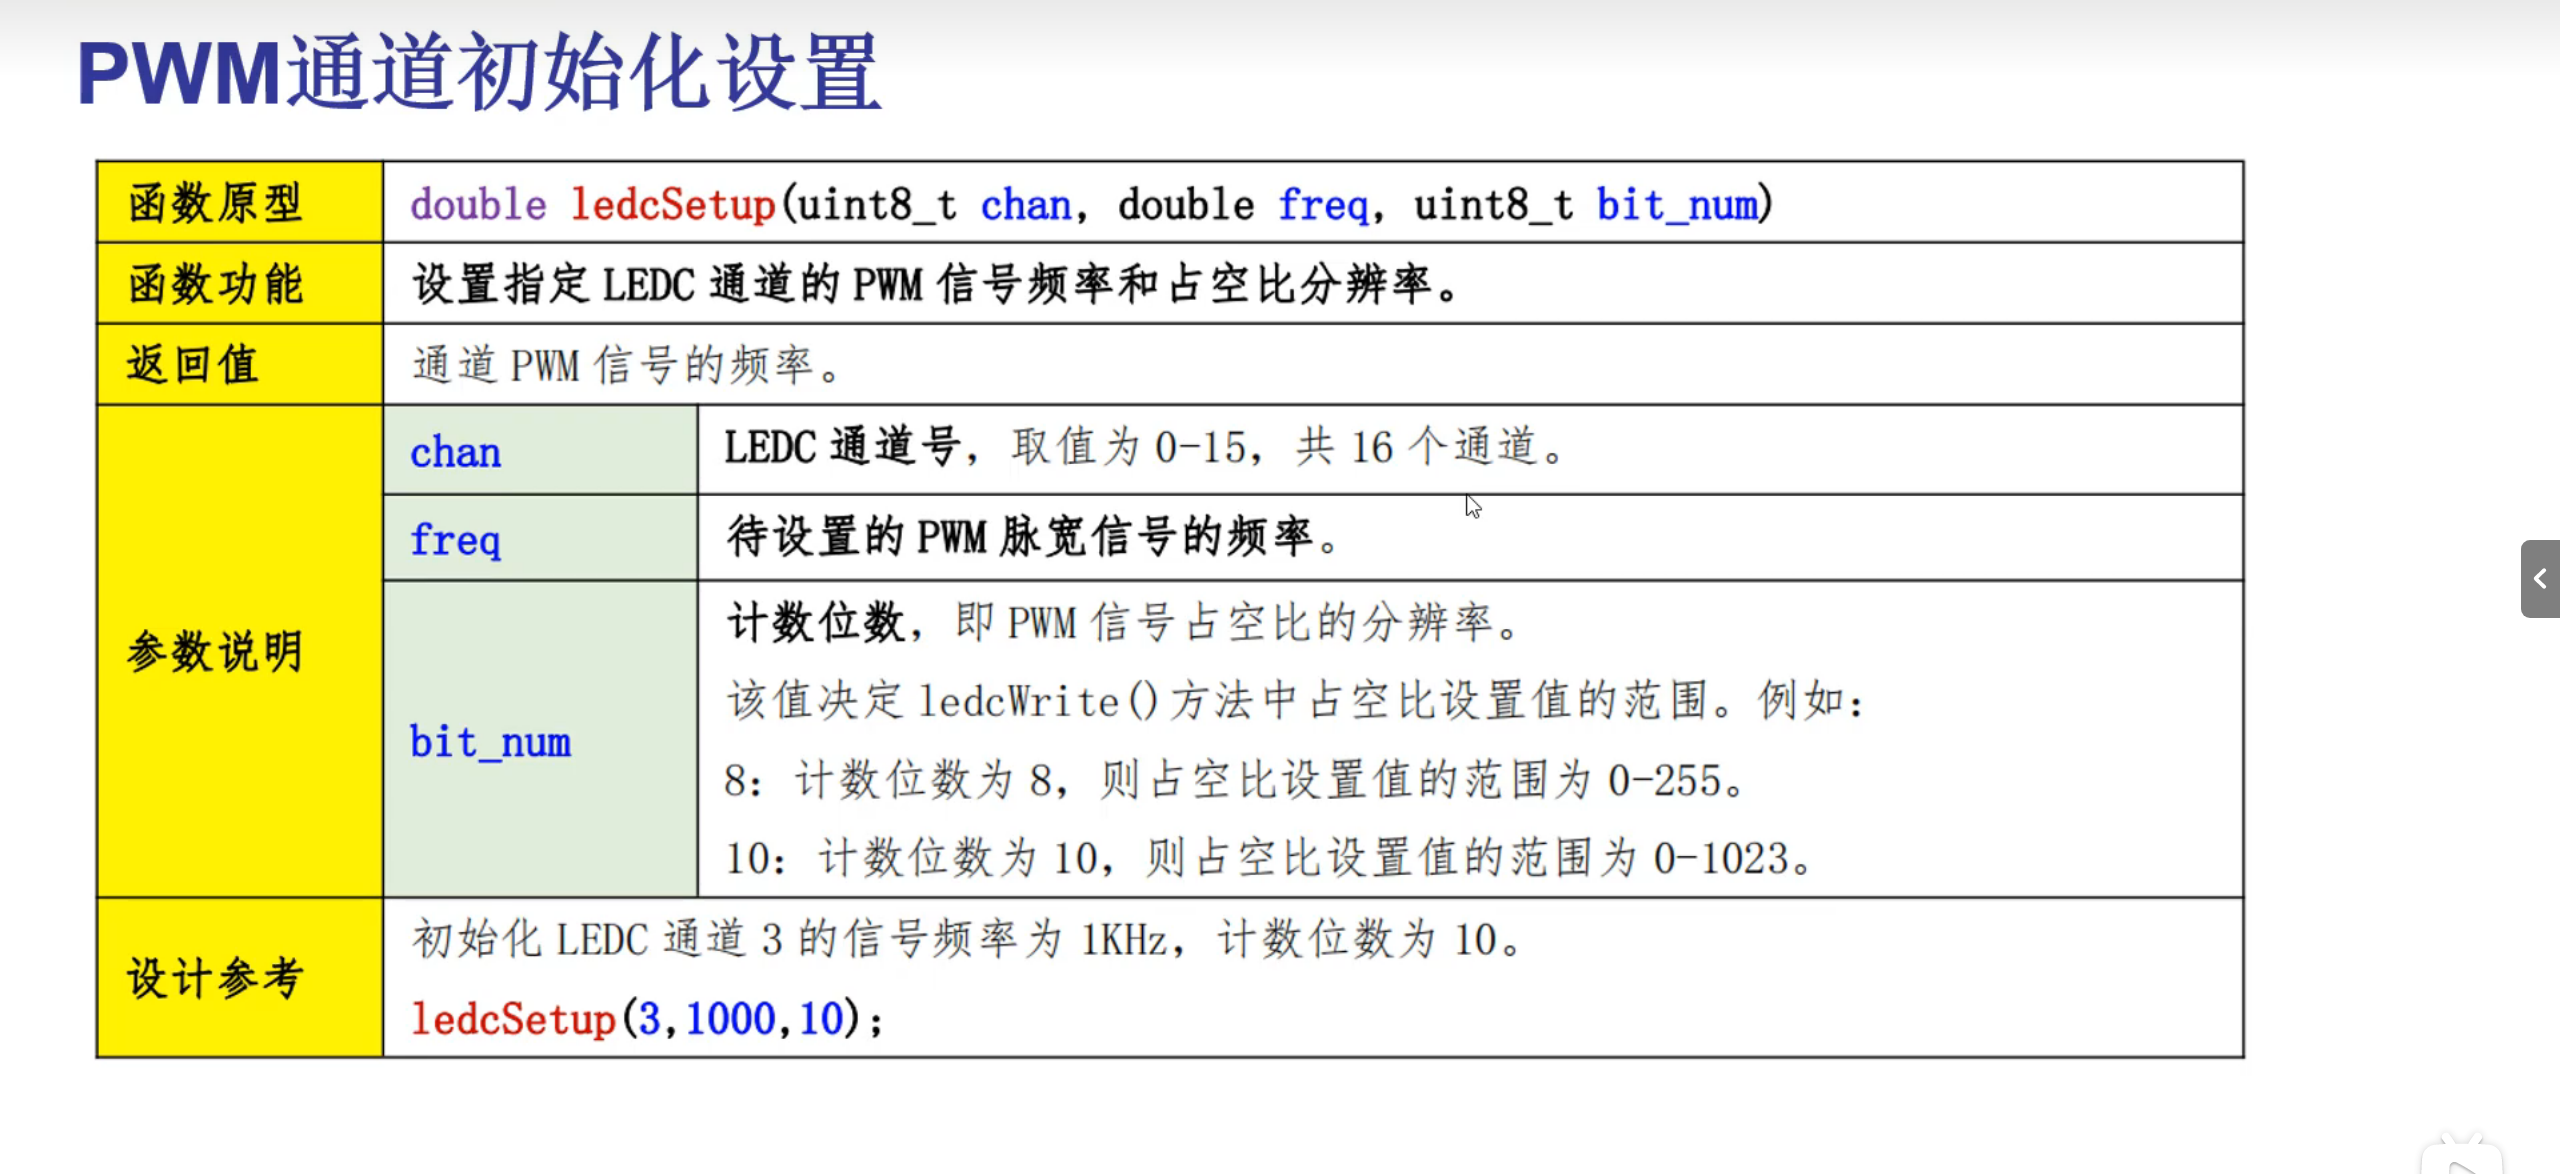
\includegraphics[width=0.6\textwidth]{Figures/ledcSetup.png}
    \caption{ledcSetup}
   
\end{figure}
函数名为:\textit{ \textbf{ void ledcSetup(参数一,参数二,参数三)}  },参数一为要绑定的通道;参数二为PWM频率;参数三为计数位数
\subsection{ PWM通道绑定函数, 用于使能某个特定的引脚输出PWM波 }
\begin{figure}[h]
    \centering
    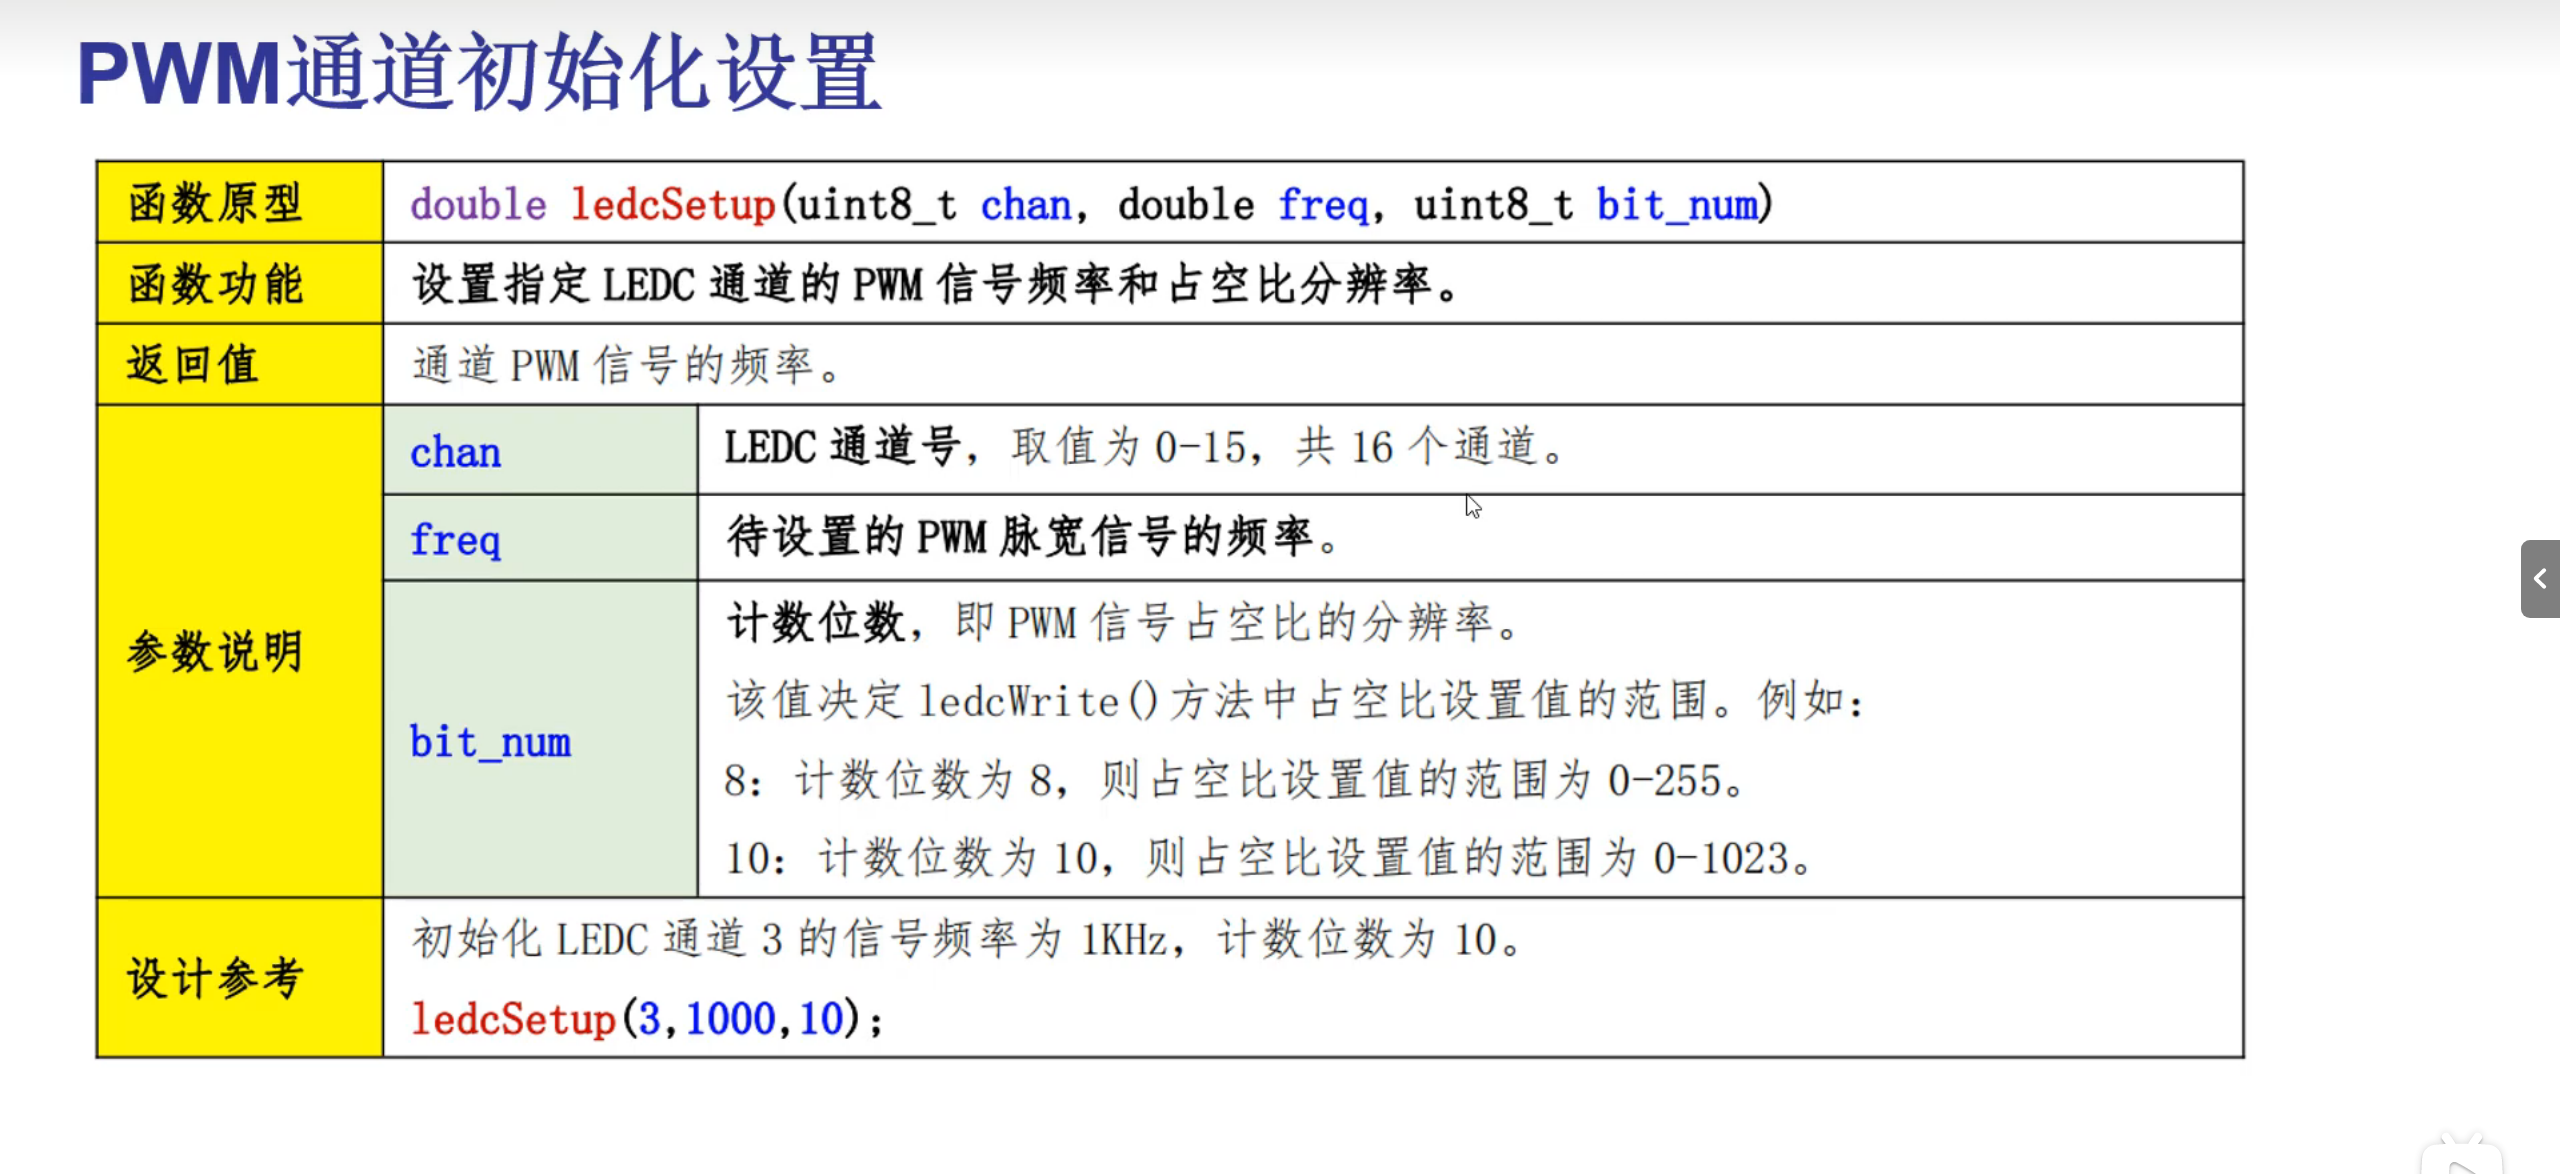
\includegraphics[width=\textwidth]{Figures/ledcAttachPin.png}
    \caption{ledaAttachPin}    
\end{figure}
函数名为:\textit{ \textbf{void ledcAttachPin(参数一,参数二)}}.参数一为要指定的引脚,参数二表示要用哪个通道输出的PWM波

\subsection{ PWM占空比设置函数 }
函数名为: \textit{ \textbf{void ledcWrite(参数一, 参数二 )} }.参数一为要进行操作的PWM通道;参数二为占空比数值
\begin{figure}[h]
    \centering
    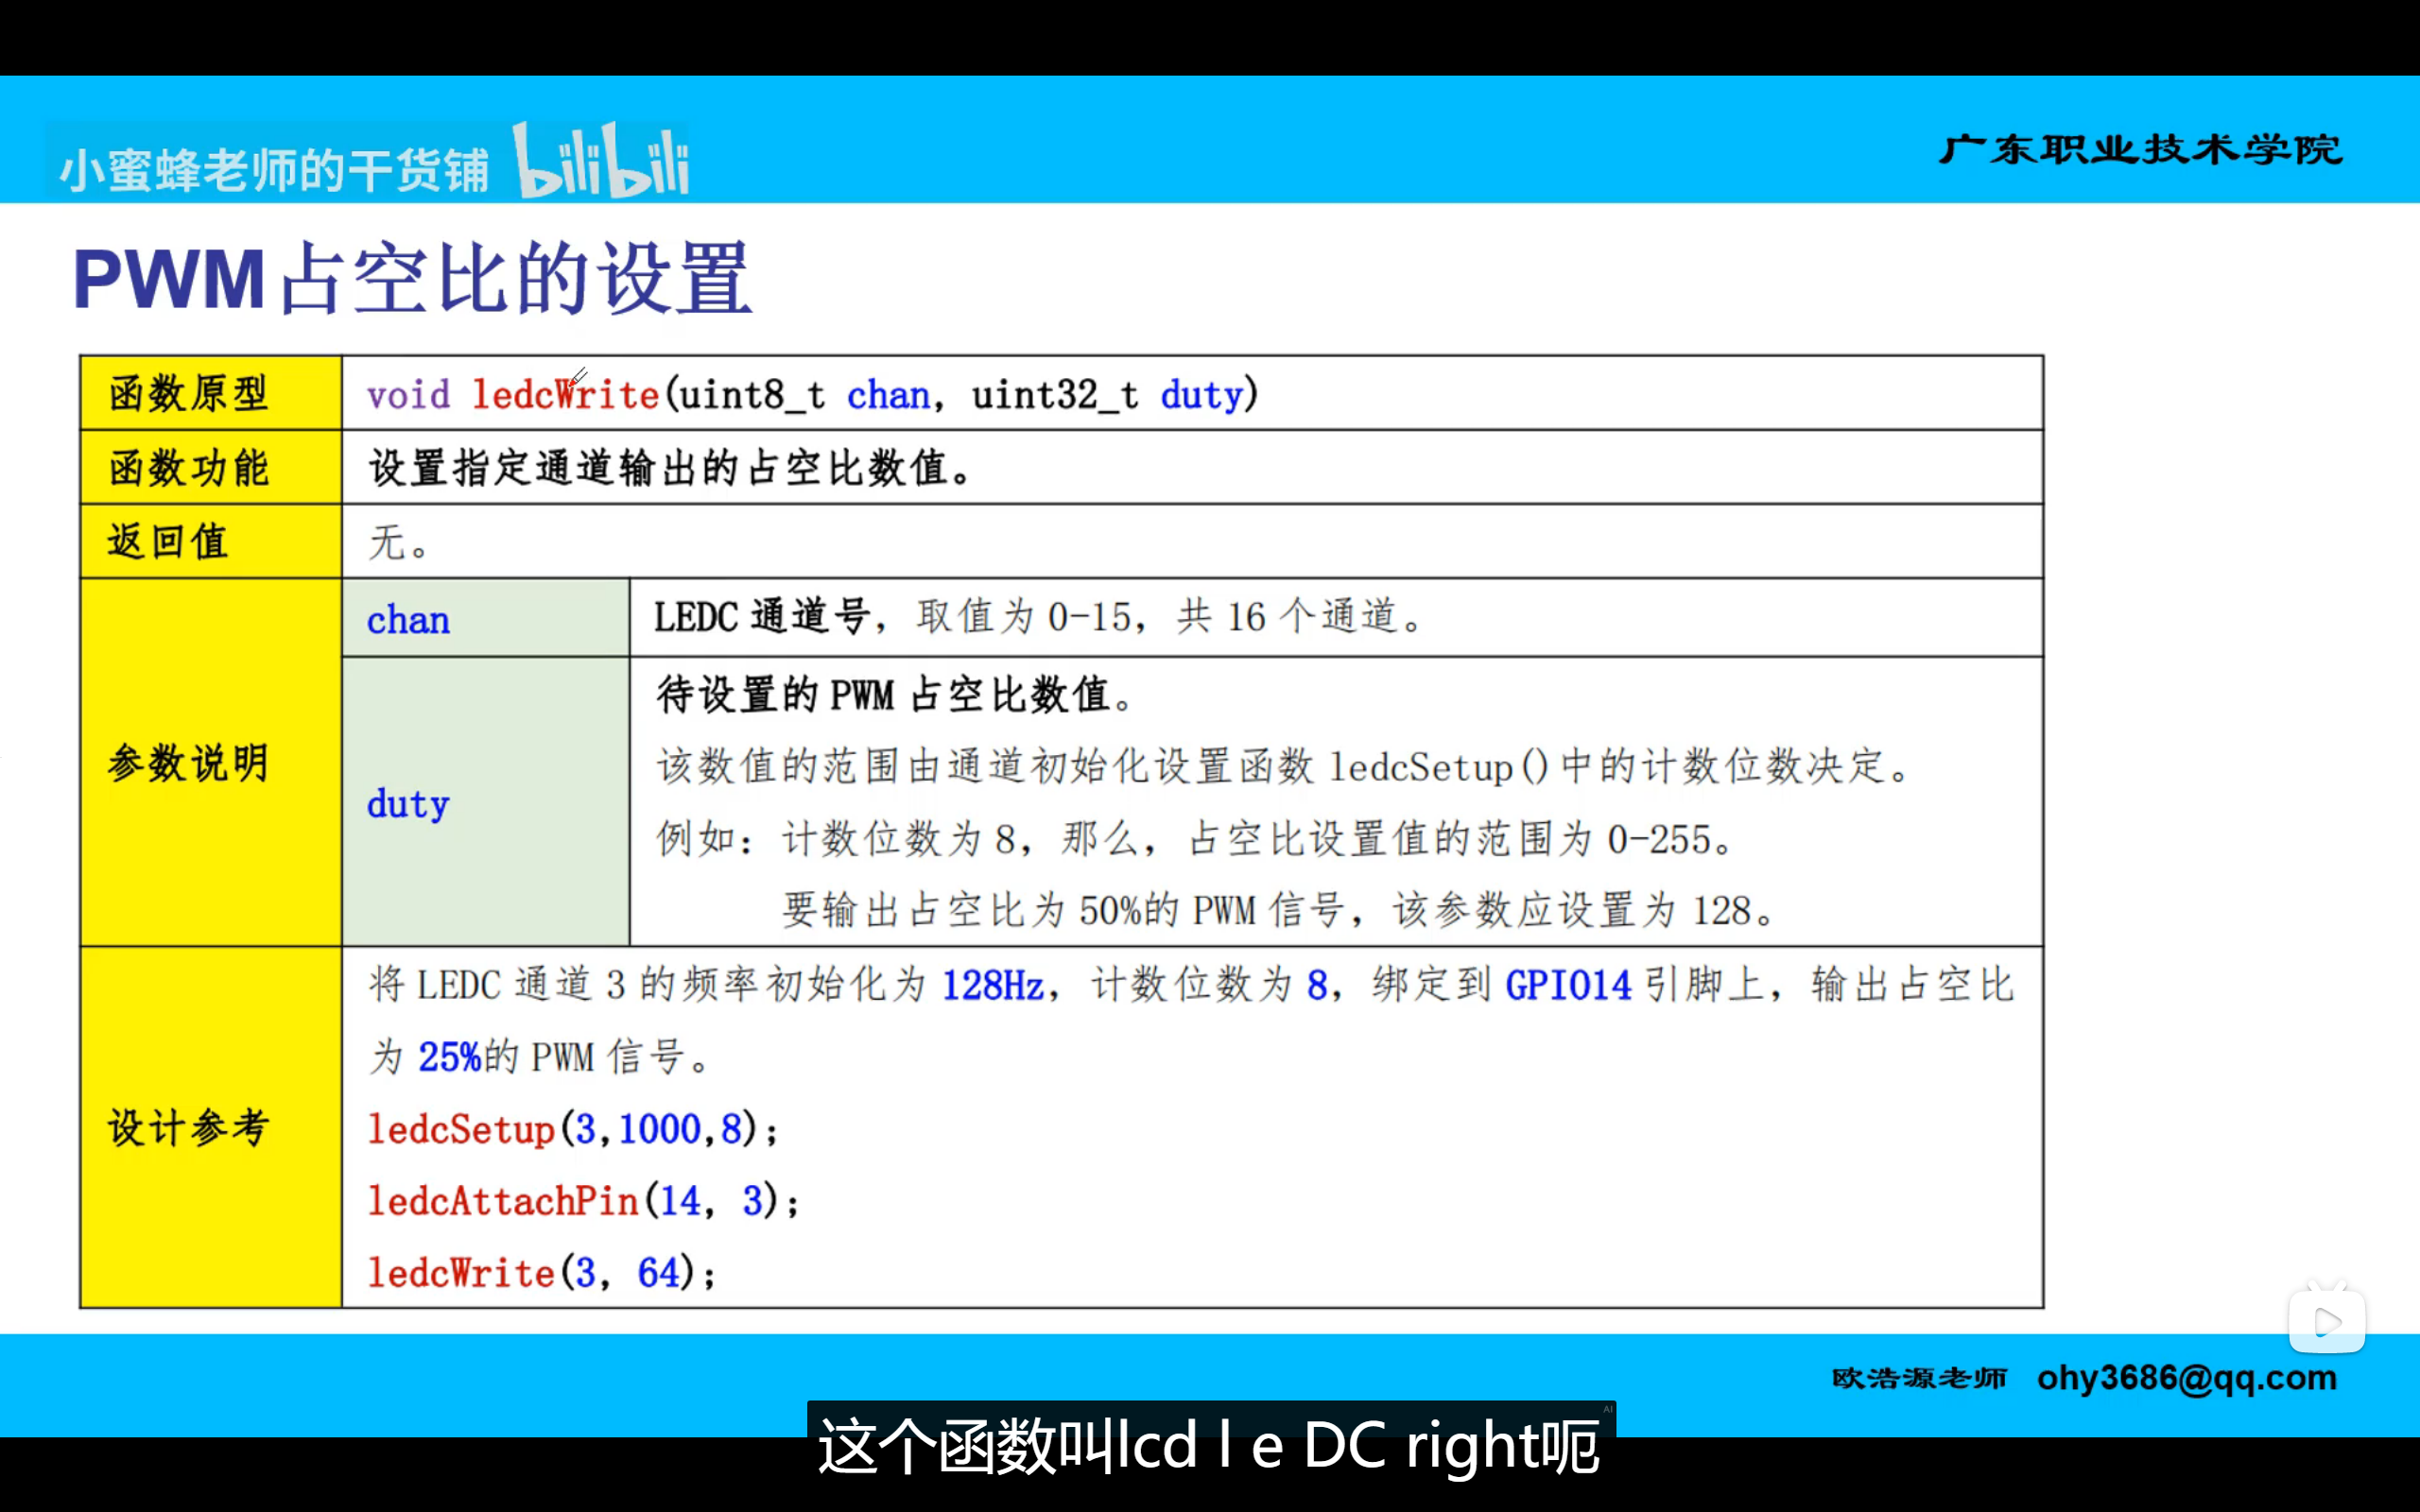
\includegraphics[width=\textwidth]{Figures/ledcWrite.png}
    \caption{ledcWrite}    
\end{figure}
\section{ 串口调试相关函数 }
\subsection{ 串口初始化函数 }
\begin{figure}[h]
    \centering
    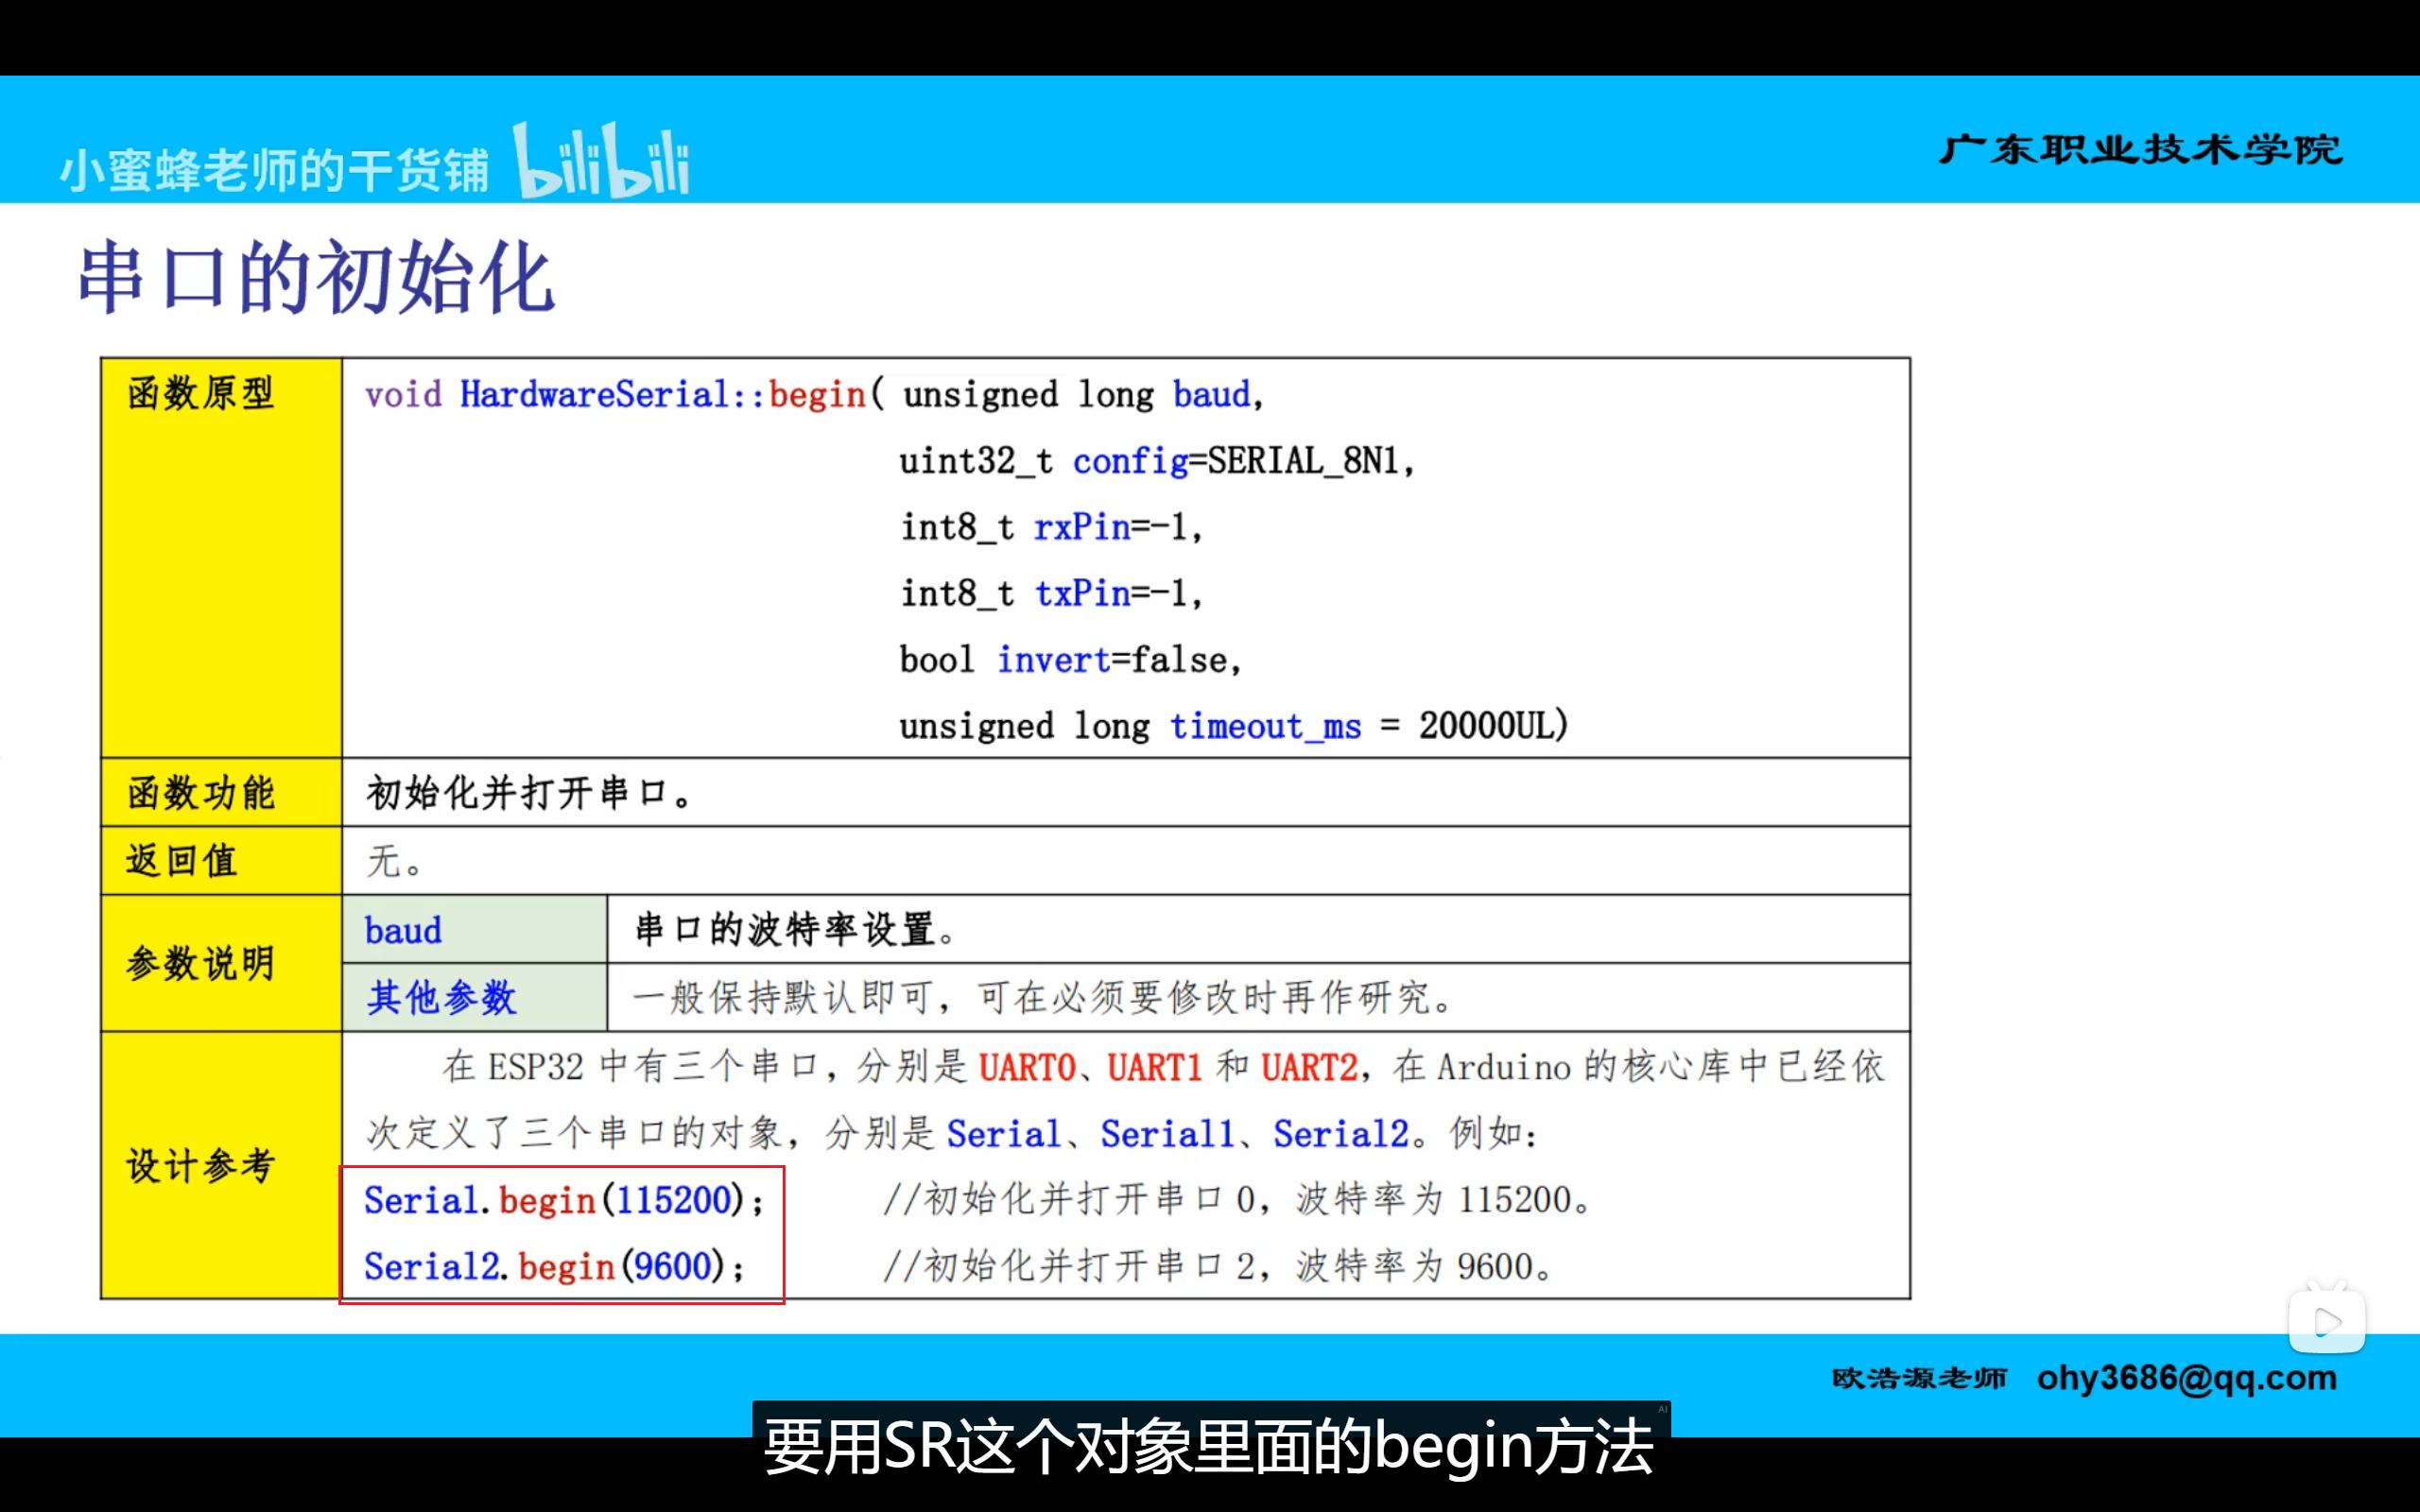
\includegraphics[width=\textwidth]{Figures/Serial.png}
    \caption{Serial}
\end{figure}
函数原型为: \textit{ \textbf{void HardwareSerial::begin} },它有四个参数,第一个参数为要设置的波特率;第二个参数指定串口的数据帧格式，类型为 \textbf{uint32\_t}，默认值为\textbf{ SERIAL\_8N1};
第三第四个参数分别为要重映射的Tx、Rx引脚
\par
在使用时,其实只需要使用\textit{\textbf{Serial.begin,Serial1.begin,Serial.begin}},分别表示\textbf{UART0,UART1,UART2};在设置参数时,大多数情况下只需要设置第一个参数波特率即可
\newpage
\subsection{ 串口打印函数 }
\begin{figure}[h]
    \centering
    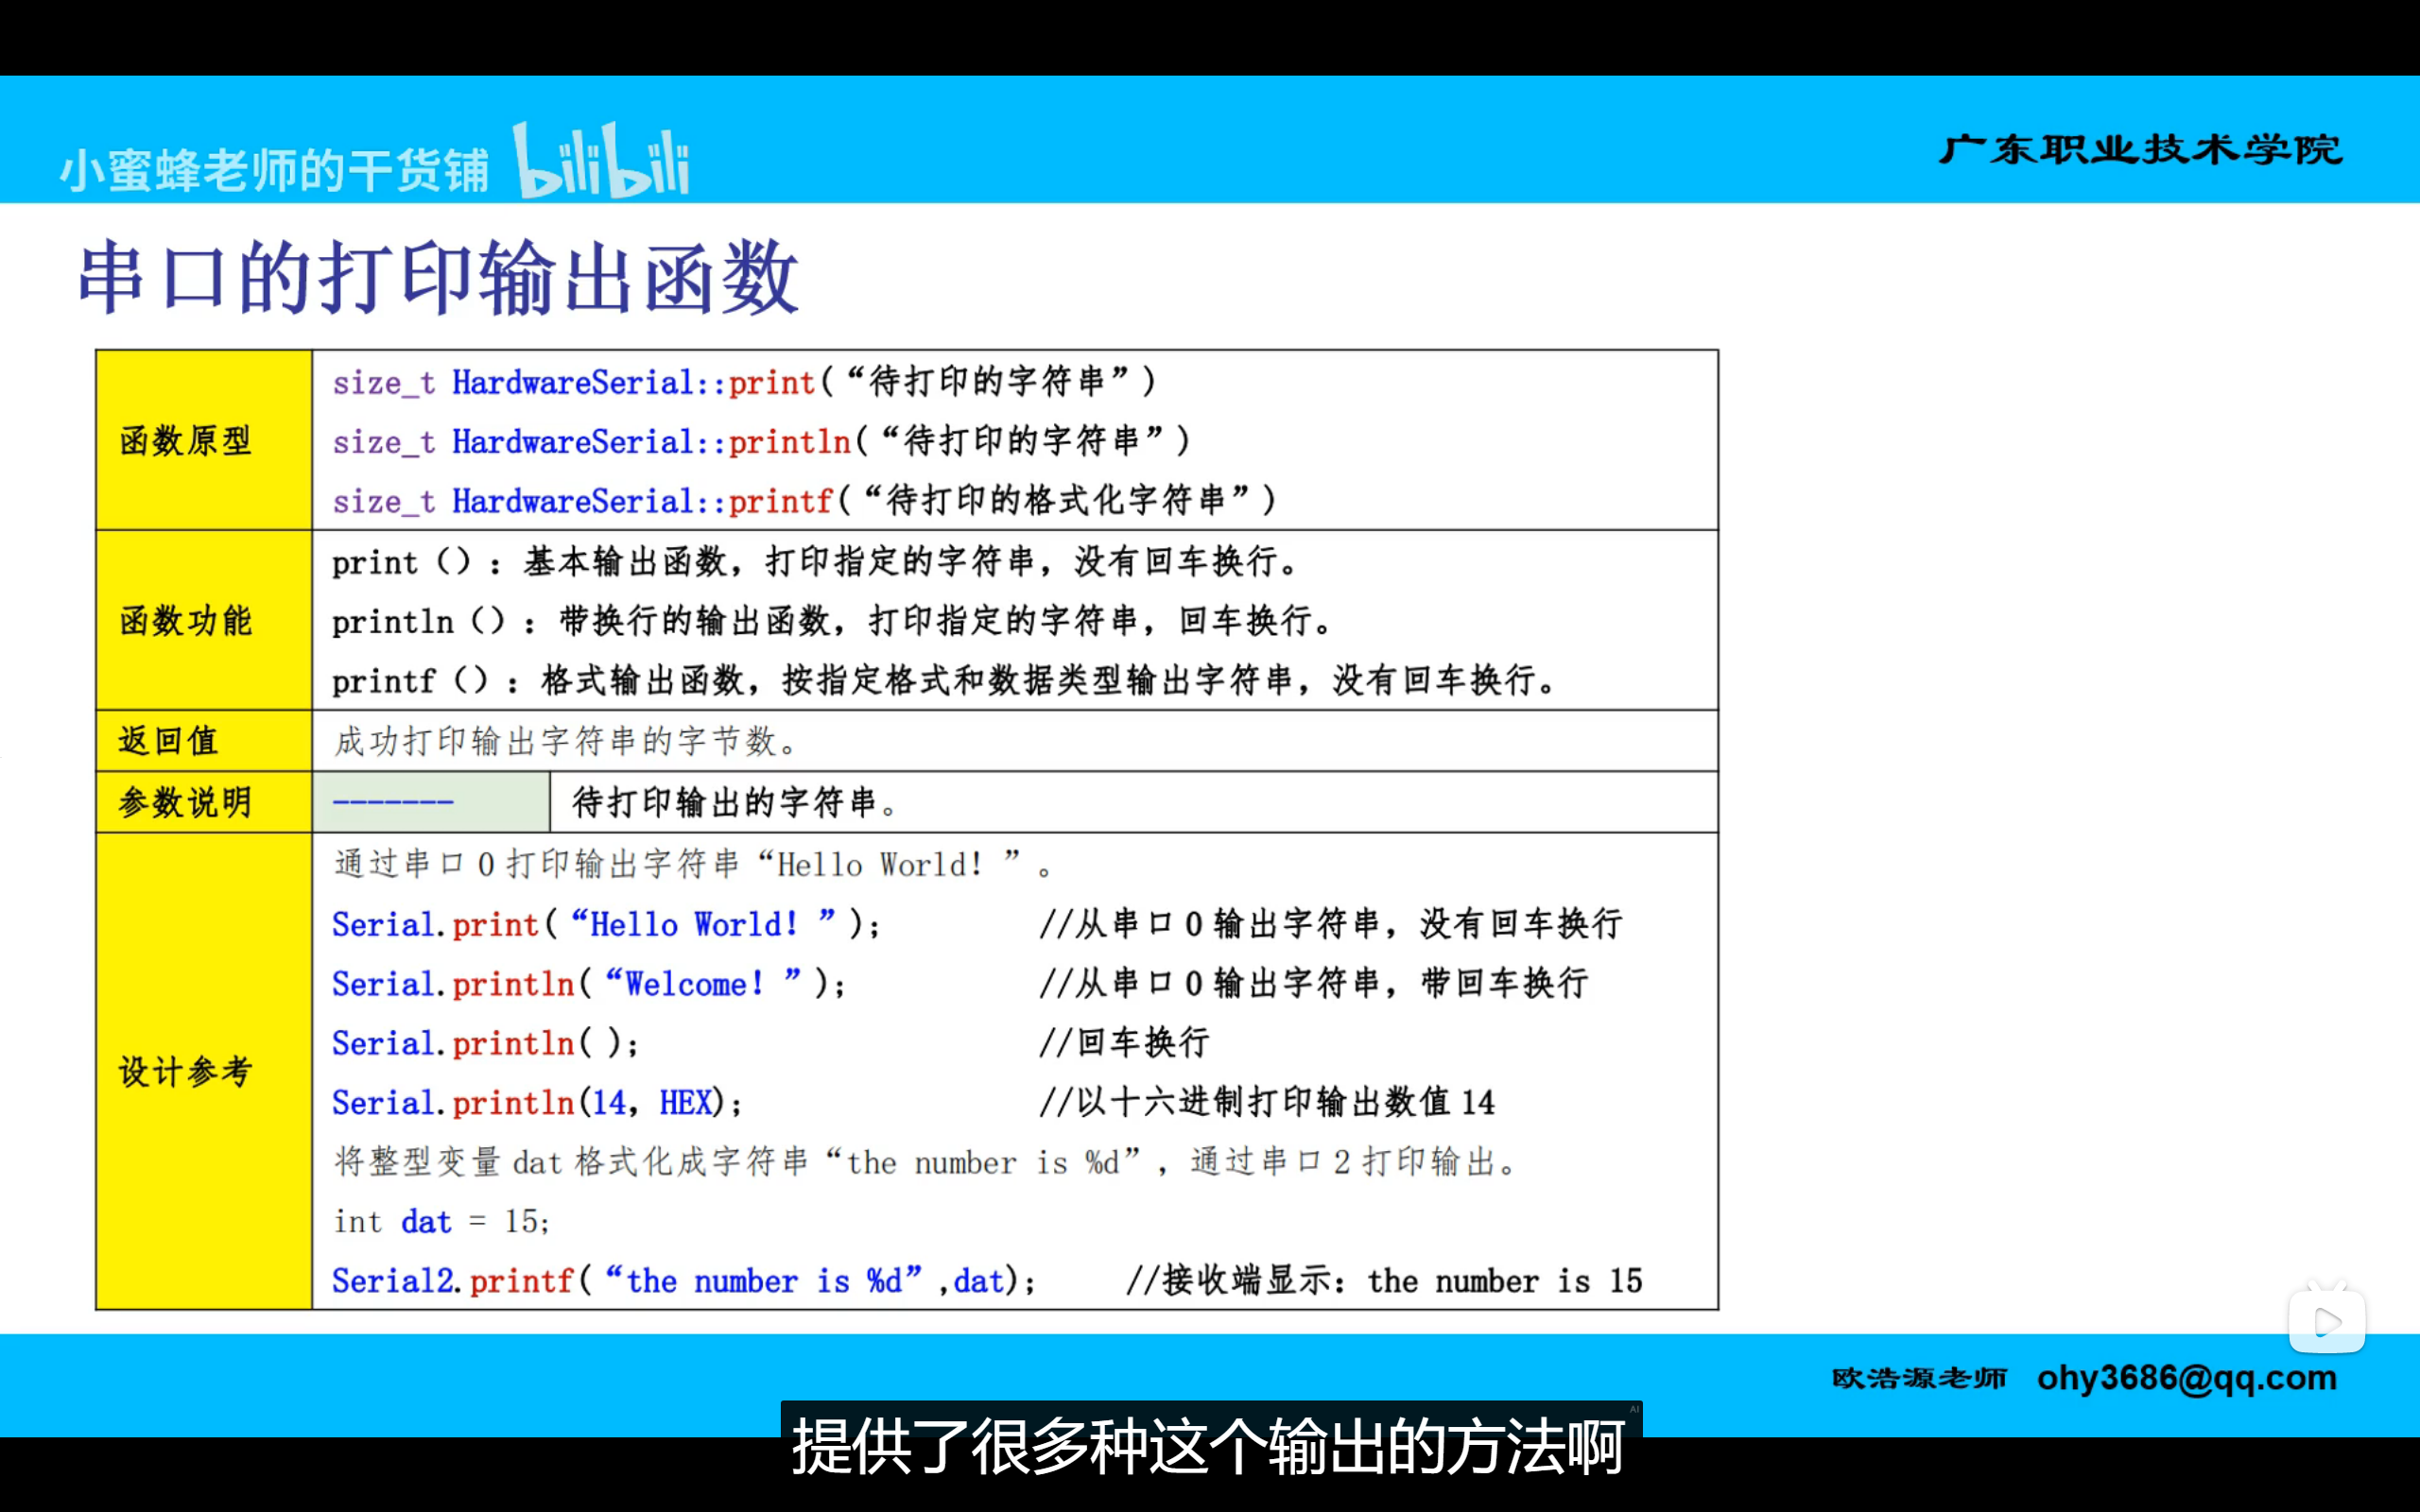
\includegraphics[width=\textwidth]{Figures/Serial_Print.png}
    \caption{Serial打印函数}
\end{figure}
这些函数和上述所说的串口初始化函数用法相似,在实际使用的时候亦是使用\textbf{Serial}(后面添1或者2,不加任何东西表示使用USART0)\textbf{.功能函数名}
\subsection{ 单字符串口写入/读取函数 }
\begin{itemize}
    \item \textit{\textbf{ Serial.write(uint8\_t c) }}:单字符写入
    \item \textit{\textbf{ Serial.read(void)}}:单字符读取
    \item  \textit{\textbf{Serial.available(void)}}:返回该Serial串口缓存区中所有字节的长度
\end{itemize}
\textbf{注意:}
\begin{itemize}
    \item 每个Serial后面都可以加1或2,表示用特定的Serial,不加任何数字表示使用USART0
    \item write、read都是重载函数,即可以往这些函数填入多个参数,根据填入参数数量的不同,函数的功能会发生相应的变化(在下一节中将提到)
\end{itemize}


\newpage
\subsection{ 字符串写入/读取函数(多字符) }
\begin{itemize}
    \item 字符串写入函数(单片机给电脑发送消息):Serial.write(参数一,参数二).参数一为要读取数据的地址(数组名或者指针);参数二为要读取数据的长度.
    \item  字符串读取函数(读取电脑给单片机发送的消息):Serial.read(参数一,参数二).参数一表示要把数据存储到哪个数组(同上),参数二为要读取的长度
\end{itemize}
\par
在读取函数的代码实现中,我们一般先定义一个变量(假设为a),将Serial.available()返回的数据长度赋值给a.这样a就可以作为Serial.read的第二个参数了(表示把缓存区里面的数据全部读取出来). 两个函数具体如下:
\begin{figure}[h]
    \begin{minipage}{0.48\textwidth}
        \centering
        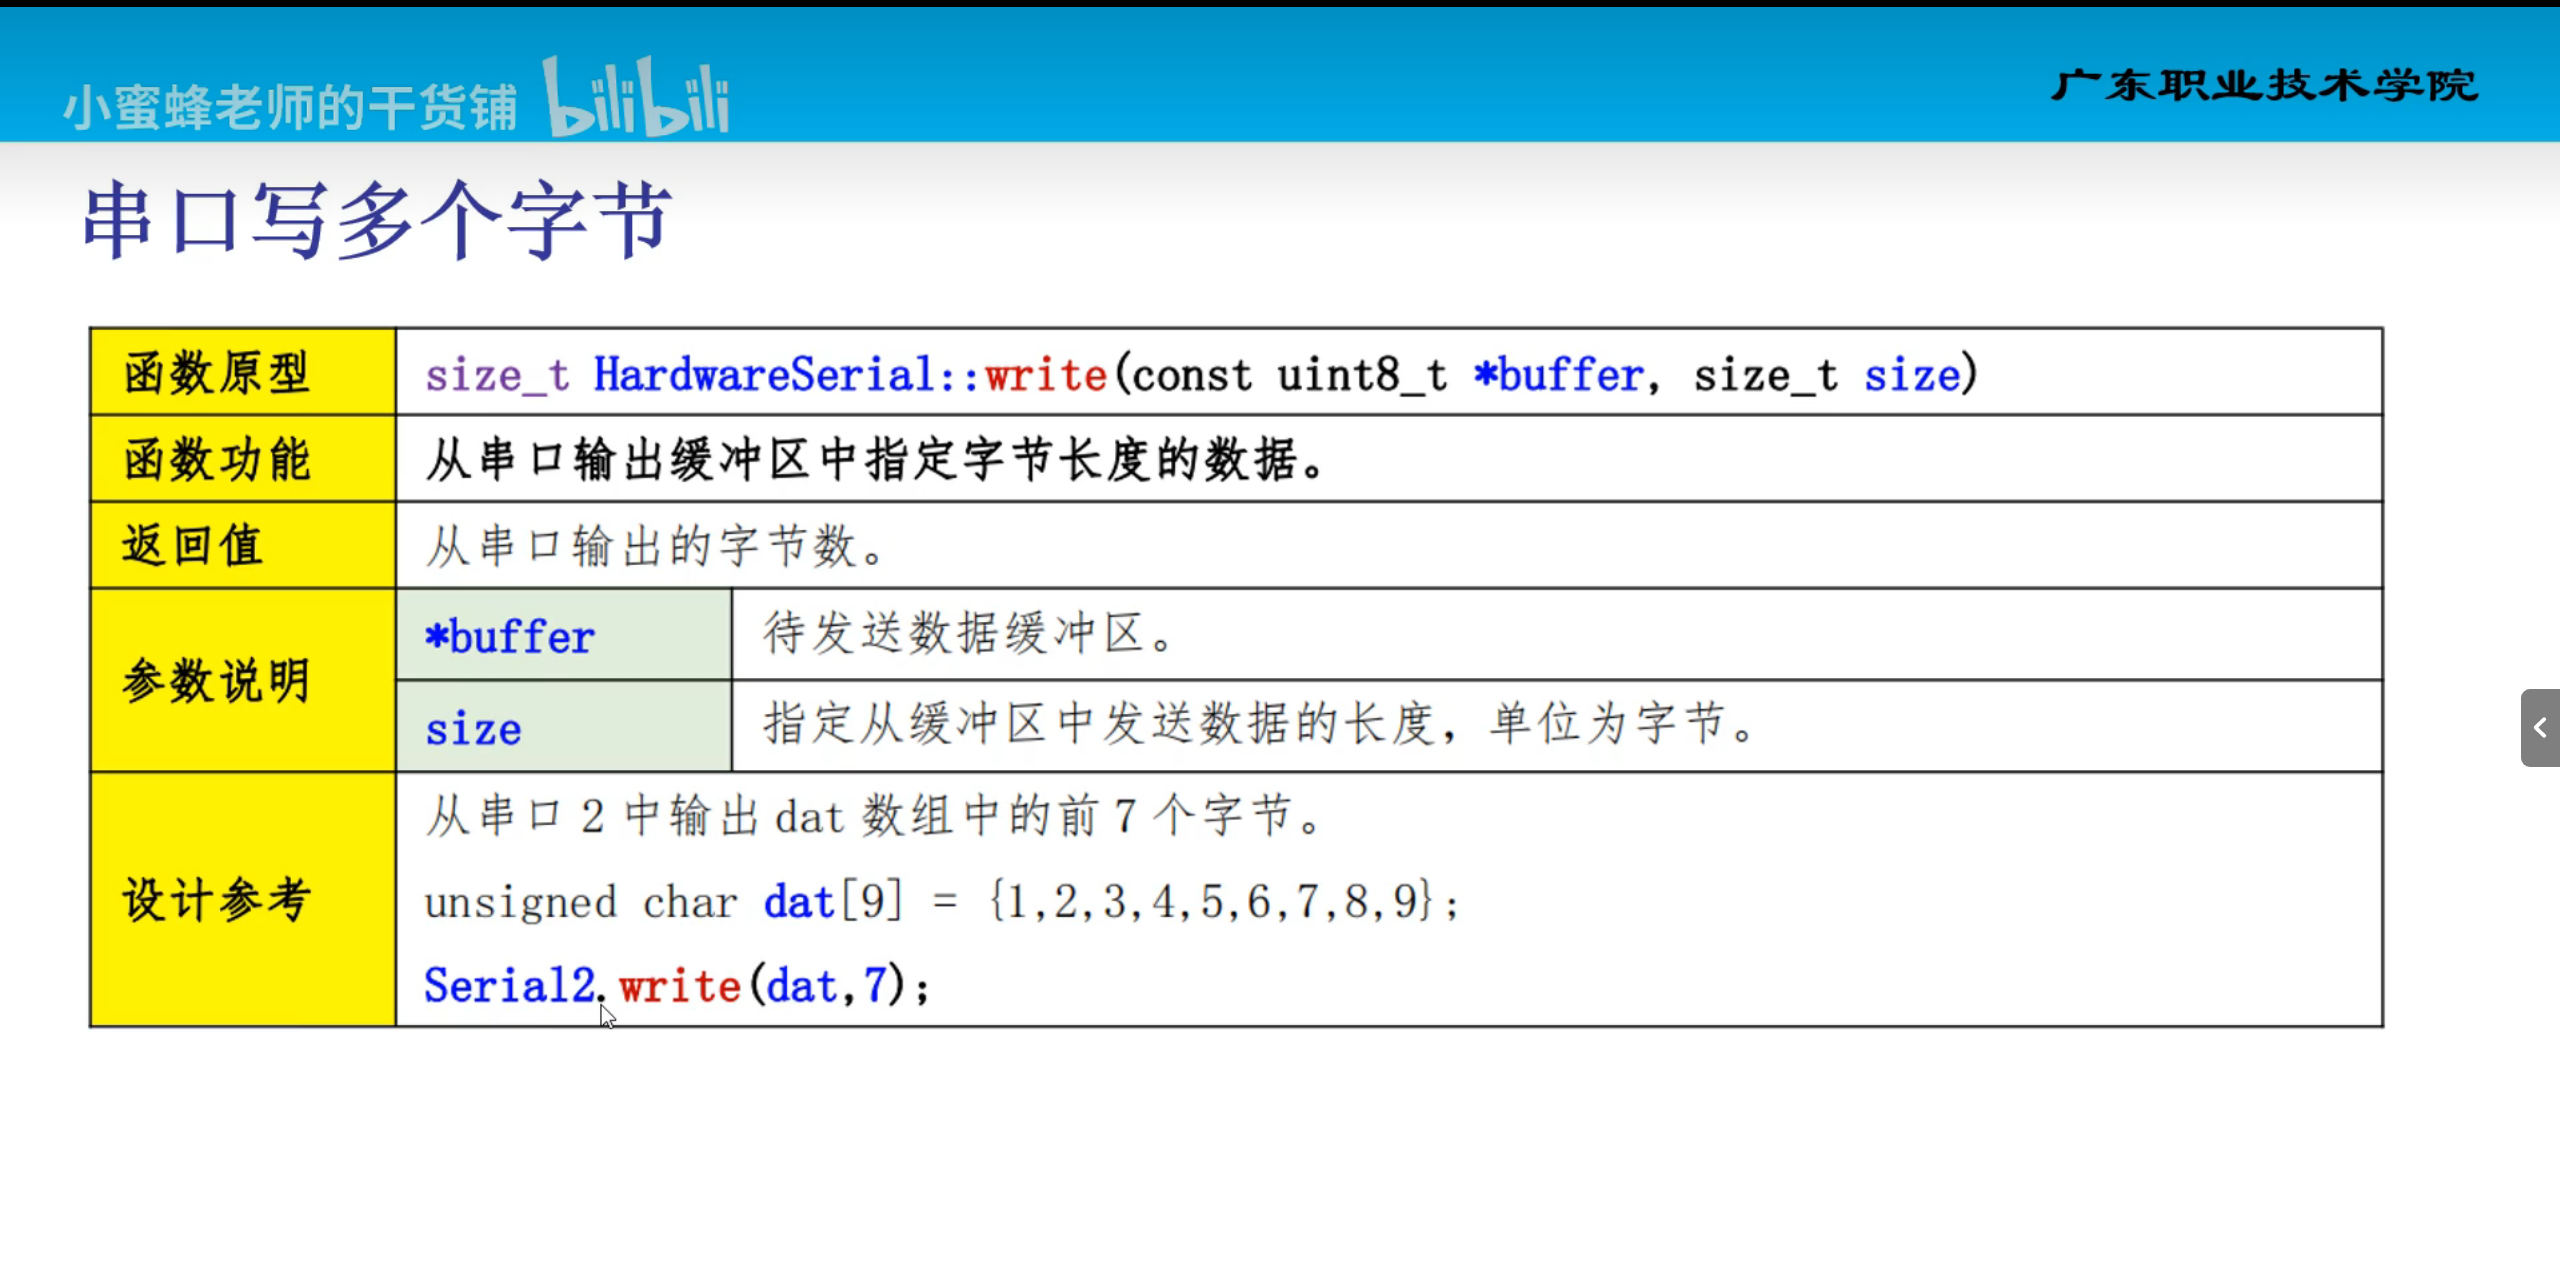
\includegraphics[width = 0.8\textwidth]{Figures/Serial-write.png}
        \caption{Serial.write}
    \end{minipage}
    \begin{minipage}{0.48\textwidth}
        \centering
        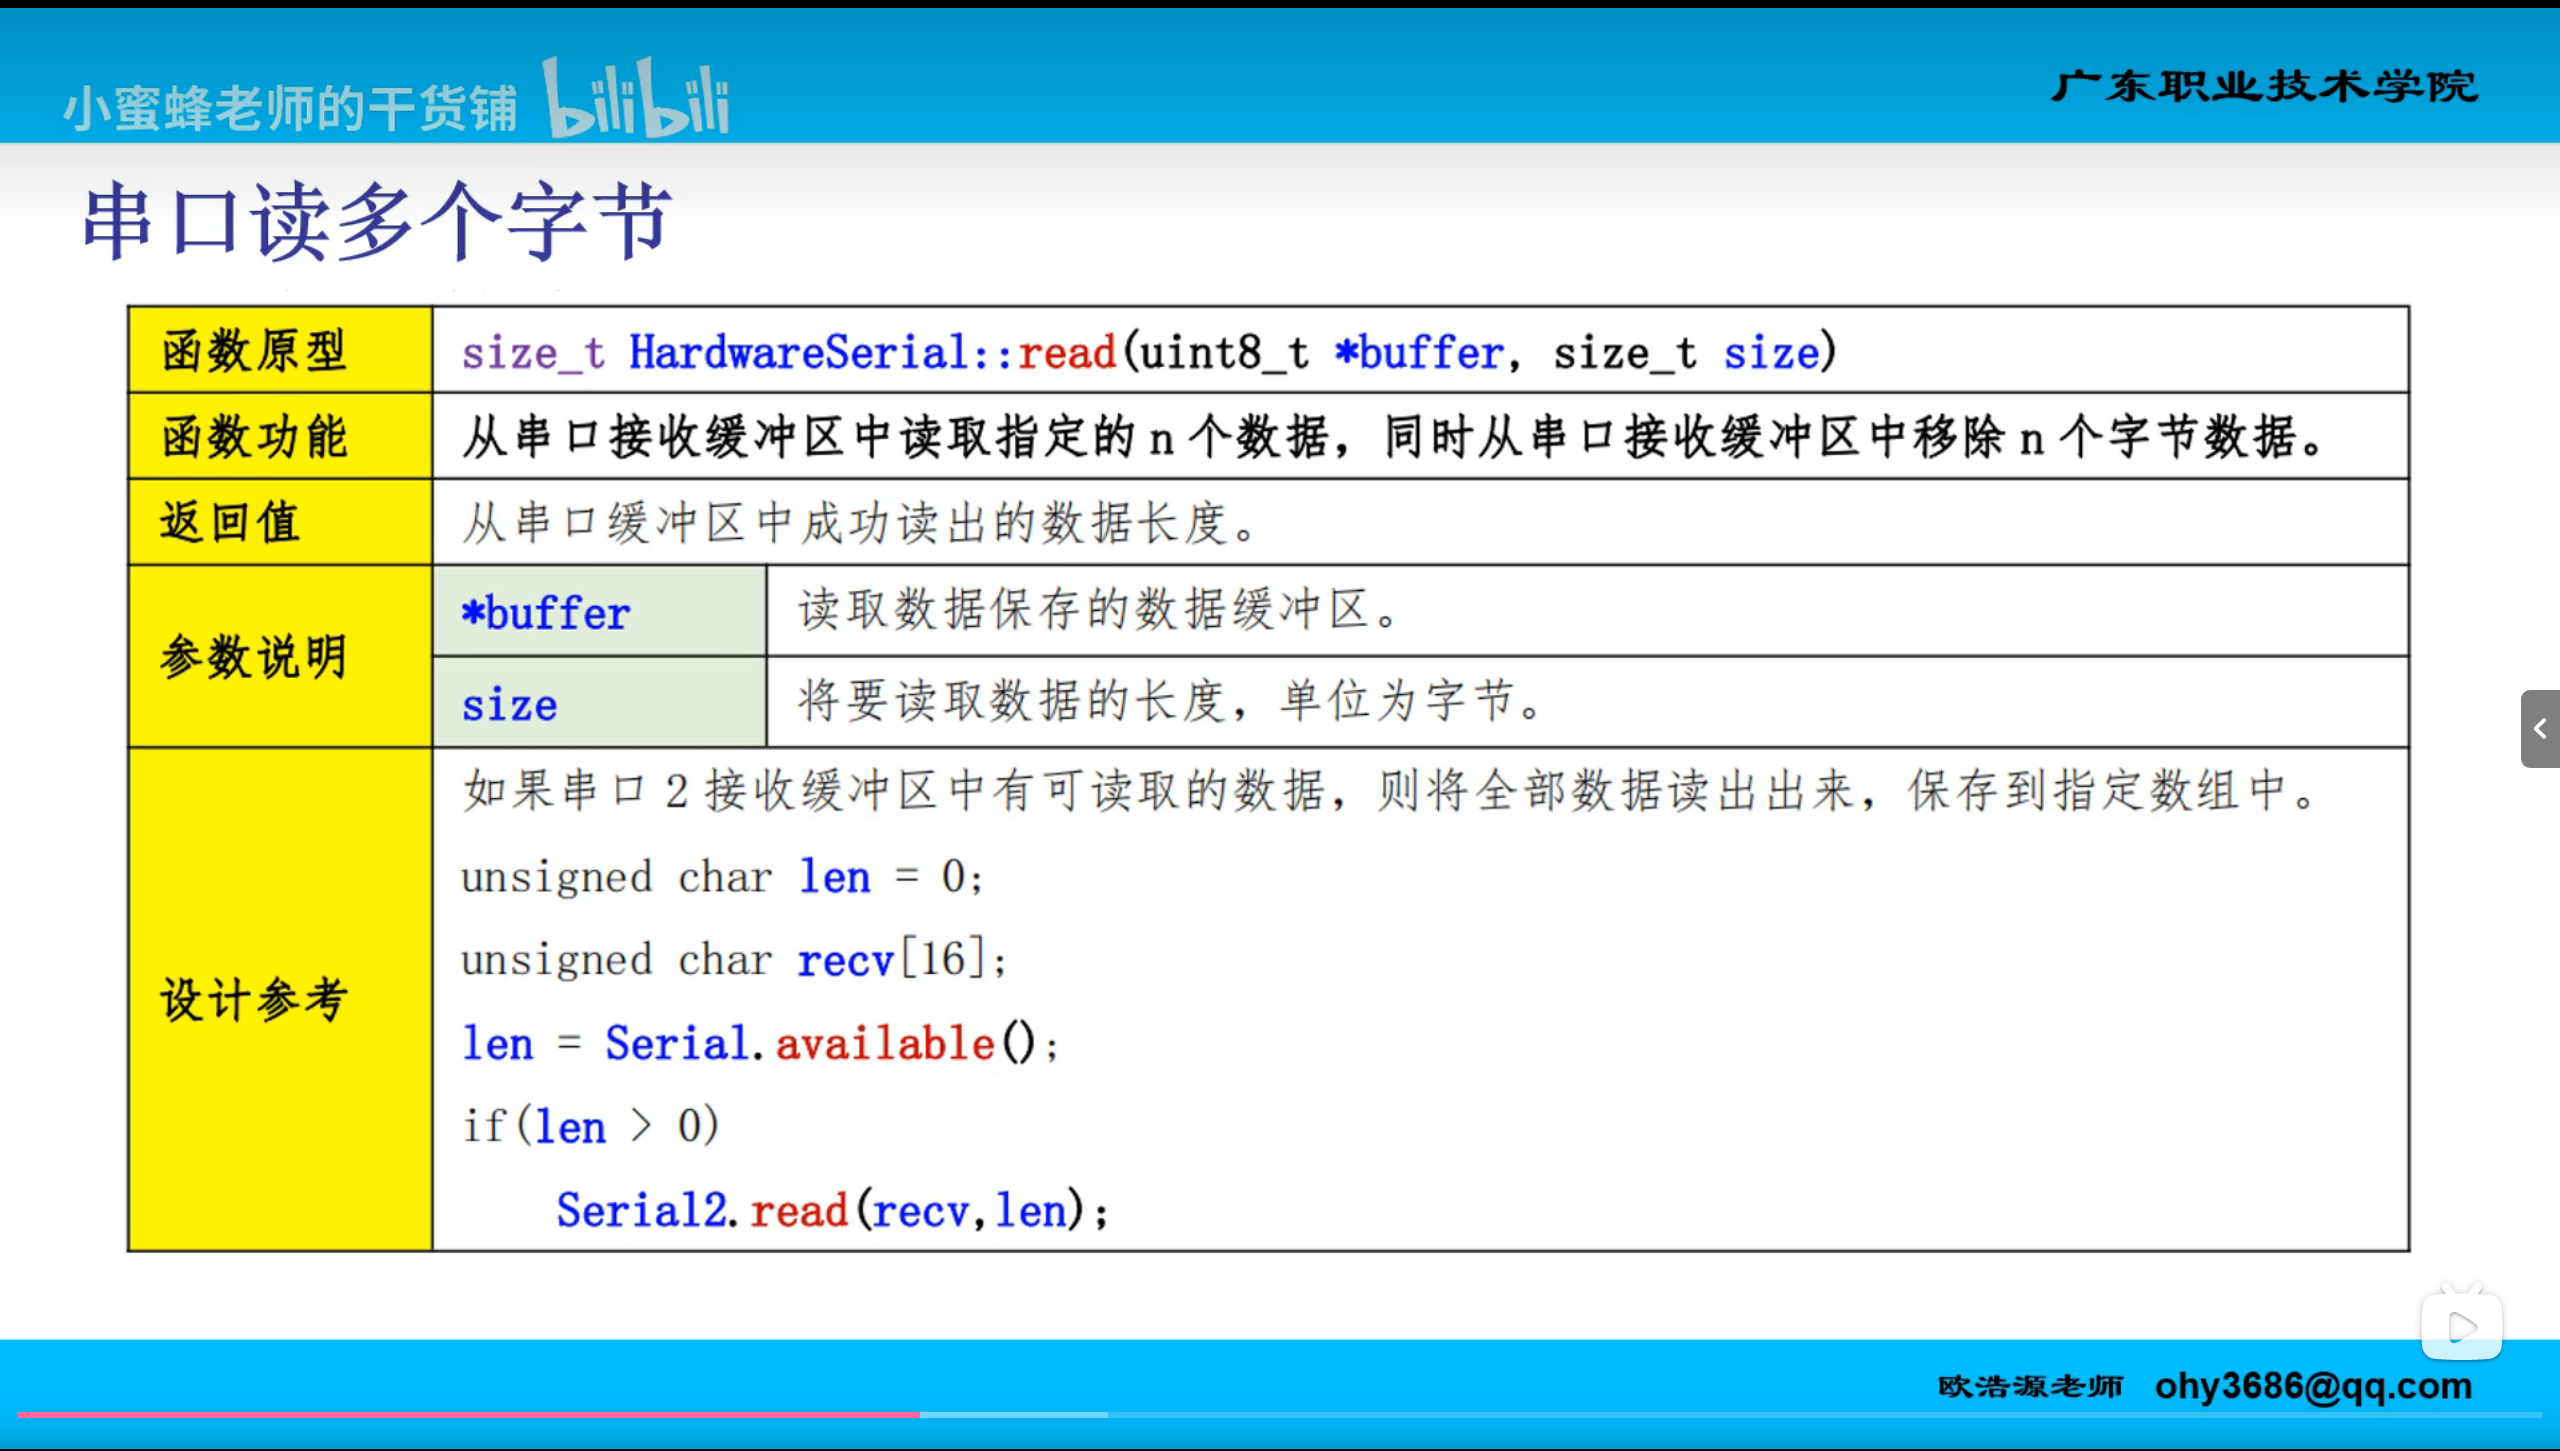
\includegraphics[width = 0.8\textwidth]{Figures/Serial-read.png}
        \caption{Serial.read}
    \end{minipage}
        
    
\end{figure}
\subsection{ 使用串口时注意的事项 }
如果在用USART0进行调试时遇到无法接收任何消息,但是又没有报错的情况,那么可以去platformio.ini文件里面增加这几段代码:
\begin{verbatim}
monitor_speed = 115200
monitor_port = COM7
upload_port = COM7
build_flags =
    -DARDUINO_USB_MODE=1
    -DARDUINO_USB_CDC_ON_BOOT=0
\end{verbatim}
\newpage
如图所示:
\begin{figure}[h]
    \centering
    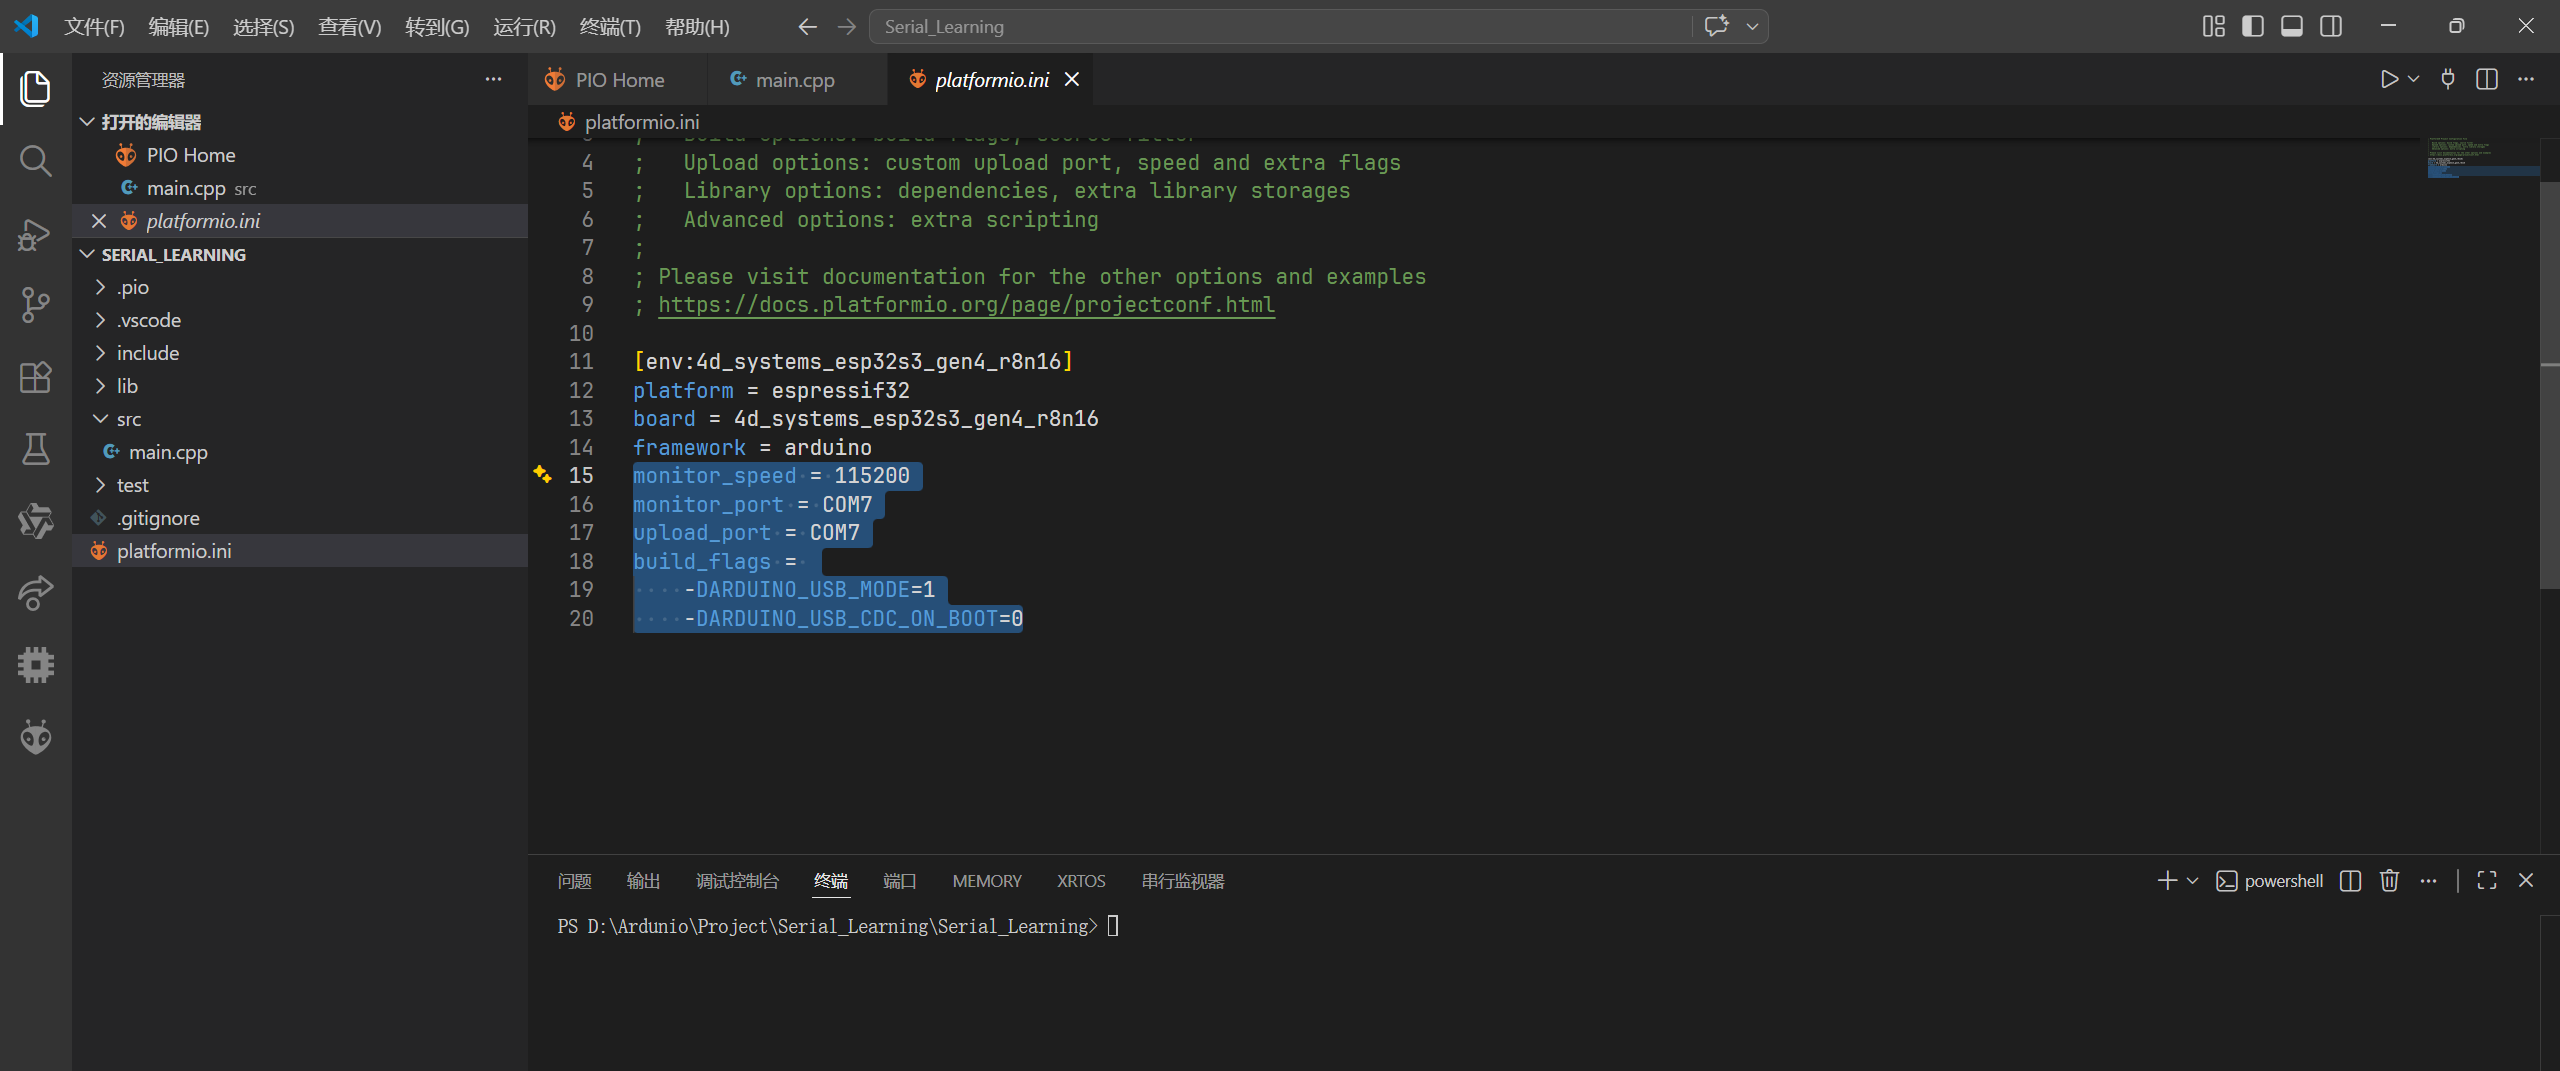
\includegraphics[width=\textwidth]{Figures/System_Build_Structure.png}
    \caption{Caption}
    \label{fig:placeholder}
\end{figure}
\par
这几段代码的作用分别为:
\begin{itemize}
    \item monitor\_speed：设置串口波特率。
    \item monitor\_port / upload\_port：指定使用 COM7，避免自动检测错误。
    \item -DARDUINO\_USB\_MODE=1：禁用原生 USB CDC，串口走 UART0（CH343）。
    \item -DARDUINO\_USB\_CDC\_ON\_BOOT=0：启动时不初始化 USB CDC，确保 Serial 映射到 UART0。
\end{itemize}

\noindent
\par
总结：  
默认情况下，Serial 被映射到原生 USB CDC，而硬件连接的是 CH343（UART 转 USB）。两者不匹配导致无法接收数据。通过上述配置，将 Serial 强制映射到 UART0，从而恢复通信。
\section{ 与中断相关的知识点 }
\subsection{ 中断开启和关闭函数 }
\begin{itemize}
    \item 中断开启函数:void attachInterrupt(参数一,参数二,参数三).参数一表示要为哪一个引脚开启中断;参数二表示中断触发时要调用哪个函数(填入函数指针);参数三为触发中断的方式
        \begin{table}[h]
    \centering
    \begin{tabular}{|l|l|}
    \hline
    \textbf{宏定义} & \textbf{含义} \\
    \hline
    \texttt{RISING}  & 上升沿触发（低$\rightarrow$高） \\
    \hline
    \texttt{FALLING} & 下降沿触发（高$\rightarrow$低） \\
    \hline
    \texttt{CHANGE}  & 电平变化时触发 \\
    \hline
    \texttt{LOW}     & 低电平触发 \\
    \hline
    \texttt{HIGH}    & 高电平触发（ESP32支持，Arduino Uno不支持） \\
    \hline
    \end{tabular}
    \caption{attachInterrupt 触发方式}
    \end{table}
    \item 中断关闭函数:void detachInterrupt(参数一),参数一表示要将哪个引脚的中断功能关闭
\end{itemize}
具体说明如下:
\begin{figure}[h]
    \begin{minipage}{0.48\textwidth}
        \centering
        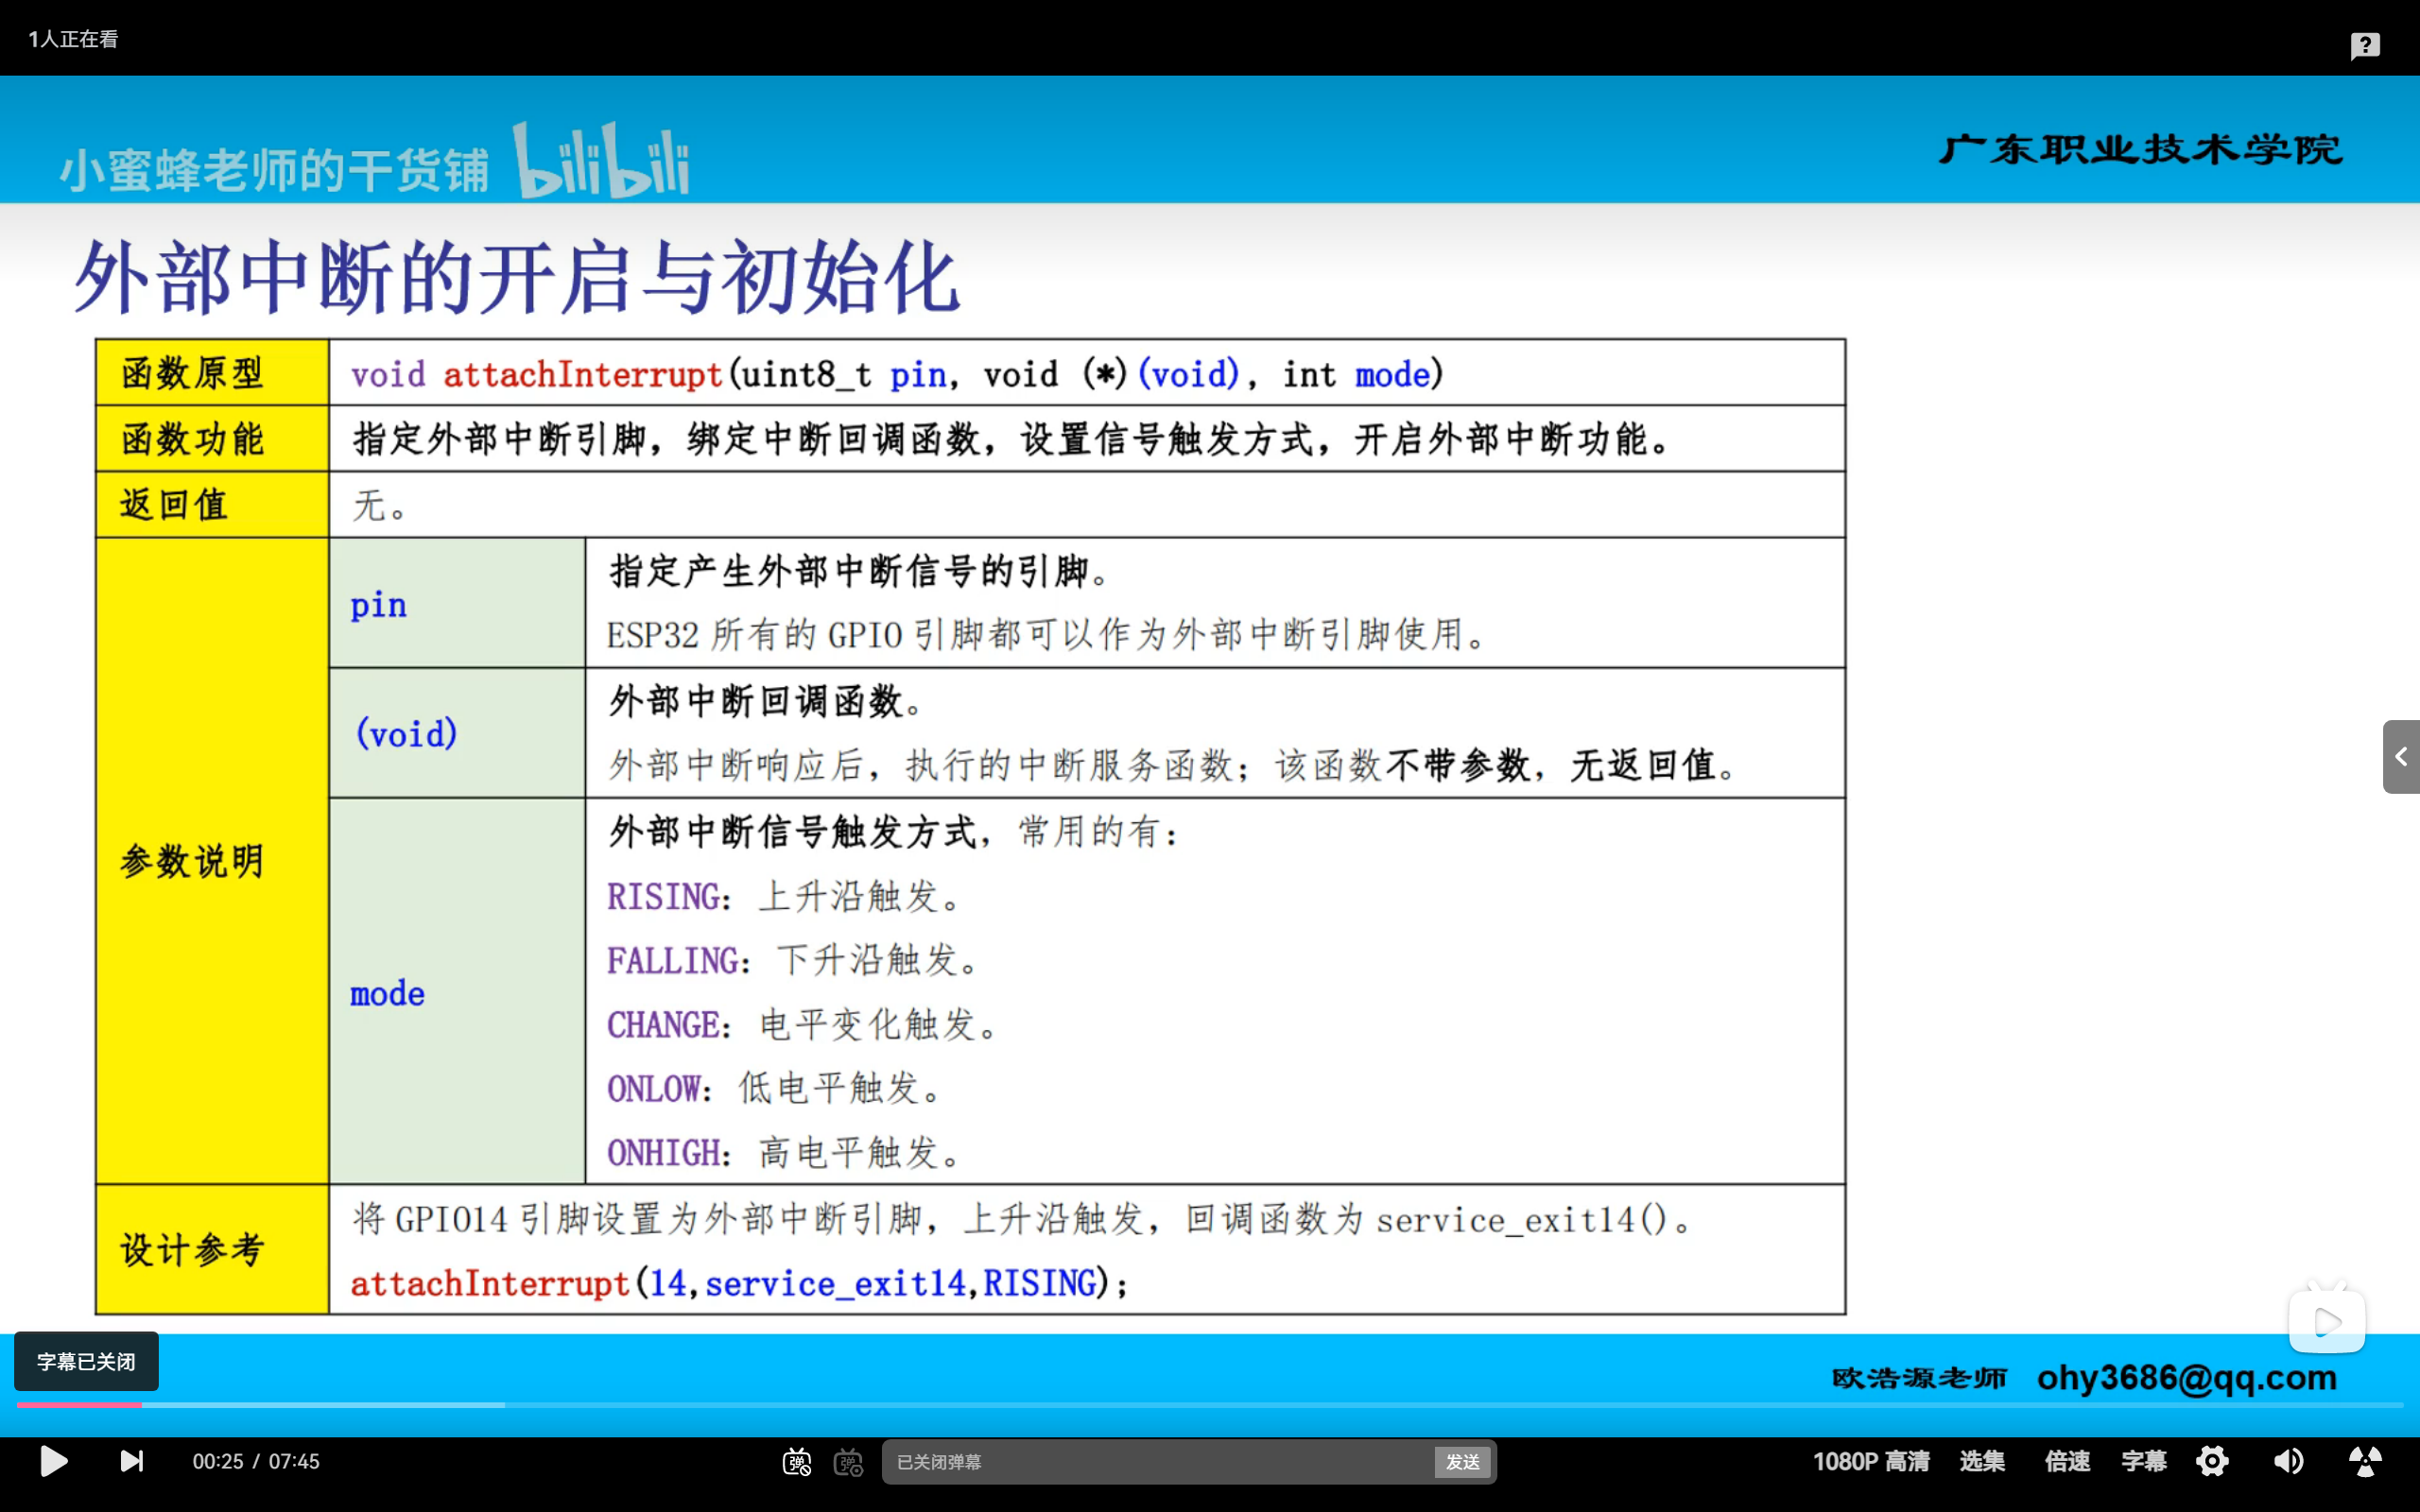
\includegraphics[width = 0.8\textwidth]{Figures/PreInterrupt.png}
        \caption{外部中断开启函数}
    \end{minipage}
    \begin{minipage}{0.48\textwidth}
        \centering
        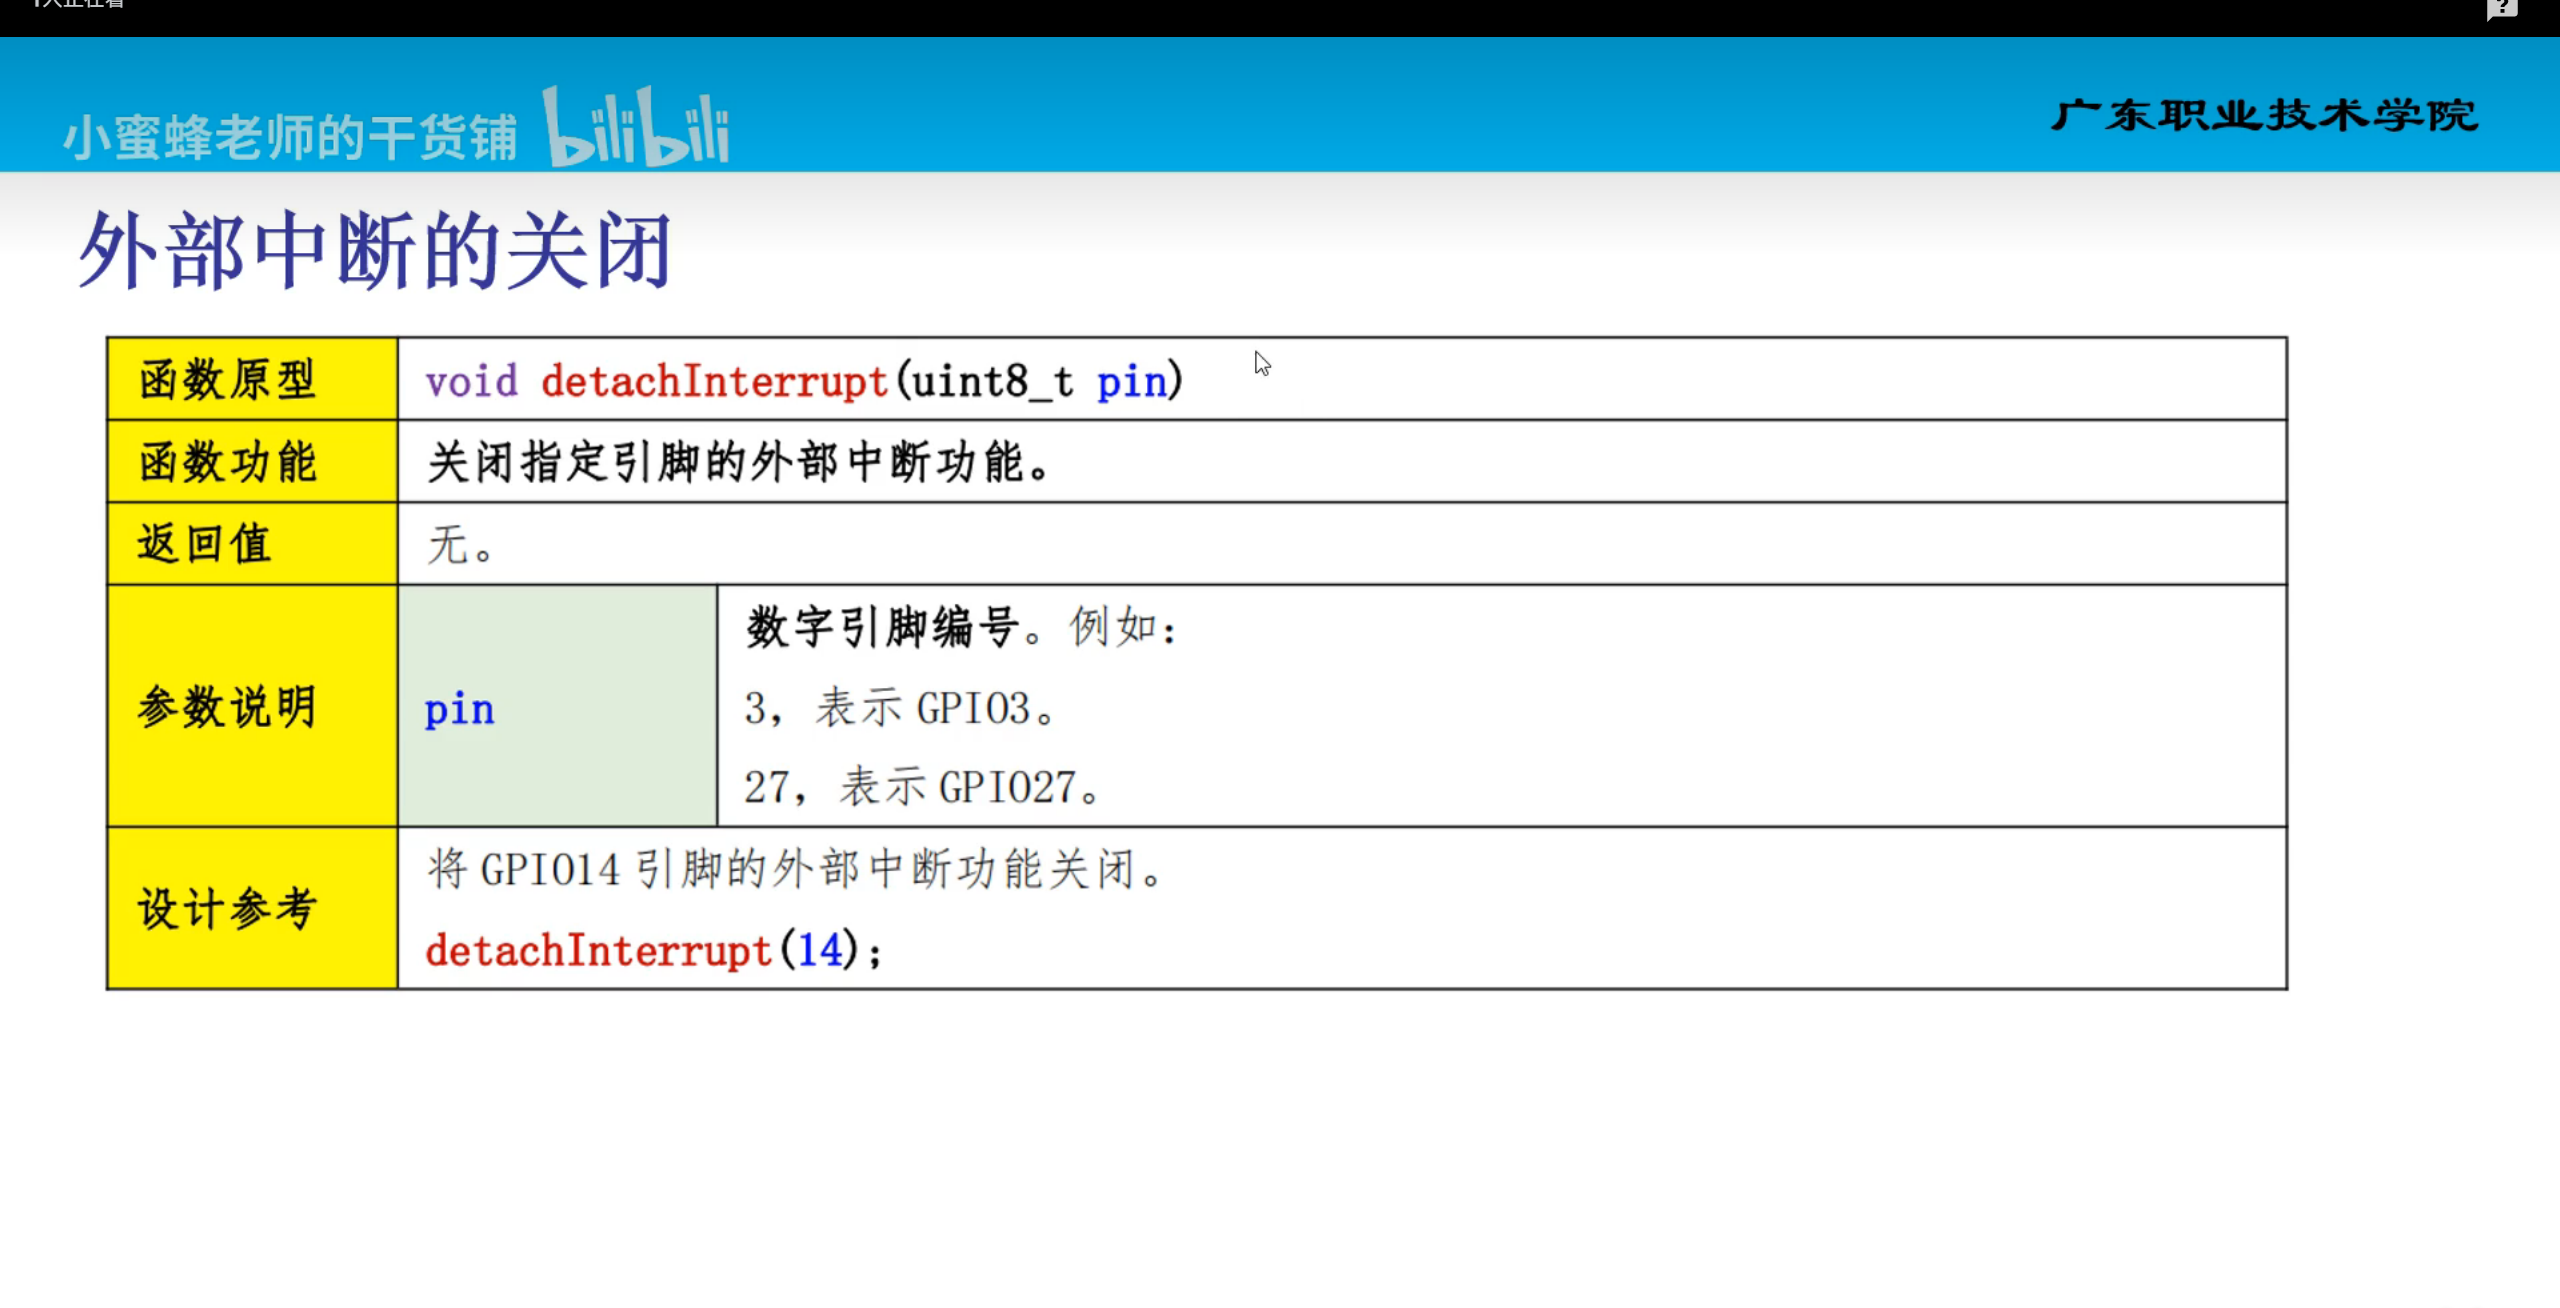
\includegraphics[width = 0.8\textwidth]{Figures/PreInterrupt_Close.png}
        \caption{外部中断关闭函数}
    \end{minipage}
\end{figure}
以下是具体的代码示例:
\begin{figure}[h]
    \centering
    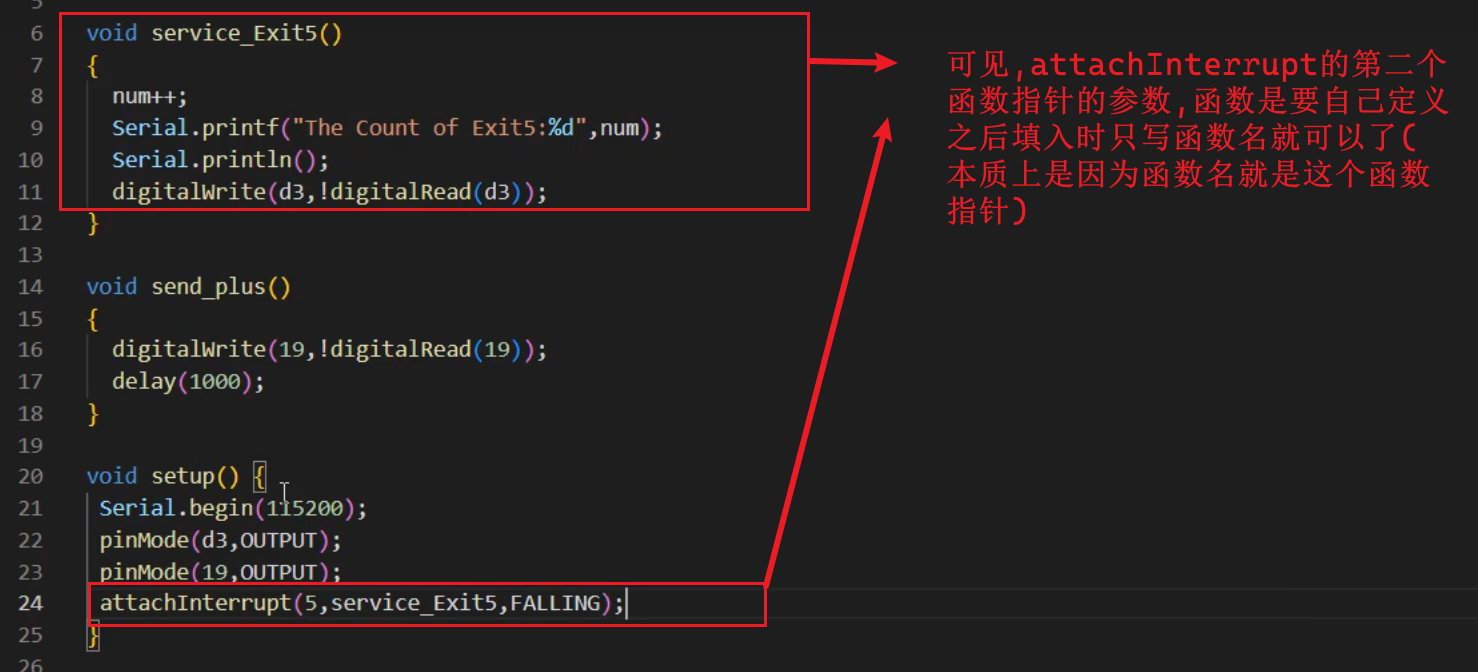
\includegraphics[width=0.5\textwidth]{Figures/Exemple_Code.png}
    \caption{外部中断开启的示例代码}
\end{figure}

\section{ 基于Arduino的定时器库函数}
\subsection{基于Arduino的Timer定时器概述}

ESP32 提供 2 个硬件定时器组，每组有 2 个硬件通用定时器，即 ESP32 芯片内置 4 个硬件通用定时器，分别对应序号：0、1、2、3。

每个定时器包含 1 个 16 位预分频器和 1 个 64 位可自动重载向上/向下计数器。

ESP32 的计数基频为 80\,MHz，预分频系数为 80 可得到 1\,MHz 的计数信号，每个计数信号的周期为 1\,$\mu$s，即每个计数单位为 1\,$\mu$s。

\subsection{定时器的初始化流程}

初始化一个定时器对象：\texttt{timerBegin()}，返回 \texttt{hw\_timer\_t} 类型的定时器对象。

设置定时器中断：\texttt{timerAttachInterrupt()}。

配置定时器参数：\texttt{timerAlarmWrite()}。

使能开启定时器：\texttt{timerAlarmEnable()}。

\subsection{定时器中断回调各函数具体介绍}
\subsubsection{ 定时器初始化函数 }
\begin{figure}[h]
    \centering
    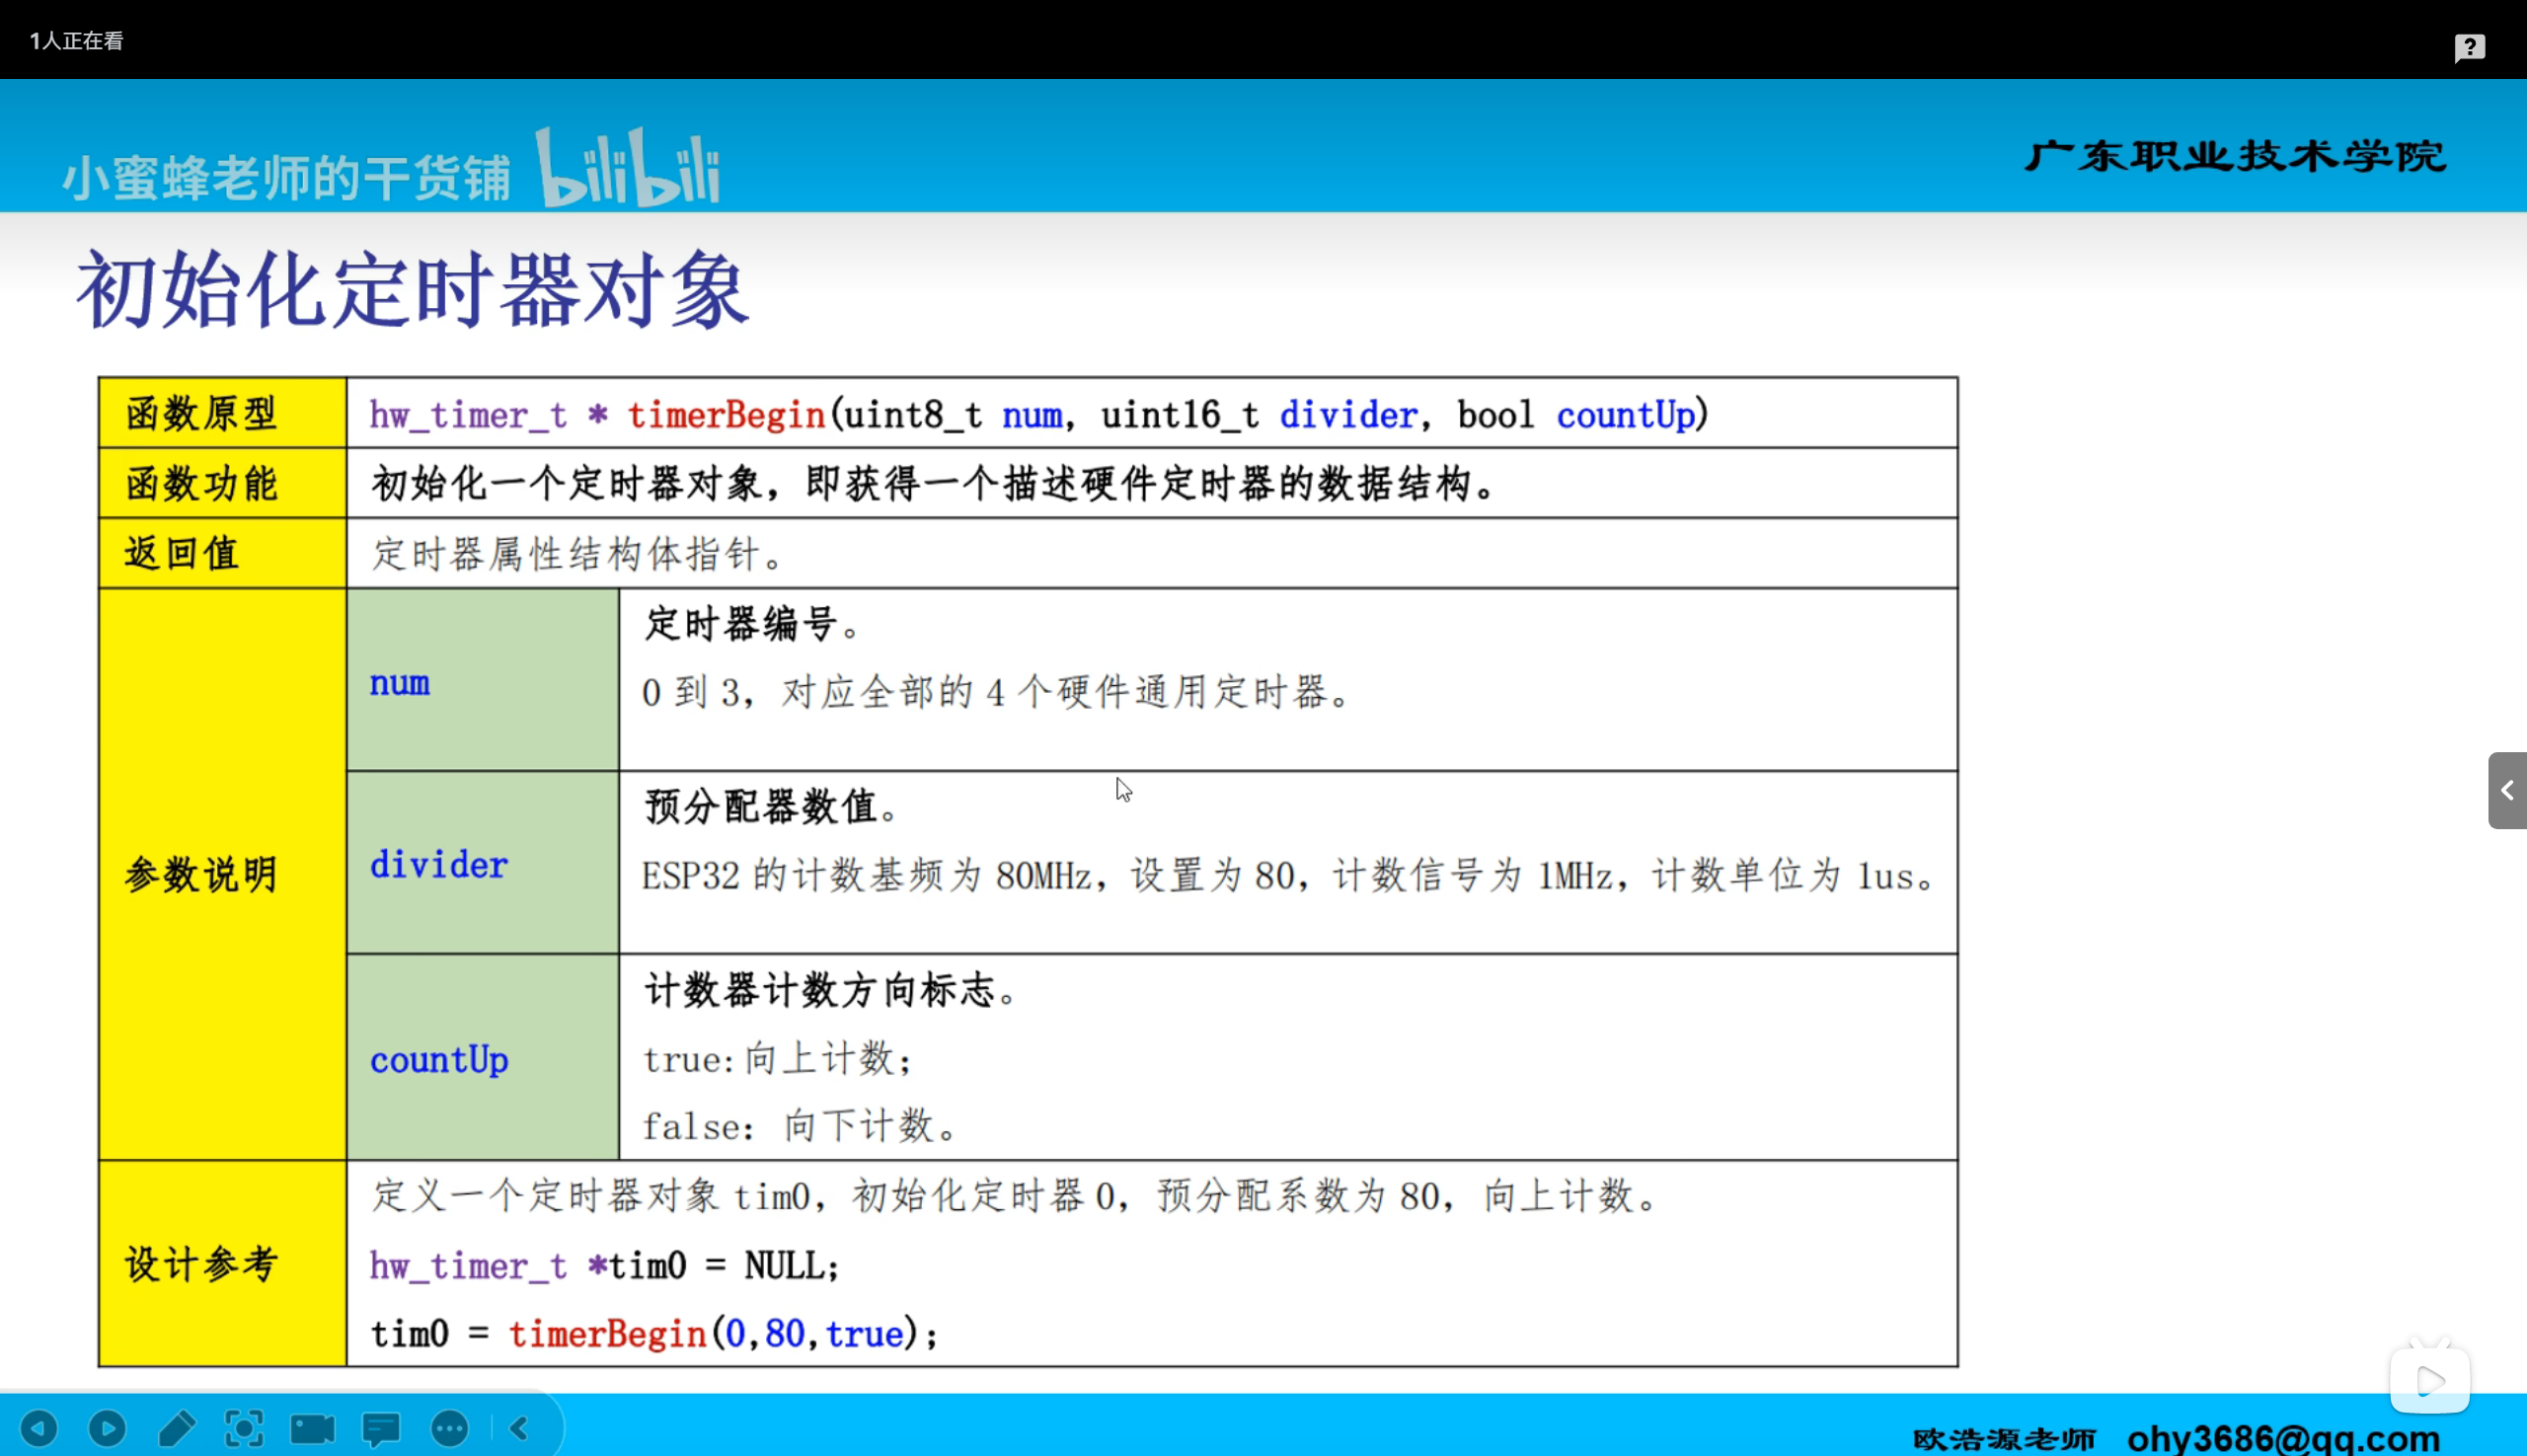
\includegraphics[width=0.6\textwidth]{Figures/TimerInit.png}
    \caption{timerBegin}
\end{figure}
函数名为: \textit{\textbf{timerBegin(参数一,参数二,参数三)} }.
\begin{itemize}
    \item 参数一:要对哪一个定时器进行操作(有定时器0,定时器一、二、三等等)
    \item 参数二:要设置的预分配系数
    \item 参数三:设置计数器计数计数方向,规定向上计数还是向下计数
    \item 返回值:返回值是一个存储着刚才配置信息的结构体指针
\end{itemize}
\newpage
\subsection{ 定时器参数配置 }
\begin{figure}[h]
    \centering
    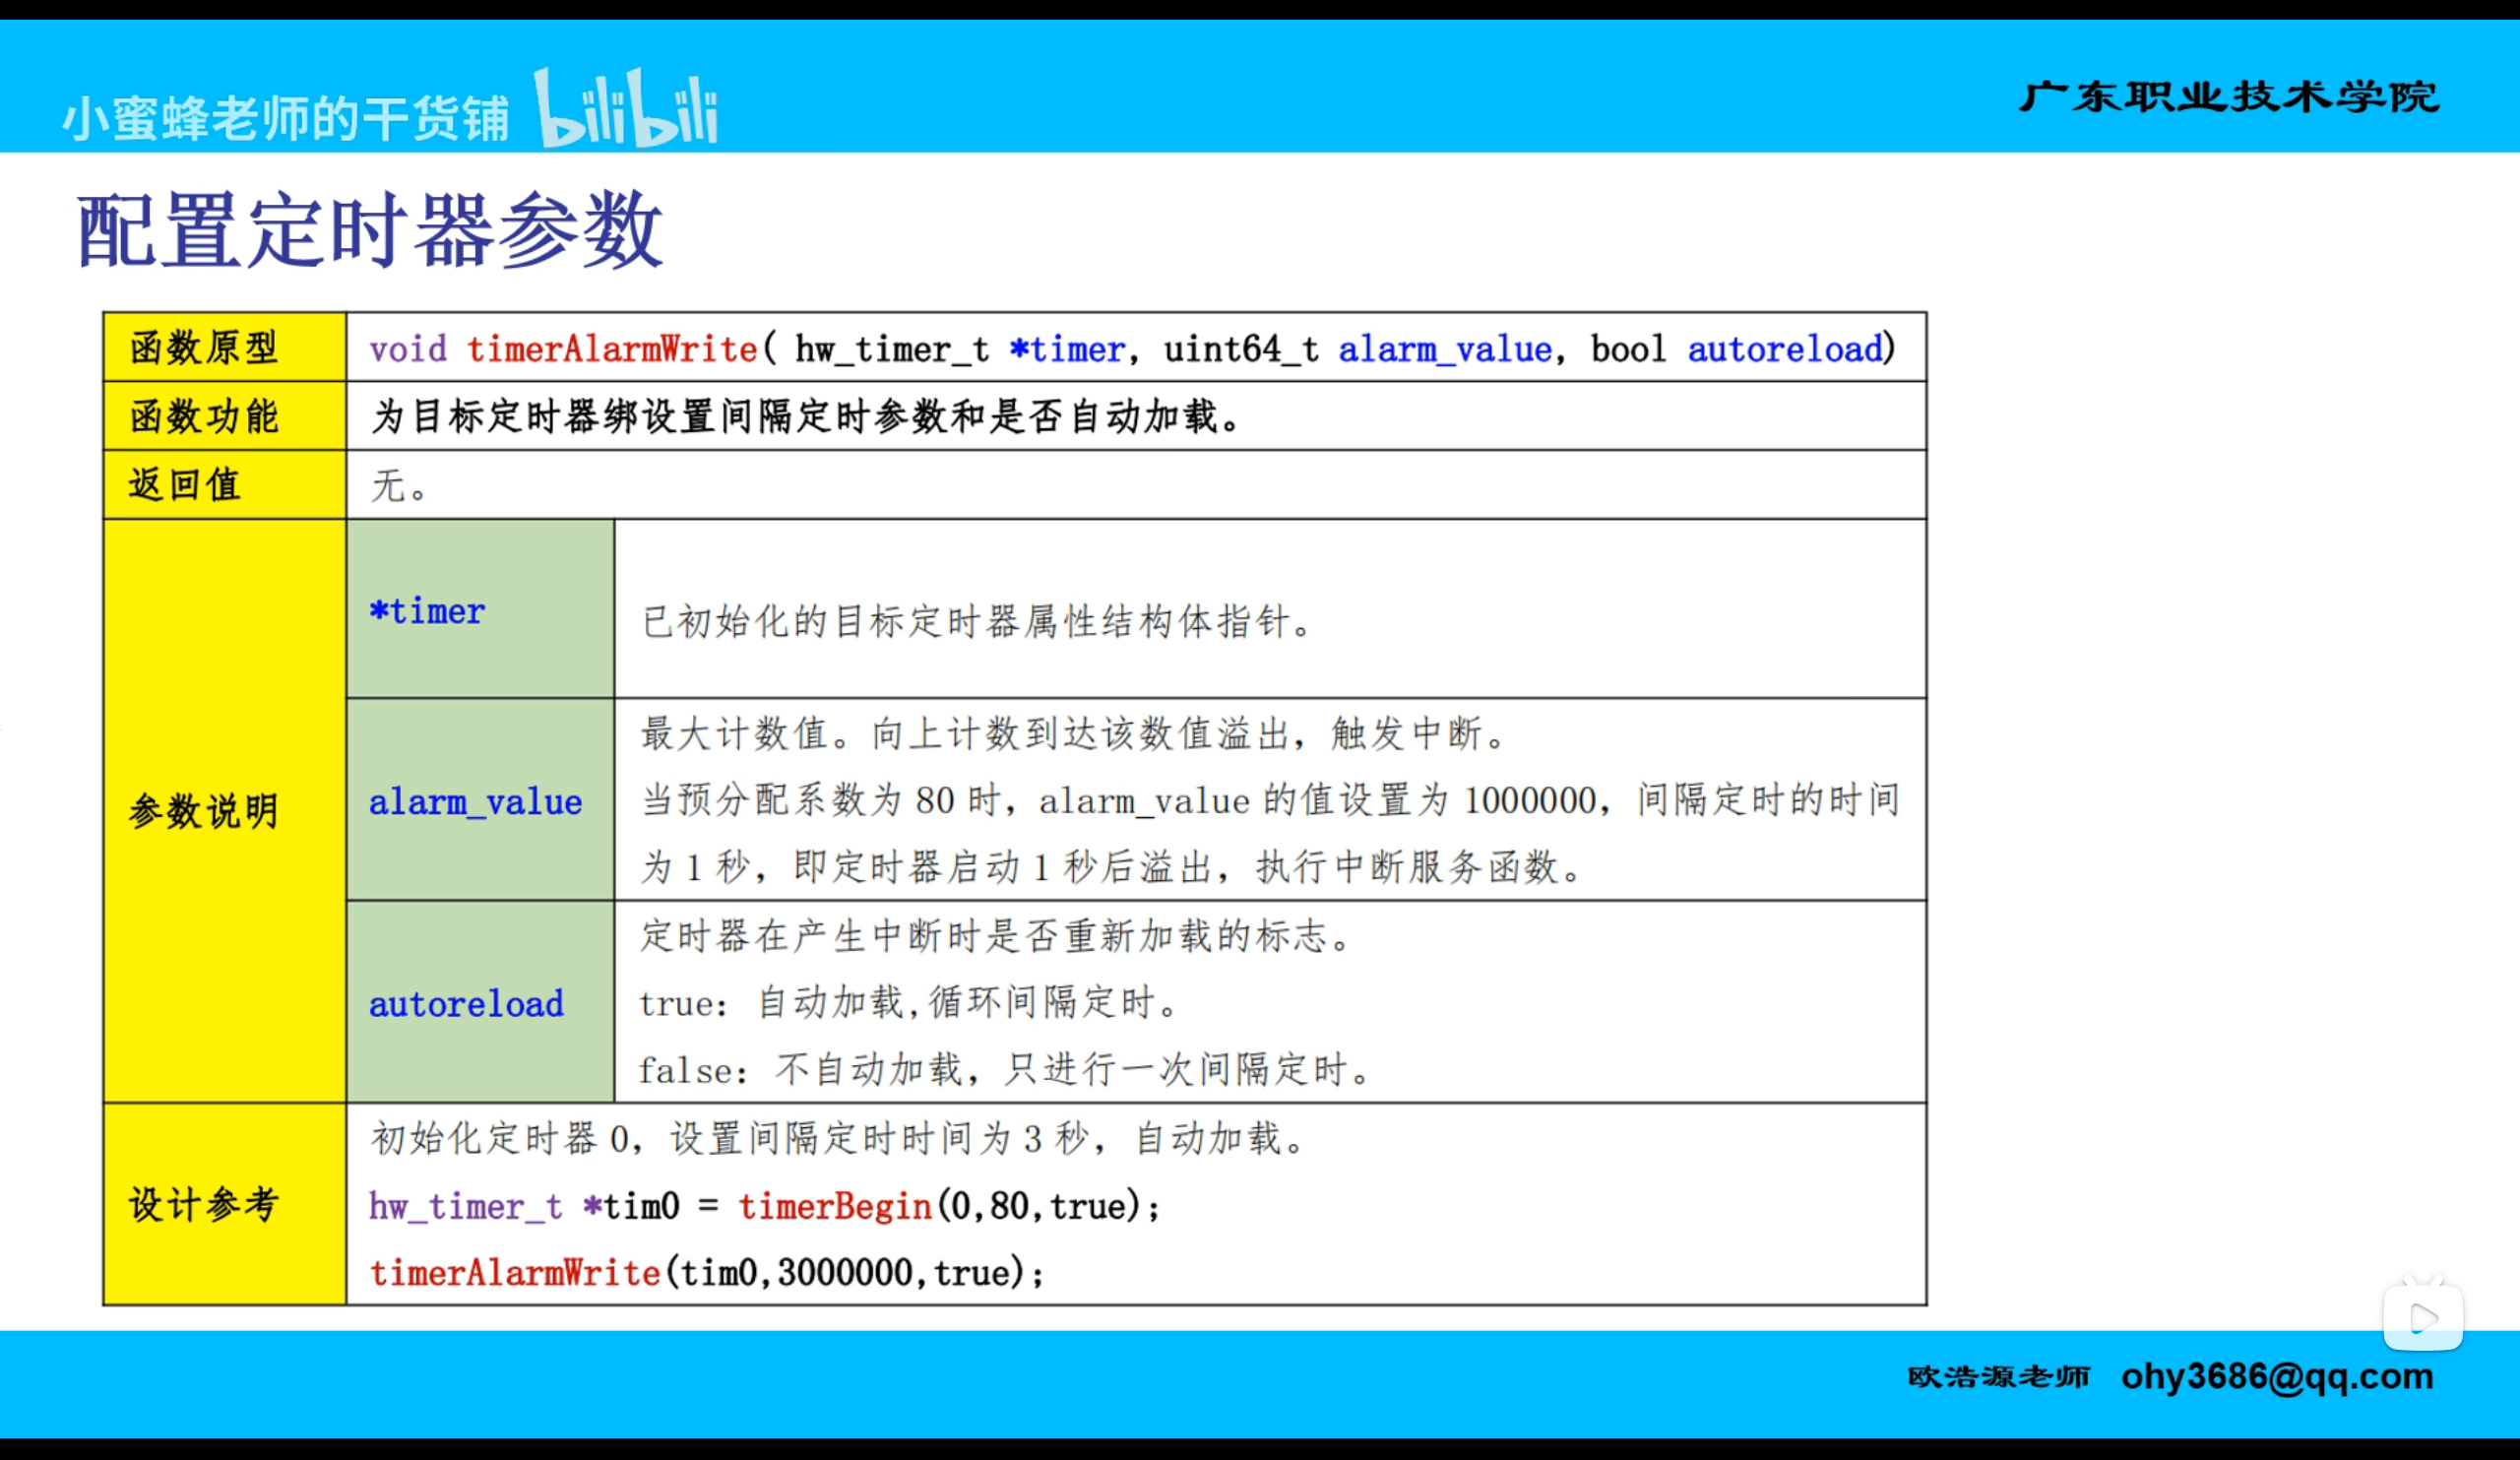
\includegraphics[width=\textwidth]{Figures/Timer_Perimiter.png}
    \caption{配置定时器参数}    
\end{figure}
函数名为: \textit{\textbf{timerAlarmWrite(参数一,参数二,参数三)}}.
\begin{itemize}
    \item 参数一:填写着要配置中断的时钟的信息的结构体指针(例如样例中给的*tim0)
    \item 参数二:最大计数值
    \item 参数三:决定是否循环调用计时器中断函数
\end{itemize}
\newpage
\subsubsection{ 定时器中断配置函数 }
\begin{figure}[h]
    \centering
    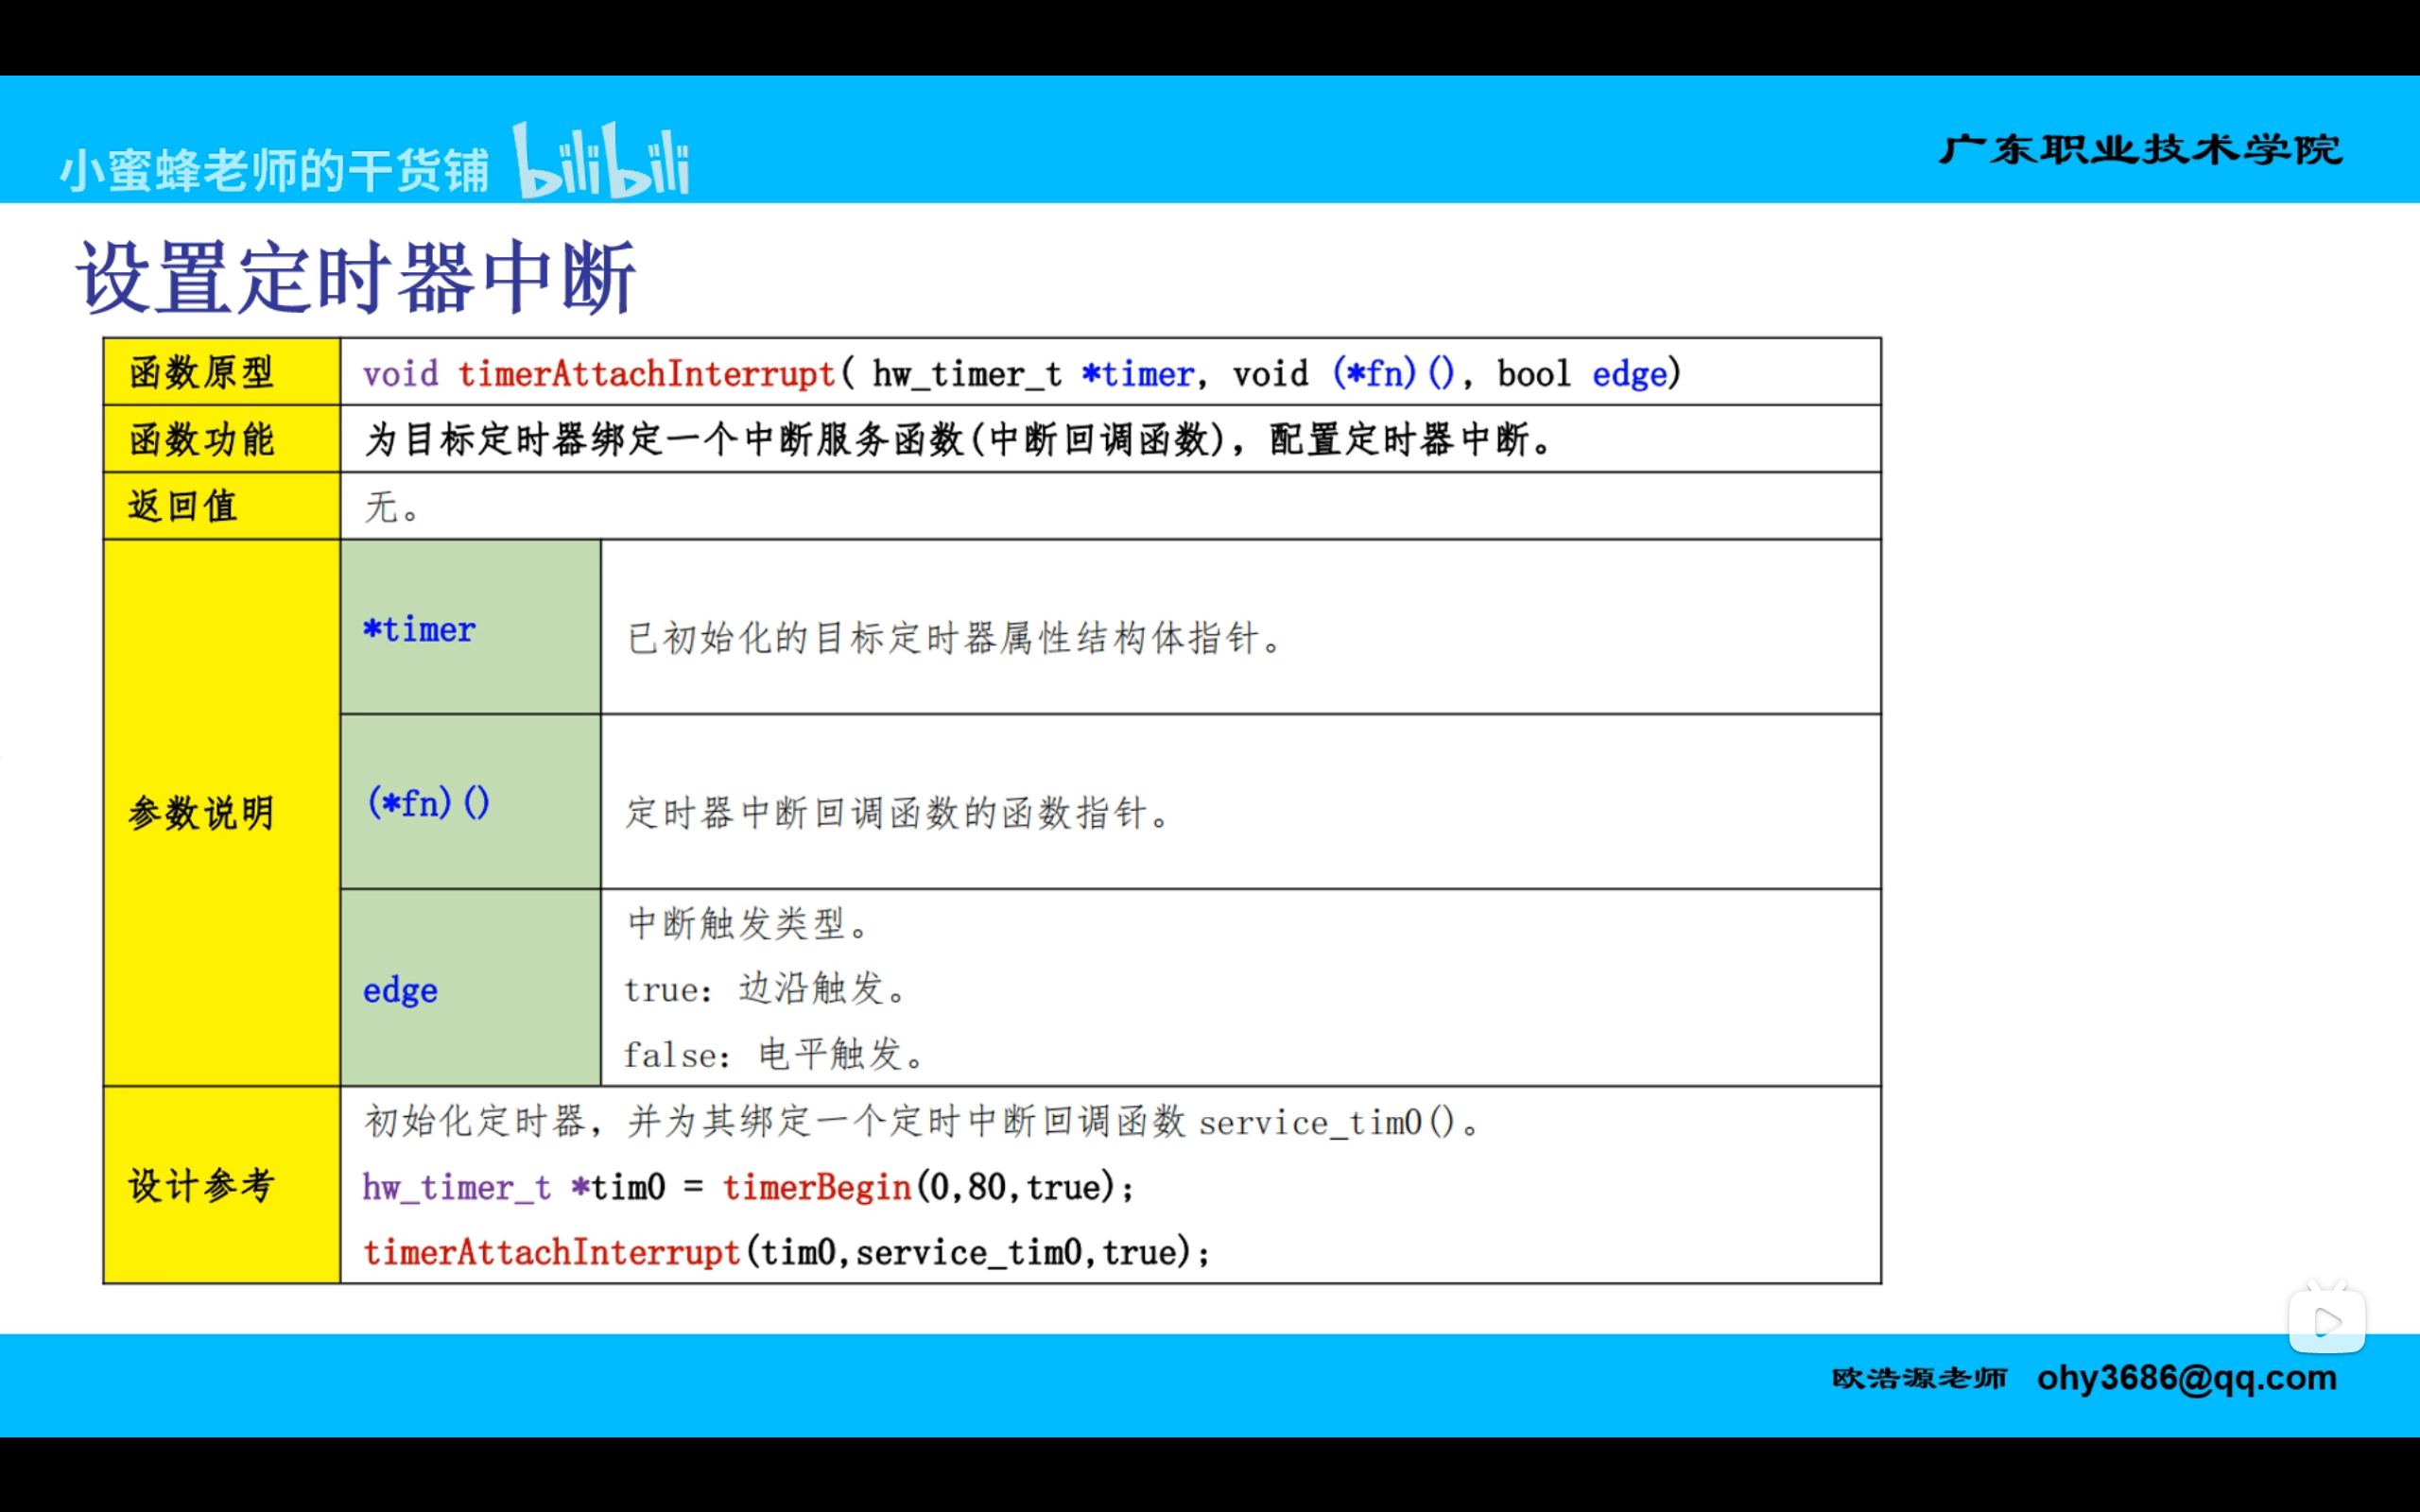
\includegraphics[width=\textwidth]{Figures/Timer_Interrupt.png}
    \caption{定时器中断配置函数}    
\end{figure}
函数名为: \textit{\textbf{void timerAttachInterrupt(参数一,参数二,参数三)}}.
\begin{itemize}
    \item 参数一:填写着要配置中断的时钟的信息的结构体指针(例如样例中给的*tim0)
    \item 参数二:发生中断时要调用的函数指针
    \item 参数三:触发中断的方式(边沿触发和电平触发)
\end{itemize}



\section{OLED的使用}
\subsection{添加驱动库文件(以SSD1306为例)}
在 PlatformIO 的 Library 中找到驱动库（以 Adafruit 的驱动库为例），点击后添加到自己的工程中。

\begin{figure}[htbp]
    \centering
    \tikzset{
        process/.style={
            rectangle, 
            minimum width=4cm, 
            minimum height=0.8cm, 
            text centered, 
            text width=4.5cm, 
            draw=black, 
            fill=blue!5,
            font=\small
        },
        arrow/.style={thick, ->, >=stealth}
    }

    \begin{tikzpicture}[node distance=1.2cm]
        \node (step1) [process] {1. 进入 PIO Home $\rightarrow$ Libraries};
        \node (step2) [process, below=of step1] {2. 搜索栏输入 ``SSD1306''};
        \node (step3) [process, below=of step2] {3. 选择 Adafruit SSD1306};
        \node (step4) [process, below=of step3] {4. 点击 ``Add to Project''};
        \node (step5) [process, below=of step4] {5. 选择当前工程并点击 Add};

        \draw [arrow] (step1) -- (step2);
        \draw [arrow] (step2) -- (step3);
        \draw [arrow] (step3) -- (step4);
        \draw [arrow] (step4) -- (step5);
    \end{tikzpicture}
    \caption{PlatformIO 添加 SSD1306 驱动库流程}
    \label{fig:pio_lib_add}
\end{figure}

添加完成后，建议检查项目根目录下的 \texttt{platformio.ini} 文件，确认 \texttt{lib\_deps} 选项中已包含 \texttt{adafruit/Adafruit SSD1306}。
\par
接下来，在代码中包含驱动库的头文件，并按照库的使用说明进行初始化和调用相关函数来控制 OLED 显示。
在不知道如何使用的时候，可以参考该库的示例代码，通常在库的安装目录下会有一个 \texttt{examples} 文件夹，里面包含了各种使用示例，可以帮助你快速上手。
亦或者你可以在添加该驱动库的界面查看一下他给的示例代码, 也可以在网上搜索一下相关的使用教程, 以便更好地理解和使用该驱动库。
\par
接下来的代码是初始化OLED显示屏的通用代码,基本不需要做什么修改, 只需要按照你使用的驱动库的要求进行相应的调整即可。
\begin{lstlisting}[language=C]
    #include <Arduino.h>

    #include <SPI.h>
    #include <Wire.h>
    #include <Adafruit_GFX.h>
    #include <Adafruit_SSD1306.h>
    #define SDA_PIN 4
    #define SCL_PIN 5

    Adafruit_SSD1306 oled = Adafruit_SSD1306(128, 64, &Wire);
    void OLED_Init(){
        Wire.begin(SDA_PIN, SCL_PIN,100000);
        oled.begin(SSD1306_SWITCHCAPVCC, 0x3c);
        oled.clearDisplay();
        oled.setTextSize(1);
        oled.setTextColor(SSD1306_WHITE);
        oled.setCursor(0, 0);
    }
\end{lstlisting}    
\subsection{ 图片数据的生成与OLED显示 }
在此次实验中,我们使用的OLED字模工具为\textbf{PCtoLCD2018},该工具可以将图片转换为适合OLED显示的字模数据。以下是使用该工具的步骤：
\begin{enumerate}
    \item 打开 PCtoLCD2018 软件。
    \item 在模式选项中选择"\textbf{图形模式}"
    \item 在设置中选择"\textbf{阴码,逐行式,顺向,C51格式,行前缀留空,行后缀只留",",确定}
    \item 点击"\textbf{打开图片}"按钮，选择需要转换的图片文件。
    \item 图片加载完成后，点击"\textbf{生成代码}"按钮，软件将自动生成适合OLED显示的字模数据，并显示在下方的文本框中。
    \item 将生成的字模数据复制到代码中，使用OLED驱动库提供的函数进行显示。
\end{enumerate}
\newpage
\begin{figure}[h]
    \centering
    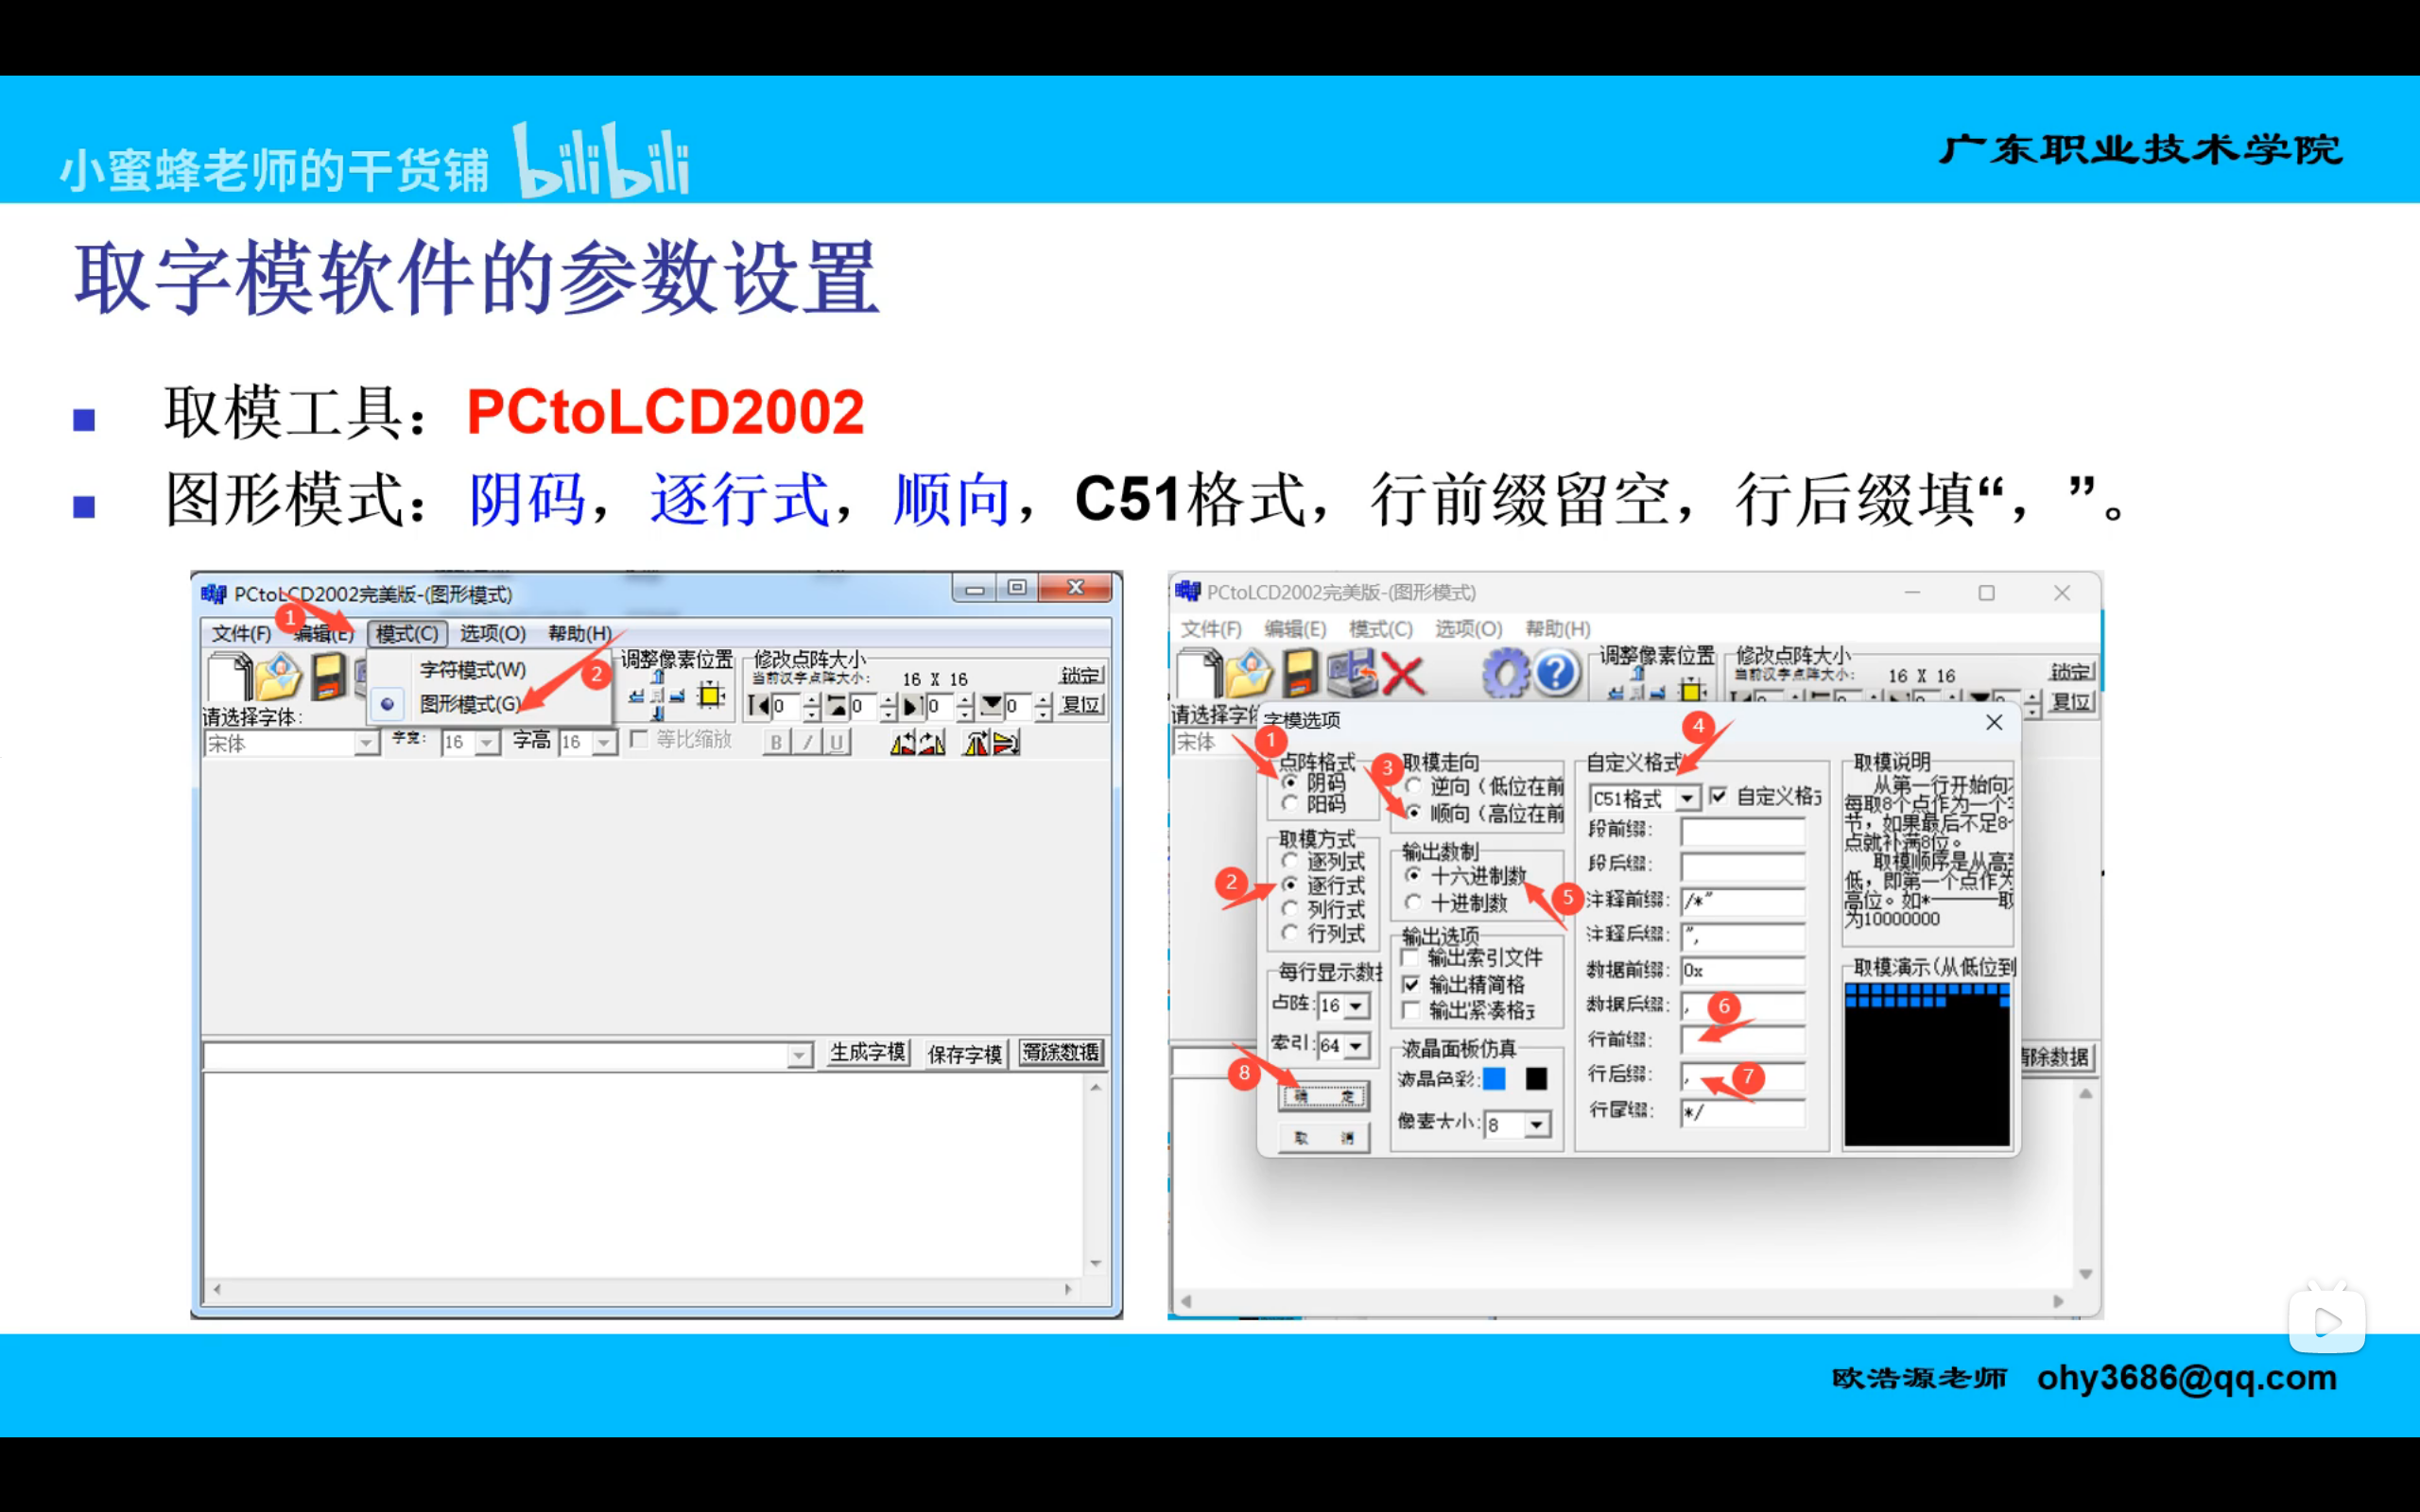
\includegraphics[width=\textwidth]{Figures/PCto.png}
    \caption{UP主的PCtoLCD2018 设置界面}
\end{figure}
需要注意的是，生成的字模数据格式必须与OLED驱动库要求的格式一致，否则可能无法正确显示图片。
对于不同的驱动库, 可能需要对生成的字模数据进行适当的调整或转换。此时可以参考该驱动库中类似drawBitmap的函数定义,
查看里面的函数实现, 以确定需要的数据格式和排列方式, 从而对生成的字模数据进行相应的修改。(如若看不懂,可以将该函数复制给AI,让它帮你分析一下需要什么样的数据格式)
\vspace{1em}

\textcolor{red}{\textbf{需要额外提醒的是}:读者对Adafruit SSD1306驱动库的drawBitmap函数进行
上述操作时会发现你最后会得出要使用阳码的结论,这是正确的。按照官方要求，本身就应该为阳码,但
不知为何UP主要使用阴码。对此作者也不是很明白，希望读者在使用过程中注意这一点。}
\newpage
\subsection{OLED显示中文汉字}
OLED显示中文汉字的步骤与显示图片类似，主要区别在于需要使用适合中文字符的字模数据。以下是具体步骤：
\begin{enumerate}
    \item 准备需要显示的中文汉字，可以是单个字符或字符串。
    \item 使用适合中文字符的字模工具（如PCtoLCD2018），设置正确的字模格式，将中文汉字转换为字模数据。UP主所设置的字模格式如下：
    \begin{figure}[h]
        \centering
        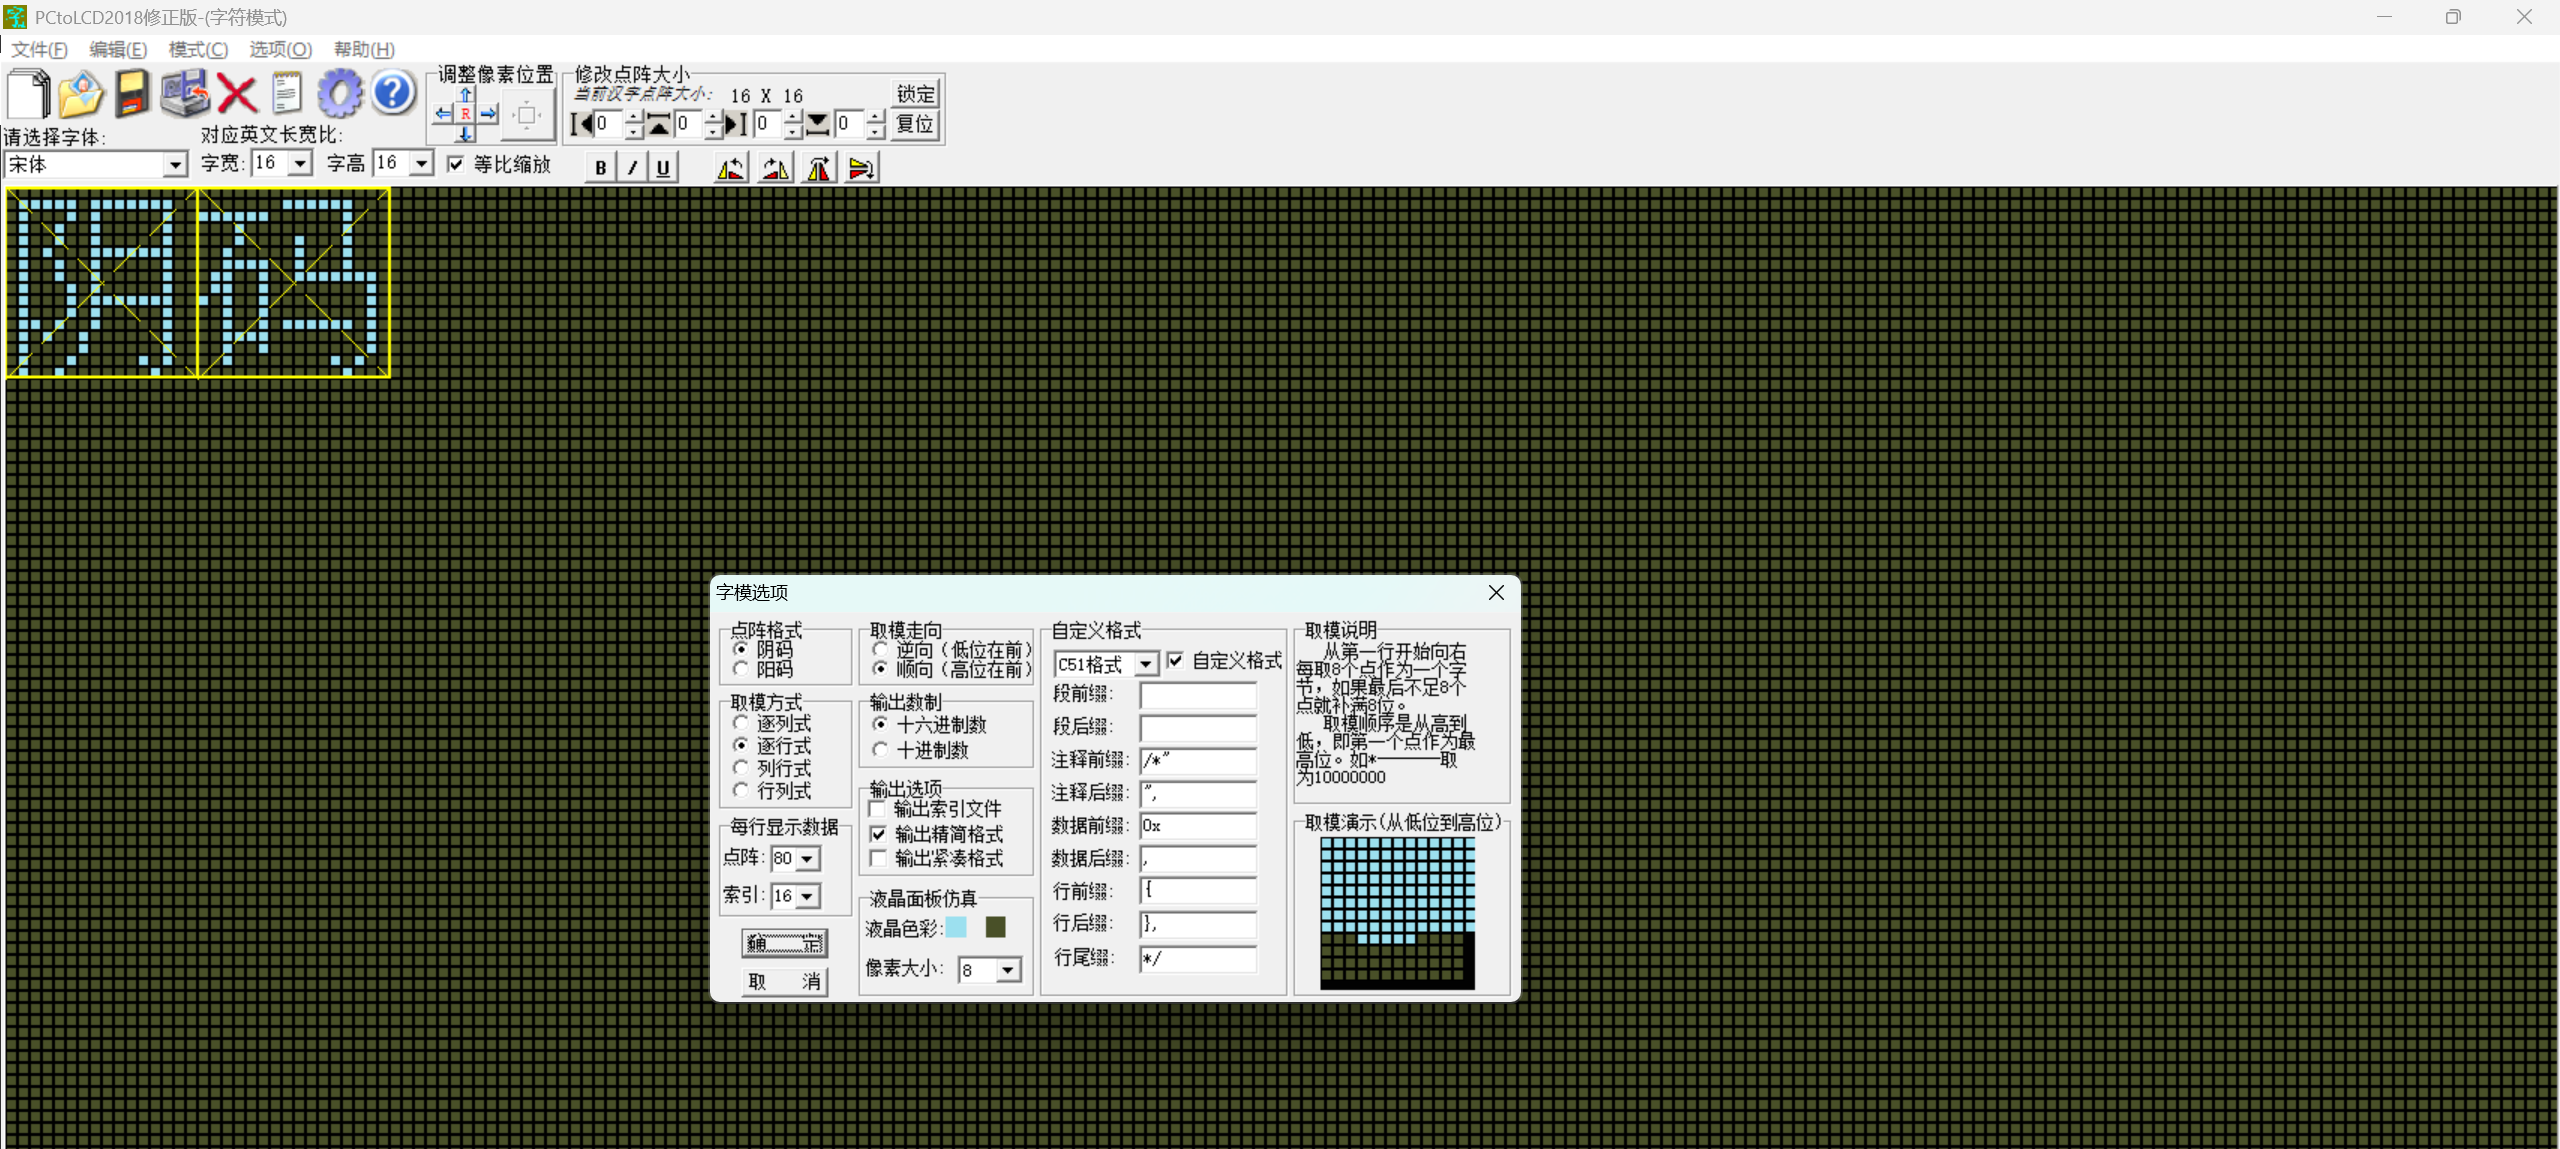
\includegraphics[width=\textwidth]{Figures/ChineseCharacters.png}
        \caption{UP主的PCtoLCD2018 设置界面-中文汉字}
    \end{figure}
    \item 将生成的字模数据复制到代码中，使用OLED驱动库提供的函数进行显示。通常，OLED驱动库会有专门的函数用于显示中文字符，确保使用正确的函数调用。
    \item 调整显示位置和字体大小，以确保中文汉字能够正确显示在OLED屏幕上。
\end{enumerate}
这是简单的汉字打印代码示例:
\begin{lstlisting}[language=C]
    void OLED_Show_Chinese(){
        oled.clearDisplay();
        /* Positive code*/
        oled.drawBitmap(0, 0, ziku[0], 16, 16, SSD1306_WHITE); 
        oled.drawBitmap(20, 0, ziku[1], 16, 16, SSD1306_WHITE);
        /* Negative code */
        oled.drawBitmap(0, 40, ziku[2], 16, 16, SSD1306_WHITE);
        oled.drawBitmap(20, 40, ziku[3], 16, 16, SSD1306_WHITE);
        oled.display();
    }
\end{lstlisting}


\end{document}